\documentclass[]{book}
\usepackage{lmodern}
\usepackage{amssymb,amsmath}
\usepackage{ifxetex,ifluatex}
\usepackage{fixltx2e} % provides \textsubscript
\ifnum 0\ifxetex 1\fi\ifluatex 1\fi=0 % if pdftex
  \usepackage[T1]{fontenc}
  \usepackage[utf8]{inputenc}
\else % if luatex or xelatex
  \ifxetex
    \usepackage{mathspec}
  \else
    \usepackage{fontspec}
  \fi
  \defaultfontfeatures{Ligatures=TeX,Scale=MatchLowercase}
\fi
% use upquote if available, for straight quotes in verbatim environments
\IfFileExists{upquote.sty}{\usepackage{upquote}}{}
% use microtype if available
\IfFileExists{microtype.sty}{%
\usepackage{microtype}
\UseMicrotypeSet[protrusion]{basicmath} % disable protrusion for tt fonts
}{}
\usepackage[margin=1in]{geometry}
\usepackage{hyperref}
\hypersetup{unicode=true,
            pdftitle={Documentation for the discoveryengine},
            pdfborder={0 0 0},
            breaklinks=true}
\urlstyle{same}  % don't use monospace font for urls
\usepackage{natbib}
\bibliographystyle{plainnat}
\usepackage{color}
\usepackage{fancyvrb}
\newcommand{\VerbBar}{|}
\newcommand{\VERB}{\Verb[commandchars=\\\{\}]}
\DefineVerbatimEnvironment{Highlighting}{Verbatim}{commandchars=\\\{\}}
% Add ',fontsize=\small' for more characters per line
\usepackage{framed}
\definecolor{shadecolor}{RGB}{248,248,248}
\newenvironment{Shaded}{\begin{snugshade}}{\end{snugshade}}
\newcommand{\AlertTok}[1]{\textcolor[rgb]{0.94,0.16,0.16}{#1}}
\newcommand{\AnnotationTok}[1]{\textcolor[rgb]{0.56,0.35,0.01}{\textbf{\textit{#1}}}}
\newcommand{\AttributeTok}[1]{\textcolor[rgb]{0.77,0.63,0.00}{#1}}
\newcommand{\BaseNTok}[1]{\textcolor[rgb]{0.00,0.00,0.81}{#1}}
\newcommand{\BuiltInTok}[1]{#1}
\newcommand{\CharTok}[1]{\textcolor[rgb]{0.31,0.60,0.02}{#1}}
\newcommand{\CommentTok}[1]{\textcolor[rgb]{0.56,0.35,0.01}{\textit{#1}}}
\newcommand{\CommentVarTok}[1]{\textcolor[rgb]{0.56,0.35,0.01}{\textbf{\textit{#1}}}}
\newcommand{\ConstantTok}[1]{\textcolor[rgb]{0.00,0.00,0.00}{#1}}
\newcommand{\ControlFlowTok}[1]{\textcolor[rgb]{0.13,0.29,0.53}{\textbf{#1}}}
\newcommand{\DataTypeTok}[1]{\textcolor[rgb]{0.13,0.29,0.53}{#1}}
\newcommand{\DecValTok}[1]{\textcolor[rgb]{0.00,0.00,0.81}{#1}}
\newcommand{\DocumentationTok}[1]{\textcolor[rgb]{0.56,0.35,0.01}{\textbf{\textit{#1}}}}
\newcommand{\ErrorTok}[1]{\textcolor[rgb]{0.64,0.00,0.00}{\textbf{#1}}}
\newcommand{\ExtensionTok}[1]{#1}
\newcommand{\FloatTok}[1]{\textcolor[rgb]{0.00,0.00,0.81}{#1}}
\newcommand{\FunctionTok}[1]{\textcolor[rgb]{0.00,0.00,0.00}{#1}}
\newcommand{\ImportTok}[1]{#1}
\newcommand{\InformationTok}[1]{\textcolor[rgb]{0.56,0.35,0.01}{\textbf{\textit{#1}}}}
\newcommand{\KeywordTok}[1]{\textcolor[rgb]{0.13,0.29,0.53}{\textbf{#1}}}
\newcommand{\NormalTok}[1]{#1}
\newcommand{\OperatorTok}[1]{\textcolor[rgb]{0.81,0.36,0.00}{\textbf{#1}}}
\newcommand{\OtherTok}[1]{\textcolor[rgb]{0.56,0.35,0.01}{#1}}
\newcommand{\PreprocessorTok}[1]{\textcolor[rgb]{0.56,0.35,0.01}{\textit{#1}}}
\newcommand{\RegionMarkerTok}[1]{#1}
\newcommand{\SpecialCharTok}[1]{\textcolor[rgb]{0.00,0.00,0.00}{#1}}
\newcommand{\SpecialStringTok}[1]{\textcolor[rgb]{0.31,0.60,0.02}{#1}}
\newcommand{\StringTok}[1]{\textcolor[rgb]{0.31,0.60,0.02}{#1}}
\newcommand{\VariableTok}[1]{\textcolor[rgb]{0.00,0.00,0.00}{#1}}
\newcommand{\VerbatimStringTok}[1]{\textcolor[rgb]{0.31,0.60,0.02}{#1}}
\newcommand{\WarningTok}[1]{\textcolor[rgb]{0.56,0.35,0.01}{\textbf{\textit{#1}}}}
\usepackage{longtable,booktabs}
\usepackage{graphicx,grffile}
\makeatletter
\def\maxwidth{\ifdim\Gin@nat@width>\linewidth\linewidth\else\Gin@nat@width\fi}
\def\maxheight{\ifdim\Gin@nat@height>\textheight\textheight\else\Gin@nat@height\fi}
\makeatother
% Scale images if necessary, so that they will not overflow the page
% margins by default, and it is still possible to overwrite the defaults
% using explicit options in \includegraphics[width, height, ...]{}
\setkeys{Gin}{width=\maxwidth,height=\maxheight,keepaspectratio}
\IfFileExists{parskip.sty}{%
\usepackage{parskip}
}{% else
\setlength{\parindent}{0pt}
\setlength{\parskip}{6pt plus 2pt minus 1pt}
}
\setlength{\emergencystretch}{3em}  % prevent overfull lines
\providecommand{\tightlist}{%
  \setlength{\itemsep}{0pt}\setlength{\parskip}{0pt}}
\setcounter{secnumdepth}{5}
% Redefines (sub)paragraphs to behave more like sections
\ifx\paragraph\undefined\else
\let\oldparagraph\paragraph
\renewcommand{\paragraph}[1]{\oldparagraph{#1}\mbox{}}
\fi
\ifx\subparagraph\undefined\else
\let\oldsubparagraph\subparagraph
\renewcommand{\subparagraph}[1]{\oldsubparagraph{#1}\mbox{}}
\fi

%%% Use protect on footnotes to avoid problems with footnotes in titles
\let\rmarkdownfootnote\footnote%
\def\footnote{\protect\rmarkdownfootnote}

%%% Change title format to be more compact
\usepackage{titling}

% Create subtitle command for use in maketitle
\newcommand{\subtitle}[1]{
  \posttitle{
    \begin{center}\large#1\end{center}
    }
}

\setlength{\droptitle}{-2em}

  \title{Documentation for the discoveryengine}
    \pretitle{\vspace{\droptitle}\centering\huge}
  \posttitle{\par}
    \author{}
    \preauthor{}\postauthor{}
    \date{}
    \predate{}\postdate{}
  
\usepackage{booktabs}

\begin{document}
\maketitle

{
\setcounter{tocdepth}{1}
\tableofcontents
}
\begin{Shaded}
\begin{Highlighting}[]
\NormalTok{knitr}\OperatorTok{::}\NormalTok{opts_chunk}\OperatorTok{$}\KeywordTok{set}\NormalTok{(}\DataTypeTok{warning =} \OtherTok{FALSE}\NormalTok{, }\DataTypeTok{message =} \OtherTok{FALSE}\NormalTok{, }\DataTypeTok{fig.path =} \StringTok{"images/"}\NormalTok{)}
\end{Highlighting}
\end{Shaded}

\hypertarget{welcome}{%
\chapter{Welcome}\label{welcome}}

\begin{figure}
\centering
\includegraphics{images/disco.gif}
\caption{\href{https://www.youtube.com/watch?v=uxi73RQlLB8}{Did I mention that I like to dance?}}
\end{figure}

Welcome to the introduction to and extended documentation for the discoveryengine! The discoveryengine, also known as ``Disco Engine'' or just ``Disco,'' is a tool enabling Prospect Development staff to do custom prospecting, written in the R programming language. For more information, see \protect\hyperlink{what-is-disco}{What is the Disco Engine?}

If you are already familiar with the Disco Engine, and looking for some quick tips to refresh your memory, check out the \protect\hyperlink{cheat-sheet}{cheat sheet}.

Though the Disco Engine is written in R, you don't need to have any experience using R in order to get started. That said, if you're brand new to R and RStudio, check out our brief \protect\hyperlink{r-intro}{introduction to R and RStudio}.

Otherwise, feel free to read this document in order, or to jump around or just bookmark it and refer to it as needed. You may find the search feature helpful, you can access it by clicking on the little magnifying glass at the top of the screen.

\hypertarget{contribute-to-the-disco-engine}{%
\section{Contribute to the Disco Engine}\label{contribute-to-the-disco-engine}}

The Disco Engine is a tool made by and for Prospect Development. If you see something that doesn't work correctly, or documentation that could be made clearer, or a widget that would be useful that isn't implemented, or anything at all that could be improved in the Disco Engine, please submit an issue by clicking on the green ``New Issue'' button on the \href{https://github.com/tarakc02/discoveryengine/issues}{Disco engine issues page}.

\hypertarget{contribute-to-this-documentation}{%
\section{Contribute to this documentation}\label{contribute-to-this-documentation}}

This site is a work in progress. One way you can help is to report any mistakes you find (typos, spelling mistakes, grammatical errors) or any areas that could be explained better (if something was not clear to you, there's a good chance it won't be clear to others either). This documentation site has its own \href{https://github.com/tarakc02/discodocs/issues}{Disco-docs issues page} -- click on the green ``New Issue'' button and enter a short message explaining what's wrong. If you'd like to suggest edits directly, you can do so by clicking on the pen-and-paper icon at the top of any page on this site (guide coming soon). Thank you!

\hypertarget{part-preliminaries}{%
\part{Preliminaries}\label{part-preliminaries}}

\hypertarget{what-is-disco}{%
\chapter{What is the Disco Engine?}\label{what-is-disco}}

If you happen to have an APRA account, this \href{http://connections.aprahome.org/blog/building-the-discovery-engine}{article in APRA Connections magazine} is a good introduction. If you don't have an APRA account, then read on . . .

The Discovery Engine, or Disco Engine, is a prospecting tool that empowers Prospect Development staff to precisely define (and pull together) constitutencies for their fundraising clients. It does so by providing two complementary resources: a \emph{vocabulary and grammar} for specifying constituencies, and tools to facilitate \emph{discovery} of constituencies.

\hypertarget{vocabulary-and-grammar}{%
\section{Vocabulary and Grammar}\label{vocabulary-and-grammar}}

The Disco Engine is based on the idea that a constituency can be defined using one or more \emph{predicates} (such as ``majored in math'' or ``attended a Discover Cal event''), where multiple predicates are combined using ``and'', ``or'', or ``but not.'' To illustrate, here is a sample constituency definition for the department of mathematics:

\begin{quote}
\emph{majored in mathematics} \textbf{or} \emph{has given to the math department}
\end{quote}

The constituency is then just any individual who fits the definition.

The most basic tool that the Disco Engine provides is called a \protect\hyperlink{working-with-widgets}{widget}, which is a tool for generating a simple predicate. For instance, the widget \texttt{majored\_in} allows us to build the first part of our example definition:

\begin{Shaded}
\begin{Highlighting}[]
\KeywordTok{majored_in}\NormalTok{(mathematics)}
\end{Highlighting}
\end{Shaded}

Furthermore, the Disco Engine provides the following connectors to \emph{combine} predicates in order to create more complex definitions:

\begin{itemize}
\tightlist
\item
  \texttt{\%and\%}
\item
  \texttt{\%or\%}
\item
  \texttt{\%but\_not\%}
\end{itemize}

So in the language of the Disco Engine, our definition would look like:

\begin{Shaded}
\begin{Highlighting}[]
\KeywordTok{majored_in}\NormalTok{(mathematics) }\OperatorTok\StringTok{ }\KeywordTok{gave_to_department}\NormalTok{(mathematics)}
\end{Highlighting}
\end{Shaded}

There is no limit to the number of predicates that can be strung together to form a definition:

\begin{Shaded}
\begin{Highlighting}[]
\KeywordTok{majored_in}\NormalTok{(mathematics) }\OperatorTok
\StringTok{    }\KeywordTok{gave_to_department}\NormalTok{(mathematics) }\OperatorTok
\StringTok{    }\KeywordTok{lives_in_msa}\NormalTok{(san_francisco)}
\end{Highlighting}
\end{Shaded}

These definitions can quickly become very complex. To manage that complexity, the Disco Engine provides the ability to \emph{assign} names to definitions, that can then be used to construct more complex definitions:

\begin{Shaded}
\begin{Highlighting}[]
\NormalTok{is_math_constituent =}\StringTok{ }\KeywordTok{majored_in}\NormalTok{(mathematics) }\OperatorTok\StringTok{ }
\StringTok{    }\KeywordTok{gave_to_department}\NormalTok{(mathematics)}

\NormalTok{local_math_constituent =}\StringTok{ }\NormalTok{is_math_constituent }\OperatorTok
\StringTok{    }\KeywordTok{lives_in_msa}\NormalTok{(san_francisco)}

\NormalTok{parent_of_local_math_constituent =}\StringTok{ }\KeywordTok{parent_of}\NormalTok{(local_math_constituent)}
\end{Highlighting}
\end{Shaded}

Together, the collection of predicates, the logical operators, and the ability to assign names form an expressive language for describing custom constituencies for a variety of purposes. Best of all, the Disco Engine gives us the ability to pull the IDs of a defined constituency from the database!

\begin{Shaded}
\begin{Highlighting}[]
\KeywordTok{display}\NormalTok{(parent_of_local_math_constituent)}
\end{Highlighting}
\end{Shaded}

\begin{verbatim}
## # A tibble: 561 x 1
##    entity_id
##        <dbl>
##  1      1168
##  2      4522
##  3      6322
##  4      6326
##  5      7644
##  6     11512
##  7     23989
##  8     24151
##  9     24247
## 10     26492
## # … with 551 more rows
\end{verbatim}

\hypertarget{facilitating-discovery}{%
\section{Facilitating discovery}\label{facilitating-discovery}}

Having a clear language for prospecting and defining constituencies is nice, but Prospect Development is increasingly being asked to do affinity-based prospecting, which often involves defining new constituencies that don't have clear-cut coding associated with them yet, or digging into student activity, interest, affiliation, and other codes to figure out which ones might fit the constituency to be defined. That need motivates the Disco Engine's bots, such as the \protect\hyperlink{brainstorm-bot}{brainstorm bot} and the \protect\hyperlink{matrix-bot}{matrix bot}. We've already seen examples of using predicates to find individuals, but bots allow us to search for predicates.

\begin{Shaded}
\begin{Highlighting}[]
\KeywordTok{brainstorm_bot}\NormalTok{(}\StringTok{"robot*"}\NormalTok{, }\StringTok{"artificial intelligence"}\NormalTok{, }\StringTok{"AI"}\NormalTok{)}
\end{Highlighting}
\end{Shaded}

\begin{verbatim}
## attended_event 
##     8760: Robots on the Edge:Intelligent Machines
##     9139: AI Energy Alumni Panel & Firm Night
##     8759: Fireside Chat w/Tom Siebel:  AI and IoT
##     9141: AI Business Behaving Well: Social Resp.
##     9361: Inclusive AI: Technology and Policy
##     9140: AI Career Coach Information Session
##     6724: Haas East Bay Chp Robotic Event 06-18-14
##     9325: BARS 2017: Bay Area Robotics Symposium
##     9136: AI Getting Smart about Start-Ups
##     9497: Putting AI to Work: Tech & Policy
##     9498: WIT: Future of AI
##     8761: Silicon Valley Forum: Medical Robotics
##     9147: AI Coaching with Niandong Wang MBA '04
##     9280: AL SD Content AI Impact on Life
##     9431: SVF: Robots on the Edge
##     9138: AI Learn how to Write a Powerful Resume
## attended_hs 
##     471828: Cb-Ai Operations S&L
## fec_gave_to_committee 
##     C00596908: ROBOTECHNOLOGY INC C.R.
##     C00521765: LIQUID ROBOTICS INC POLITICAL ACTION COMMITTEE (LIQUID ROBOTICS PAC)
##     C00144261: APPRAISAL INSTITUTE PAC (AI PAC)
##     C00717249: RALLY ROBOT ZAPS AOC
##     C00582767: CAMPAIGN FOR A FEDERAL ROBOTICS COMMISSION
##     C00635748: AI PAC
##     C00717074: RALLY ROBOT 2020
## has_interest 
##     AIN: Artificial Intelligence
##     ROB: Robotics
## participated_in 
##     UROB: Robotmedia Presents
##     RENY: Robotics & Engineering for Youth
##     ENRO: Cal Robotics
## sec_filed 
##     1409269: Restoration Robotics, Inc.
##     1528557: Corindus Vascular Robotics, Inc.
##     1409269: Restoration Robotics Inc
\end{verbatim}

\hypertarget{r-intro}{%
\chapter{Introduction to R and RStudio}\label{r-intro}}

The discoveryengine works best when used with RStudio. Watch this video for a quick tour around RStudio:

\hypertarget{installation}{%
\chapter{Installation}\label{installation}}

Discoveryengine (and all packages we use in Prospect Developmemt) is installed on the R drive. The most important step to make sure you can access these packages is to set up your default library path to the shared packages repository.

Run a quick test to see your current library path:

\begin{Shaded}
\begin{Highlighting}[]
\KeywordTok{.libPaths}\NormalTok{()}
\end{Highlighting}
\end{Shaded}

The first result returned shoud be ``R:/Prospect Development/Prospect Analysis/pd-shared-r-packages''. If it's not, follow the steps below to change your default library path.

Step 1: Open a new RStudio session and run the following script:

\begin{Shaded}
\begin{Highlighting}[]
\CommentTok{# the first part sets up the new package directory}
\NormalTok{package_dir <-}\StringTok{ "R:/Prospect Development/Prospect Analysis/pd-shared-r-packages"}
\ControlFlowTok{if}\NormalTok{ (}\OperatorTok{!}\KeywordTok{dir.exists}\NormalTok{(package_dir)) }\KeywordTok{dir.create}\NormalTok{(package_dir, }\DataTypeTok{recursive =} \OtherTok{TRUE}\NormalTok{)}

\CommentTok{# then make a configuration file that notifies R of the new package directory}
\CommentTok{# change [username] to your actual username in your P drive - usually LastNameFirstInitial}
\NormalTok{env_file <-}\StringTok{ "P:/[username]/.Renviron"}
\ControlFlowTok{if}\NormalTok{ (}\OperatorTok{!}\KeywordTok{file.exists}\NormalTok{(env_file)) }\KeywordTok{file.create}\NormalTok{(env_file)}

\CommentTok{# and add the new location to the configuration file}
\KeywordTok{cat}\NormalTok{(}\StringTok{"}\CharTok{\textbackslash{}n}\StringTok{R_LIBS_USER='"}\NormalTok{, package_dir, }\StringTok{"'"}\NormalTok{, }
    \DataTypeTok{sep =} \StringTok{""}\NormalTok{, }\DataTypeTok{file =}\NormalTok{ env_file, }\DataTypeTok{append =} \OtherTok{TRUE}\NormalTok{)}
\end{Highlighting}
\end{Shaded}

Step 2:

Find the newly created .Renviron file. It will be in your P drive.

Step 3:

Move the .Renviron file to your Documents folder. This should be located in D:\textbackslash Users\textbackslash{[}username{]}\textbackslash Documents. Simply drag and drop.

Step 4:

Quit your current RStudio session and open a new one. Try running the following test again:

\begin{Shaded}
\begin{Highlighting}[]
\KeywordTok{.libPaths}\NormalTok{()}
\end{Highlighting}
\end{Shaded}

If the PD shared packages depository is returned, you are ready to start using Disco Engine. If not, contact the Analytics Team to troubleshoot your situation.

\hypertarget{before-you-continue}{%
\section{Before you continue}\label{before-you-continue}}

At this point, you should have already:
- tested your CDW connection
- installed \texttt{getcdw}
- run a test query

If you haven't completed all of those items, head over to section \protect\hyperlink{test-cdw}{Test CDW} and complete those steps, and then return here.

\hypertarget{a-disco-test}{%
\section{A disco test}\label{a-disco-test}}

In order to make sure everything is working properly, we'll run a quick disco test:

\begin{Shaded}
\begin{Highlighting}[]
\CommentTok{# you'll always load the discoveryengine package before doing anythying else}
\KeywordTok{library}\NormalTok{(discoveryengine)}
\CommentTok{# make sure we can create a disco definition}
\NormalTok{high_cap =}\StringTok{ }\KeywordTok{has_capacity}\NormalTok{(}\DecValTok{1}\NormalTok{)}
\CommentTok{# make sure that things print properly}
\NormalTok{high_cap}
\end{Highlighting}
\end{Shaded}

\begin{verbatim}
## LISTBUILDER DEFINITION (type: entity_id)
## .   source: d_entity_mv.entity_id (entity_id)
## .   logic: capacity_rating_code IN (1)
\end{verbatim}

\begin{Shaded}
\begin{Highlighting}[]
\CommentTok{# make sure we can send the defintion to the data warehouse}
\KeywordTok{display}\NormalTok{(high_cap)}
\end{Highlighting}
\end{Shaded}

\begin{verbatim}
## # A tibble: 298 x 1
##    entity_id
##        <dbl>
##  1      1969
##  2      3105
##  3      3422
##  4      7011
##  5      7644
##  6     12178
##  7     12453
##  8     17464
##  9     18139
## 10     20125
## # … with 288 more rows
\end{verbatim}

If you got this far without any problems, then congrats! You are a disco dancer!

\hypertarget{part-basics}{%
\part{Basics}\label{part-basics}}

\hypertarget{intro-example}{%
\chapter{An introductory example}\label{intro-example}}

Before diving in to details, let's work through a simple real-life example. We'll explain the functions used in more detail in later sections, but here you can see what the tool looks like in action.

Here is our scenario: A fundraiser just called, and is trying to organize an event in San Francisco that will feature a well-known technologist. She wants you to help her find prospects to invite to the event. We start out by loading the discoveryengine:

\begin{Shaded}
\begin{Highlighting}[]
\KeywordTok{library}\NormalTok{(discoveryengine)}
\end{Highlighting}
\end{Shaded}

\hypertarget{develop-a-strategy}{%
\section{Develop a strategy}\label{develop-a-strategy}}

You might already be thinking of what sorts of prospects we should look for. That's good! There are countless ways to respond to this request, and you'll have to rely on your own expertise in order to know who to include on a potential invite list. For this example, I'll use the following definition of a good prospect:

\begin{itemize}
\tightlist
\item
  has demonstrated an interest in technology, and \ldots{}
\item
  lives or works in/near San Francisco
\end{itemize}

Note that we now have a pretty clear idea of who to look for, but we need more precision. For instance, what constitutes a ``demonstrated interest in technology?'' What does it mean to be ``in/near San Francisco?'' In day-to-day conversations, we don't necessarily need that level of precision to understand one another, but since we'll need to translate this request into language a computer can understand, the more precision the better. I'll define a ``demonstrated interest in technology'' as having either an interest code or a philanthropic affinity related to technology, and ``in/near San Francisco'' as anywhere that falls into the San Francisco Metropolitan Statistical Area (MSA).

\hypertarget{intro-example-create-def}{%
\section{Create the definition}\label{intro-example-create-def}}

So now that we have a precise idea of who we want to find, we can create a definition that the computer will understand. This is important, since our computer is the only link we have to the CADS Data Warehouse. We can give it a precise definition in a language that it understands, and it will then relay our request to the CADS Data Warehouse. The CADS data warehouse can then search for people who meet our definition, and send them back to the computer, which will then display the list to us.

Ideally, our definition would look like this: \texttt{has\_tech\_interest\ \%and\%\ is\_in\_sf}. Of course, we haven't defined those pieces yet, so just typing that in will result in an error

\begin{Shaded}
\begin{Highlighting}[]
\NormalTok{has_tech_interest }\OperatorTok\StringTok{ }\NormalTok{is_in_sf}
\end{Highlighting}
\end{Shaded}

\begin{verbatim}
## Error in operate(block1, block2, "intersect"): object 'has_tech_interest' not found
\end{verbatim}

But still we've made progress. We broke a big problem (``define a prospect for this SF tech event'') into two smaller problems (``define having a tech interest'' and ``define being in San Francisco''). Let's tackle each of these one by one. We start by defining \texttt{has\_tech\_interest}. Recall that we decided to use interest codes and philanthropic affinities here. I happen to already know that there is an interest code for ``technology'', but I'm less familiar with the philanthropic affinities area. So I'll use the search feature that is built into most widgets, accessed by entering a question mark followed by a search term into the widget:

\begin{Shaded}
\begin{Highlighting}[]
\KeywordTok{has_philanthropic_affinity}\NormalTok{(?tech)}
\end{Highlighting}
\end{Shaded}

\begin{verbatim}
## Regular codes and synonyms:
##             synonym code
##  science_technology   ST
\end{verbatim}

Ah, ok. I can use either the code \texttt{ST} or the synonym \texttt{science\_technology}.

\begin{Shaded}
\begin{Highlighting}[]
\NormalTok{has_tech_interest =}\StringTok{ }\KeywordTok{has_interest}\NormalTok{(technology) }\OperatorTok
\StringTok{    }\KeywordTok{has_philanthropic_affinity}\NormalTok{(science_technology)}
\end{Highlighting}
\end{Shaded}

We use \texttt{\%or\%} as the connector here because we're interested in anyone who has either one of these characteristics. We now move to defining \texttt{is\_in\_sf}. We'd like to look for anyone who lives or works in San Francisco:

\begin{Shaded}
\begin{Highlighting}[]
\NormalTok{is_in_sf =}\StringTok{ }\KeywordTok{lives_in_msa}\NormalTok{(san_francisco) }\OperatorTok
\StringTok{    }\KeywordTok{works_in_msa}\NormalTok{(san_francisco)}
\end{Highlighting}
\end{Shaded}

We are now able to create our full definition by combining the pieces:

\begin{Shaded}
\begin{Highlighting}[]
\NormalTok{event_prospect =}\StringTok{ }\NormalTok{has_tech_interest }\OperatorTok\StringTok{ }\NormalTok{is_in_sf}
\end{Highlighting}
\end{Shaded}

\hypertarget{send-the-definition-to-the-cdw}{%
\section{Send the definition to the CDW}\label{send-the-definition-to-the-cdw}}

As we discussed in the previous section, now that we have an official definition we can send it to the data warehouse, and see if the data warehouse finds anyone who fits. You can see the definition for yourself by just typing the name of it, though it is now written in a language for the computer to understand and may look intimidating to us humans:

\begin{Shaded}
\begin{Highlighting}[]
\NormalTok{event_prospect}
\end{Highlighting}
\end{Shaded}

\begin{verbatim}
## LISTBUILDER DEFINITION (type: entity_id)
## .   operator (LS69): intersect
## .   left (LS69): 
## .   .   operator (LE58): union all
## .   .   left (LE58): 
## .   .   .   source: d_bio_interest_mv.entity_id (entity_id)
## .   .   .   logic: 
## .   .   .   .   interest_code IN ('TEC')
## .   .   .   .   stop_dt is null
## .   .   right (LE58): 
## .   .   .   source: d_oth_phil_affinity_mv.entity_id (entity_id)
## .   .   .   logic: 
## .   .   .   .   other_affinity_type IN ('ST')
## .   .   .   .   sum(gift_amt) >= 0.0
## .   right (LS69): 
## .   .   operator (HZ38): union all
## .   .   left (HZ38): 
## .   .   .   source: d_bio_address_mv.entity_id (entity_id)
## .   .   .   logic: 
## .   .   .   .   geo_metro_area_code IN ('41860')
## .   .   .   .   addr_type_code IN ('H')
## .   .   .   .   contact_type_desc IN ('ADDRESS')
## .   .   .   .   addr_status_code IN ('A', 'K')
## .   .   right (HZ38): 
## .   .   .   source: d_bio_address_mv.entity_id (entity_id)
## .   .   .   logic: 
## .   .   .   .   geo_metro_area_code IN ('41860')
## .   .   .   .   addr_type_code IN ('B', 'I')
## .   .   .   .   contact_type_desc IN ('ADDRESS')
## .   .   .   .   addr_status_code IN ('A', 'K')
\end{verbatim}

In order to send the definition to the data warehouse, retrieve the results, and show them to us, we use the \texttt{display} function:

\begin{Shaded}
\begin{Highlighting}[]
\KeywordTok{display}\NormalTok{(event_prospect)}
\end{Highlighting}
\end{Shaded}

\begin{verbatim}
## # A tibble: 1,104 x 1
##    entity_id
##        <dbl>
##  1       529
##  2       616
##  3      3422
##  4      5280
##  5      5573
##  6      5833
##  7      6622
##  8      6886
##  9      7995
## 10      9783
## # … with 1,094 more rows
\end{verbatim}

Of course, we are probably interested in exporting this savedlist to a file, so that we might load it into CADS and run CADSmart reports on it. Conveniently, we can just do that by adding a filename:

\begin{Shaded}
\begin{Highlighting}[]
\KeywordTok{display}\NormalTok{(event_prospect, }\DataTypeTok{file =} \StringTok{"sf-tech-prospects"}\NormalTok{)}
\end{Highlighting}
\end{Shaded}

Now when I look over at my working directory, there's a new file called \texttt{sf-tech-prospects.csv}

\hypertarget{working-with-widgets}{%
\chapter{Working with widgets}\label{working-with-widgets}}

So far, we've used widgets in some simple examples. In this section, we'll explore widgets in some more detail. As always, we'll begin by loading the \texttt{discoveryengine}:

\begin{Shaded}
\begin{Highlighting}[]
\KeywordTok{library}\NormalTok{(discoveryengine)}
\end{Highlighting}
\end{Shaded}

\hypertarget{working-with-finding-widgets}{%
\section{Finding widgets}\label{working-with-finding-widgets}}

There are two main ways to find widgets. The first is to use the \texttt{show\_widgets} function. The function takes no arguments. When you run it, an interactive list of widgets, with short descriptions of each, will appear in your viewer window:

\begin{figure}
\centering
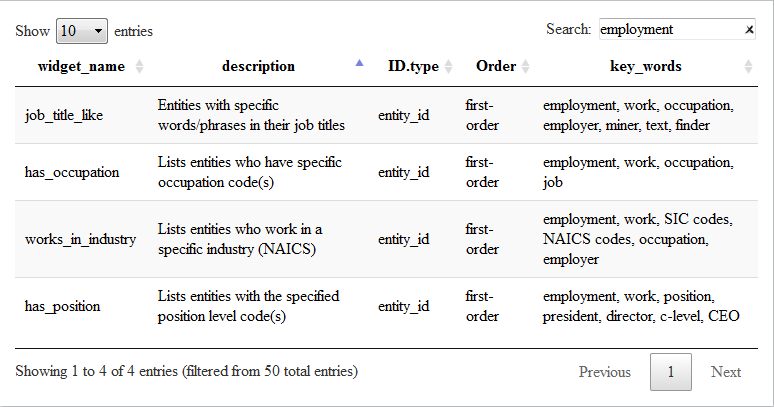
\includegraphics{images/show-widgets-employment.png}
\caption{Searching for widgets related to employment data}
\end{figure}

You can browse the entire listing, or use the search bar at the top right to search for specific widgets.

The second way to search for widgets is to use the \texttt{widget\_for} function. This function takes as an argument a search term, and finds all widgets that are related to that search term. For example:

\begin{Shaded}
\begin{Highlighting}[]
\KeywordTok{widget_for}\NormalTok{(}\StringTok{"giving"}\NormalTok{)}
\end{Highlighting}
\end{Shaded}

\begin{verbatim}
## fund_area:
##     Find funds with a particular area of giving code (type: allocation_code)
## fund_department:
##     Find funds with a particular department code (type: allocation_code)
## fund_miner:
##     Entities who gave to funds that match a keyword search (type: entity_id)
## fund_purpose:
##     Find funds with a particular fund purpose (type: allocation_code)
## fund_text_contains:
##     Funds with notes/biographies that contain the specified search string(s) (type: allocation_code)
## fund_type:
##     Find funds with a particular fund type code (type: allocation_code)
## gave_to_area:
##     Lists entities who gave to specific areas with minimum giving and specific date range (type: entity_id)
## gave_to_department:
##     Lists entities who gave to specific departments with minimum giving and specific date range (type: entity_id)
## gave_to_fund:
##     Entities who have given to specified funds (type: entity_id)
## gave_to_fund_type:
##     Entities who have given to specific types of funds (type: entity_id)
## gave_to_purpose:
##     Find donors to funds with a particular purpose (type: entity_id)
## has_philanthropic_affinity:
##     Lists entities with philanthropic affinity(ies) (type: entity_id)
## has_philanthropic_interest:
##     Lists entities with philanthropic interest(s) (type: entity_id)
\end{verbatim}

Once you've found the widget you're looking for, you can get additional information using R's built-in help system. Just type a question mark followed by the name of the widget, e.g.~\texttt{?gave\_to\_area}.

\hypertarget{working-with-autocomplete}{%
\section{Leveraging autocomplete}\label{working-with-autocomplete}}

As the previous section illustrates, there are a bewildering number of widgets available in the Discovery Engine. To make them a little easier to navigate, we've attached standard prefixes to the names of groups of widgets with related functionality. Since RStudio's autocomplete pops up suggestions along with documnetation as you type, typing a known prefix is a good way to quickly find and access a widget.

\begin{figure}
\centering
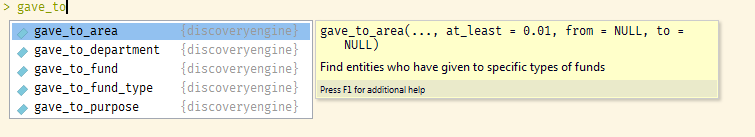
\includegraphics{images/gave-to-autocomplete.png}
\caption{Autocomplete pop up for giving widgets}
\end{figure}

Here are some of the groups of related widgets that use common prefixes in their names:

\begin{itemize}
\tightlist
\item
  Giving-related widgets: To find donors to the College of Natural Resources, you'd use \texttt{gave\_to\_area}. To find donors to scholarships, use \texttt{gave\_to\_purpose}. Type \texttt{gave\_to} and wait for a second to see the full list of giving widgets.
\item
  Political contribution widgets (federal): Widgets for \protect\hyperlink{ex-fec}{political contributions in federal elections} all begin with the prefix \texttt{fec\_}.
\item
  Political contribution widgets (statewide): Widgets for \protect\hyperlink{ex-ca-campaign}{political contributions in California elections} all begin with the prefix \texttt{ca\_}.
\end{itemize}

In addition to entity widgets, \protect\hyperlink{non-entity-widgets}{other types of widgets} are also helpfully grouped together.

\begin{itemize}
\tightlist
\item
  Every widget that pulls allocation codes instead of entity IDs begins with \texttt{fund\_} (for example, \texttt{fund\_type} or \texttt{fund\_department}).
\item
  Contact report widgets all begin with \texttt{contact\_} (for example \texttt{contact\_text\_contains} or \texttt{contact\_date}).
\item
  Proposal-based widgets all begin with \texttt{proposal\_} (for example, \texttt{proposal\_actual\_ask} or \texttt{proposal\_qualified}).
\end{itemize}

Finally, \texttt{bot\_brainstorm} and \texttt{bot\_matrix} are aliases for the \protect\hyperlink{brainstorm-bot}{\texttt{brainstorm\_bot}} and the \protect\hyperlink{matrix-bot}{\texttt{matrix\_bot}}, and in general, typing \texttt{bot\_} and waiting for a second will show a full list of the disco engine's bots.

\hypertarget{working-with-codes-synonyms}{%
\section{Codes and synonyms}\label{working-with-codes-synonyms}}

You may have noticed in previous examples that widgets work with exact codes, such as \texttt{in\_unit\_portfolio(BU)} or with \emph{synonyms}, such as \texttt{in\_unit\_portfolio(business)}. Synonyms will always be in lower-case, and may include any letter of the alphabet or the underscore "\_" character, and nothing else.

Use whichever feels more comfortable -- there is no advantage to using codes vs.~synonyms, though I personally find the synonyms easier to read and understand later on.

\hypertarget{synonym-search}{%
\section{Synonym search}\label{synonym-search}}

If you're not sure of the code or synonym to use, try out the synonym search feature that works with most widgets. Instead of entering a code (\texttt{in\_unit\_portfolio(BU)}) or synonym (\texttt{in\_unit\_portfolio(business)}), enter a question mark followed by a search string:

\begin{Shaded}
\begin{Highlighting}[]
\KeywordTok{in_unit_portfolio}\NormalTok{(?business)}
\end{Highlighting}
\end{Shaded}

\begin{verbatim}
## Regular codes and synonyms:
##   synonym code
##  business   BU
\end{verbatim}

You can enter partial terms:

\begin{Shaded}
\begin{Highlighting}[]
\KeywordTok{in_unit_portfolio}\NormalTok{(?sci)}
\end{Highlighting}
\end{Shaded}

\begin{verbatim}
## Regular codes and synonyms:
##                       synonym code
##   greater_good_science_center   GG
##  qb3_quantitative_biosciences   QB
##               letters_science   LS
##      lawrence_hall_of_science   LH
##        neuroscience_institute   NS
##           letters_and_science   LS
##                  neuroscience   NS
##       quantitative_bioscience   QB
##      quantitative_biosciences   QB
\end{verbatim}

And even multiple search terms:

\begin{Shaded}
\begin{Highlighting}[]
\KeywordTok{in_unit_portfolio}\NormalTok{(?bus, ?chem, ?public)}
\end{Highlighting}
\end{Shaded}

\begin{verbatim}
## Regular codes and synonyms:
##                        synonym code
##                       business   BU
##                      chemistry   CH
##                  public_health   PH
##                  public_policy   PP
##  communications_public_affairs   PA
\end{verbatim}

Widgets can always accept multiple codes/synonyms as arguments, and even combinations of the two:

\begin{itemize}
\tightlist
\item
  \texttt{gave\_to\_area(business)} would find anyone who has given to the school of Business
\item
  \texttt{gave\_to\_area(business,\ chemistry)} would find anyone who has given to Business or to Chemistry
\item
  \texttt{gave\_to\_area(HSB,\ COC)} is the same as above
\item
  \texttt{gave\_to\_area(business,\ COC)} once again, the same thing
\end{itemize}

\hypertarget{use-defaults}{%
\section{Use the default cases}\label{use-defaults}}

So by now you can probably figure out that \texttt{partcipated\_in(uc\_jazz\_ensembles)} gets you alumni who participated in the UC Jazz Ensembles. But what if you're actually looking for people who particpated in any student activity at all? Would you have to type out all (hundreds!) of them?

Luckily, no! In fact, all you have to do is type \texttt{participated\_in()}:

\begin{Shaded}
\begin{Highlighting}[]
\NormalTok{did_anything =}\StringTok{ }\KeywordTok{participated_in}\NormalTok{()}
\KeywordTok{display}\NormalTok{(did_anything)}
\end{Highlighting}
\end{Shaded}

\begin{verbatim}
## # A tibble: 256,802 x 1
##    entity_id
##        <dbl>
##  1         3
##  2         4
##  3         5
##  4         7
##  5         9
##  6        15
##  7        16
##  8        18
##  9        22
## 10        28
## # … with 256,792 more rows
\end{verbatim}

That seems a bit magical, doesn't it? The reason that works is because every widget has a defined behavior for when no codes/synonyms are entered. These default behaviors aim to be sensible so that you can use them in an intuitive way. You can always find out exactly what is included in the default by using the help. For instance, by typing \texttt{?has\_capacity} I find out that entering \texttt{has\_capacity()} without any specific ratings will find anyone with a researched capacity rating between 1 and 14 (so 99's are excluded, and those with no capacity ratings are excluded).

\hypertarget{widget-not-operator}{%
\section{\texorpdfstring{The \texttt{not()} operator}{The not() operator}}\label{widget-not-operator}}

Within a widget, you can use \texttt{not} to modify what you're looking for. For example, you can type \texttt{gave\_to\_fund\_type(not(endowment))} to find donors who gave to any kind of fund \textbf{other than} endowment funds. For an example of when this can be useful, see \protect\hyperlink{ex-mba-dual}{the MBA dual-degree holder example}.

\hypertarget{detailed-controls}{%
\section{Detailed controls}\label{detailed-controls}}

We saw above that \texttt{gave\_to\_area(business)} will find people who have given to the Haas School of Business. By default, this will find anyone who has ever given any amount, at any time. But \texttt{gave\_to\_area}, like many widgets, has a number of optional arguments that allow more fine-grained control. For example:

\begin{itemize}
\tightlist
\item
  \texttt{gave\_to\_area(business,\ at\_least\ =\ 10000)}: finds anyone who has given at least \$10,000 lifetime to the school of Business.
\item
  \texttt{gave\_to\_area(business,\ at\_least\ =\ 10000,\ from\ =\ 20160101)}: finds anyone who has given at least \$10,000 to Business since the beginning of 2016.
\item
  \texttt{gave\_to\_area(business,\ at\_least\ =\ 10000,\ from\ =\ 20150101,\ to\ =\ 20151231)}: finds anyone who gave at least \$10,000 to Business between January 1, 2015 and December 31, 2015.
\item
  \texttt{gave\_to\_area(business,\ from\ =\ 20150101,\ to\ =\ 20151231)}: finds anyone who gave anything at all to the school of Business between January 1, 2015 and December 31, 2015
\end{itemize}

As you can see, you can pick and choose which optional arguments you want to use. To find out all of the possible controls for a widget, use the built in help. For example, type \texttt{?gave\_to\_area}.

\hypertarget{combining-widgets}{%
\chapter{Combining widgets}\label{combining-widgets}}

As flexible as individual widgets are, they won't help you too much by themselves. What makes them really useful is that they can be combined. There are three ways to combine widgets:

\begin{itemize}
\tightlist
\item
  \texttt{\%and\%} will look for entities who satisfy both widgets
\item
  \texttt{\%or\%} will look for entities who satisfy at least one of two widgets
\item
  \texttt{\%but\_not\%} will look for entities who satisfy a widget but do not satisfy a second widget.
\end{itemize}

Some quick examples:

\texttt{gave\_to\_area(art\_museum)\ \%and\%\ gave\_to\_area(cal\_performances)} finds anyone who has given to \textbf{both} the Art Museum and Cal Performances.

\texttt{gave\_to\_area(art\_museum)\ \%or\%\ gave\_to\_area(cal\_performances)} finds anyone who has ever given to either the Art Museum or to Cal Performances. Note that this would include everyone who was found in the previous (\texttt{\%and\%}) example, as well as those who only gave to one or the other area.

\texttt{gave\_to\_area(art\_museum)\ \%but\_not\%\ gave\_to\_area(cal\_performances)} finds anyone who has given to the Art Museum but has not given to Cal Performances.

\hypertarget{example}{%
\section{Example}\label{example}}

You're working with a major gift officer in the School of Business who is surprised to find out that alumni have been giving \$15,000+ gifts in response to annual appeals, with no follow-up from major gift officers. She calls you up and says:

\begin{quote}
I need to a report on everyone who has given \$15,000 or more this year who isn't yet in a portfolio, and I need it right away!
\end{quote}

You could probably have a savedlist ready before she's even hung up the phone:

\begin{Shaded}
\begin{Highlighting}[]
\NormalTok{important_prospects =}\StringTok{ }
\StringTok{    }\KeywordTok{gave_to_area}\NormalTok{(business, }\DataTypeTok{at_least =} \DecValTok{15000}\NormalTok{, }\DataTypeTok{from =} \DecValTok{20160101}\NormalTok{) }\OperatorTok\StringTok{ }
\StringTok{    }\KeywordTok{in_unit_portfolio}\NormalTok{(business)}

\KeywordTok{display}\NormalTok{(important_prospects)}
\end{Highlighting}
\end{Shaded}

\begin{verbatim}
## # A tibble: 485 x 1
##    entity_id
##        <dbl>
##  1      2723
##  2      3923
##  3      5355
##  4      5671
##  5      5832
##  6      5833
##  7      8481
##  8     10980
##  9     11346
## 10     12789
## # … with 475 more rows
\end{verbatim}

\hypertarget{part-bots}{%
\part{Bots}\label{part-bots}}

\hypertarget{brainstorm-bot}{%
\chapter{The Brainstorm Bot}\label{brainstorm-bot}}

\begin{Shaded}
\begin{Highlighting}[]
\CommentTok{# as always, i have to make sure the disco engine is loaded}
\KeywordTok{library}\NormalTok{(discoveryengine)}
\end{Highlighting}
\end{Shaded}

At this point, you're pretty empowered to search through the database for all sorts of prospects, provided you know something about the codes in the database. Even if you don't know the exact code for, say, basketball, you can use the
\protect\hyperlink{synonym-search}{synonym search feature} because you know which widget to use:

\begin{Shaded}
\begin{Highlighting}[]
\KeywordTok{played_sport}\NormalTok{(?basketball)}
\end{Highlighting}
\end{Shaded}

\begin{verbatim}
## Regular codes and synonyms:
##              synonym code
##       basketball_men MABB
##  cal_basketball_club RSBK
##     basketball_women WABB
\end{verbatim}

But now imagine someone has asked you for a list of people interested in robotics. Where would that be coded? Perhaps in multiple places? How can you find out?

Enter the brainstorm bot. The brainstorm bot is a robot that is knowledgeable about the code tables in CADS. Let's ask it about robotics:

\begin{Shaded}
\begin{Highlighting}[]
\KeywordTok{brainstorm_bot}\NormalTok{(}\StringTok{"robotics"}\NormalTok{)}
\end{Highlighting}
\end{Shaded}

\begin{verbatim}
## attended_event 
##     9325: BARS 2017: Bay Area Robotics Symposium
##     8761: Silicon Valley Forum: Medical Robotics
## fec_gave_to_committee 
##     C00521765: LIQUID ROBOTICS INC POLITICAL ACTION COMMITTEE (LIQUID ROBOTICS PAC)
##     C00582767: CAMPAIGN FOR A FEDERAL ROBOTICS COMMISSION
## has_interest 
##     ROB: Robotics
## participated_in 
##     RENY: Robotics & Engineering for Youth
##     ENRO: Cal Robotics
## sec_filed 
##     1409269: Restoration Robotics, Inc.
##     1528557: Corindus Vascular Robotics, Inc.
##     1409269: Restoration Robotics Inc
\end{verbatim}

Hey brainstorm bot, thanks for the ideas! The results show the name of a widget, along with the codes that are of interest, along with their description from the CADS code tables, so you can decide if they are appropriate for your project. You can then copy and paste to build up the right population:

\begin{Shaded}
\begin{Highlighting}[]
\KeywordTok{display}\NormalTok{(}\KeywordTok{has_interest}\NormalTok{(ROB))}
\end{Highlighting}
\end{Shaded}

\begin{verbatim}
## # A tibble: 8 x 1
##   entity_id
##       <dbl>
## 1     24020
## 2    300717
## 3    470691
## 4    824520
## 5    836356
## 6   3104808
## 7   3368828
## 8   3447240
\end{verbatim}

If it turns out you agree with every one of the brainstorm bot's suggestions, then you don't even have to copy and paste, because (surprise!) the brainstorm bot is actually giving you a fully filled out widget:

\begin{Shaded}
\begin{Highlighting}[]
\CommentTok{# if i wanted robotics fans in the san francisco MSA}
\NormalTok{prospects =}\StringTok{ }\KeywordTok{brainstorm_bot}\NormalTok{(}\StringTok{"robotics"}\NormalTok{) }\OperatorTok
\StringTok{    }\KeywordTok{lives_in_msa}\NormalTok{(san_francisco)}
\KeywordTok{display}\NormalTok{(prospects)}
\end{Highlighting}
\end{Shaded}

\begin{verbatim}
## # A tibble: 37 x 1
##    entity_id
##        <dbl>
##  1     20288
##  2    290025
##  3    300717
##  4    349805
##  5    391263
##  6    398291
##  7    398320
##  8    415023
##  9    419351
## 10    442491
## # … with 27 more rows
\end{verbatim}

\hypertarget{search-features}{%
\section{Search features}\label{search-features}}

The brainstorm bot understands wildcards at the beginning and/or ending of your search term:

\begin{Shaded}
\begin{Highlighting}[]
\KeywordTok{brainstorm_bot}\NormalTok{(}\StringTok{"robot*"}\NormalTok{)}
\end{Highlighting}
\end{Shaded}

\begin{verbatim}
## attended_event 
##     8760: Robots on the Edge:Intelligent Machines
##     6724: Haas East Bay Chp Robotic Event 06-18-14
##     9325: BARS 2017: Bay Area Robotics Symposium
##     8761: Silicon Valley Forum: Medical Robotics
##     9431: SVF: Robots on the Edge
## fec_gave_to_committee 
##     C00596908: ROBOTECHNOLOGY INC C.R.
##     C00521765: LIQUID ROBOTICS INC POLITICAL ACTION COMMITTEE (LIQUID ROBOTICS PAC)
##     C00717249: RALLY ROBOT ZAPS AOC
##     C00582767: CAMPAIGN FOR A FEDERAL ROBOTICS COMMISSION
##     C00717074: RALLY ROBOT 2020
## has_interest 
##     ROB: Robotics
## participated_in 
##     UROB: Robotmedia Presents
##     RENY: Robotics & Engineering for Youth
##     ENRO: Cal Robotics
## sec_filed 
##     1409269: Restoration Robotics, Inc.
##     1528557: Corindus Vascular Robotics, Inc.
##     1409269: Restoration Robotics Inc
\end{verbatim}

It also will do multiple searches at once:

\begin{Shaded}
\begin{Highlighting}[]
\KeywordTok{brainstorm_bot}\NormalTok{(}\StringTok{"robot*"}\NormalTok{, }\StringTok{"data science"}\NormalTok{)}
\end{Highlighting}
\end{Shaded}

\begin{verbatim}
## attended_event 
##     8760: Robots on the Edge:Intelligent Machines
##     6724: Haas East Bay Chp Robotic Event 06-18-14
##     9325: BARS 2017: Bay Area Robotics Symposium
##     7643: Career Conn: Data Science
##     9533: Applied Data Science Forum
##     8761: Silicon Valley Forum: Medical Robotics
##     8341: Career Connections: Data Science
##     9431: SVF: Robots on the Edge
##     7565: UR NY LG Data Science Salon 10-27-16
## fec_gave_to_committee 
##     C00596908: ROBOTECHNOLOGY INC C.R.
##     C00521765: LIQUID ROBOTICS INC POLITICAL ACTION COMMITTEE (LIQUID ROBOTICS PAC)
##     C00717249: RALLY ROBOT ZAPS AOC
##     C00582767: CAMPAIGN FOR A FEDERAL ROBOTICS COMMISSION
##     C00717074: RALLY ROBOT 2020
## gave_to_department 
##     DT: Berkeley Institute for Data Science
## has_interest 
##     DAT: Data Science
##     ROB: Robotics
## has_philanthropic_interest 
##     DT: Berkeley Institute for Data Science
##     M1: Data Science Education Program
## majored_in 
##     250AM: Data Science
##     2E0: Master of Information & Data Science
##     2011: Applied Data Science Certificate
## participated_in 
##     UROB: Robotmedia Presents
##     HDSC: Haas Data Science Club
##     RENY: Robotics & Engineering for Youth
##     ENRO: Cal Robotics
## sec_filed 
##     1409269: Restoration Robotics, Inc.
##     1528557: Corindus Vascular Robotics, Inc.
##     1409269: Restoration Robotics Inc
\end{verbatim}

\hypertarget{matrix-bot}{%
\chapter{The Matrix Bot}\label{matrix-bot}}

\hypertarget{introduction}{%
\section{Introduction}\label{introduction}}

\begin{Shaded}
\begin{Highlighting}[]
\CommentTok{# as always, i have to make sure the disco engine is loaded}
\KeywordTok{library}\NormalTok{(discoveryengine)}
\end{Highlighting}
\end{Shaded}

The \protect\hyperlink{brainstorm-bot}{brainstorm bot} is powered by a simple text search of our code tables. It relies on your search term appearing in the description of a particular code. That's similar to the sort of search you might encounter on a library website that looks for exact text matches to your search term in the title and perhaps keywords associated with a book. But what if there are relevant facts about (for example) a student activity that are not captured in its name? As a concrete example, if your definition includes music majors, it's possible (depending on your goals) that you'd also want to take a look at people who had participated in the student group \href{http://cnmat.berkeley.edu/}{CNMAT}, which stands for ``Center for New Music and Audio Technologies.'' But how would you find that? The student activity code for CNMAT is \texttt{LSCN}, and the description that appears in the code table is ``CNMAT Users Group.''

We don't store longer descriptions or other metadata about student groups the way we do with allocations (which allows us to do \protect\hyperlink{searching-fund-text}{in-depth searches} of fund terms and biographies). The word ``music'' does not appear in the code table entry for CNMAT, and so this code would slip by both the \protect\hyperlink{synonym-search}{synonym search} and the \protect\hyperlink{brainstorm-bot}{Brainstorm Bot} search. Just when we're about to lose hope, enter the \textbf{Matrix Bot}.

\begin{figure}
\centering
\includegraphics{images/neo.gif}
\caption{Whoa}
\end{figure}

\hypertarget{what-it-is}{%
\section{What it is}\label{what-it-is}}

The Matrix Bot analyzes an existing Disco Definition and looks for additional codes that might be related. It's a good way to broaden your search when you're doing open-ended prospecting. If the Brainstorm Bot is like looking up a book in the card catalog, then the Matrix Bot is like walking through the stacks to the shelves where your book is located, and glancing at all of other books that have been shelved in the same general location.

Note that you have to provide it with a Disco Engine definition to start (unlike the Brainstorm Bot, which only requires one or more search terms).

\hypertarget{example-1}{%
\section{Example}\label{example-1}}

We're interested in finding musicians, so we start with music majors:

\begin{Shaded}
\begin{Highlighting}[]
\NormalTok{is_musician =}\StringTok{ }\KeywordTok{majored_in}\NormalTok{(music)}
\end{Highlighting}
\end{Shaded}

But, since this is an open-ended prospecting project, we call up the Matrix Bot to widen the net:

\begin{Shaded}
\begin{Highlighting}[]
\KeywordTok{matrix_bot}\NormalTok{(is_musician)}
\end{Highlighting}
\end{Shaded}

\begin{verbatim}
## attended_event 
##     3271: L&S Music Dept Welcome Back Event
##     774: Creation Reception
##     2803: Music Lib. Grndbrk. Cer.
##     4181: Discover Cal - Music Dept
## gave_to_department 
##     MUS: Music
##     JAZZ: Jazz Ensembles
##     YMP: Young Musicians Program
##     AH: Arts & Humanities
##     UCCE: Choral Ensembles
## has_affiliation 
##     UCUBE: University Baroque Ensemble
##     MLS1: Chamber Chorus
##     MLS2: University Chorus
##     MLS3: Symphony Orchestra
##     MUFMU: Friends of Music
##     RC29: CAA Octet Alumni Club
##     RC35: CAA Cal Band Alumni Association
## has_interest 
##     MUS: Music
## has_occupation 
##     2726: Musician/Singer
## majored_in 
##     579: Music
## participated_in 
##     LSCN: CNMAT Users Group
##     LSNM: Berkeley New Music Project
##     LSRE: Repercussions Music Journal
##     UMUC: Music Connection
##     MSJZ: UC Jazz Ensembles
##     URRR: Raza Recruitment & Retention Center
##     MSMB: UC Marching Band Member
##     MSCH: UC Choral Ensembles
\end{verbatim}

As you can see, the Matrix Bot discovered a number of additional avenues for prospecting! As with the \protect\hyperlink{brainstorm-bot}{Brainstorm Bot}, the Matrix Bot results are best thought of as suggestions for further research: not all of the suggestions will be helpful for your particular project, and the best way to proceed is to research and learn more about the codes it suggests, to see if they are relevant to your project.

\hypertarget{botstrapping}{%
\section{Botstrapping}\label{botstrapping}}

Recall that the brainstorm bot returns a valid Disco Engine definition (more precisely, it returns the result of combining all of its suggestions using \texttt{\%or\%}). While we don't often use that fact (it's much more common to find yourself copying/pasting from the brainstorm bot results to select the widgets you want to use), it does lend to itself to a nice trick. We can use the matrix bot on brainstorm bot results to quickly and effortlessly identify a number of prospecting options. For example, if we're prospecting for the Chicano Studies department, but don't have a great idea where to start:

\begin{Shaded}
\begin{Highlighting}[]
\CommentTok{# i use the wildcard * to search for both "chicano" and "chicana"}
\KeywordTok{matrix_bot}\NormalTok{(}\KeywordTok{brainstorm_bot}\NormalTok{(}\StringTok{"chican*"}\NormalTok{))}
\end{Highlighting}
\end{Shaded}

\begin{verbatim}
## attended_event 
##     5883: EI Chicano/Latino Graduation 5-1-03
##     5884: EI Chicano/Latino Graduation 5-1-04
##     5885: EI Chicano/Latino Graduation 5-1-05
##     5886: EI Chicano/Latino Graduation 5-1-06
##     5887: EI Chicano/Latino Graduation 5-1-07
##     5891: EI Chicano/Latino Graduation 5-1-12
##     8864: Chicano Latino Chap Summer Welcome Party
##     8865: Chicano Latino Chap Summer Welcome Party
##     8895: Chicano Latino Chap Summer Welcome Party
##     8896: Chicano Latino Chapter Noche de Osos
##     5882: EI Chicano/Latino Graduation 5-1-02
##     5889: EI Chicano/Latino Graduation 5-1-09
##     5890: EI Chicano/Latino Graduation 5-1-10
##     8420: Chicano Latino Chapter Noche de Osos
##     5348: EI Chicano Latino Graduation 5-15-2011
##     5888: EI Chicano/Latino Graduation 5-1-08
##     3231: Sandra Hare Welcome Rec.
##     4454: CAA Mento Chic/Lat Ptshp
##     9435: Student Welcome Reception
##     8237: All-UC Latino Career Networking Event
##     4867: L&S 10th Anniversary Ethnic Studies Libr
##     4310: Boalt La Raza Recept.
## ca_gave_to_candidate 
##     CA4219530495: LARA, RICARDO
##     CA1613744954: GUILLEN, ABEL
## fec_gave_to_candidate 
##     H2CA10145: HERNANDEZ, JOSE M
##     H2CA36439: RUIZ, RAUL DR.
## gave_to_department 
##     CHICANO: Chicano Studies Program
##     MSGC: Multiculture, Sex & Gender Ctrs
##     ETHNIC: Ethnic Studies
##     TRSP: Transfer/ReEntry/Parent Ctr
##     SAGE: SAGE Scholars Program
##     VCEIO: Equity & Inclusion: VC's Office
##     CLL: Campus Life/Leadership
##     SLC: Student Learning Center
##     CEEE: Educ Equity & Excellence Centers
##     CEP: Educational Partnerships Center
##     OGB: Order of the Golden Bear
##     SW: Social Welfare
## has_affiliation 
##     MA27: CAA Chicano/Latino Alumni Volunteer
##     RC15: CAA Chicanx Latinx Alumni Assoc Nor Cal
##     RC5: *CAA La Raza Alumni Club-Defunct
##     LSBSP: Biology Scholars Program
##     MA17: TAAP/KASP Scholarship Interviewer
##     MA5: CAA Student Recruitment/Outreach Pgm
##     RC11: *CAA Alumni Club Officer
##     MA30: TAAP/KASP Scholarship Reader
##     RC18: CAA Cal Alumni Los Angeles Chapter
## has_interest 
##     MEX: Mexican-American/Chicano Interest
##     USL: U.S. Latino Interests
##     LAT: Latin American Interests
## has_occupation 
##     2100: Social Svcs/Community Relation
## majored_in 
##     160: Chicano Studies
##     919: Spanish Option D: Hispanic
##     360: Ethnic Studies
##     907: Spanish Option C2: Latin American
##     498: Latin American Studies
##     9A1: Gender & Women's Studies
##     882: Spanish
##     045: American Studies
## participated_in 
##     EDCH: Chicano Latina Arch Stdnt Assn
##     LSCI: Chicano Studies Undergrad Assoc
##     LSCL: Chicano/Latino Political Sci Assoc
##     UCHE: Chicanxs/Latinxs in Health Education
##     UMEC: Movimiento Estud Chicano de Aztlan
##     GLTA: Lambda Theta Alpha Latin Sorority
##     UMAL: Mujeres Activas En Letras (MALCS)
##     UXIN: Xinaxtli
##     ULPL: Latino Pre-Law Society
##     ULV: La Voz
##     UTRE: TRENZA
##     GLTP: Lambda Theta Phi Latin Fraternity
##     UHAU: Hermanas Unidas
##     ULAS: Latin American Student Association
##     GLTN: Lambda Theta Nu Sorority
##     UHSF: Hispanic Scholarship Fund Scholars
##     UGFR: Grupo Folklorico Reflejos De Mexico
##     GGZA: Gamma Zeta Alpha
##     GSPA: Sigma Pi Alpha Sorority
##     UMCH: MEChXA
##     UHU: Hermanos Unidos
##     UDUL: DULCE-Cmnty Diabetes Educ & Prev
##     UYQU: Young Queers United 4 Empow (Y Que)
##     UEGI: Global Internship
##     ULF: La Familia
##     URRR: Raza Recruitment & Retention Center
##     RCRR: Raices Recruitment & Retention
##     GMGC: Multicultural Greek Council
##     URS: RISE-Rising Immigrant Sch Thru Educ
##     EIM: Casa Magdalena Mora
##     UESIT: Summer Abroad - Italy
##     UHES: Hispanic Engineers & Scientists
##     UIAM: IAM Outreach Program
##     UESMX: Summer Abroad - Mexico
##     BULS: Latino Business Student Association
##     ULL: La Llorona
##     UDCP: Destination: College Program
##     EAMEX: Education Abroad Program - Mexico
##     UBMC: Bridges Multicultural Resource Ctr
##     EID1: DC Advising Corps
##     EABRA: Education Abroad Program - Brazil
##     LBSIP: IRLE Labor Summer Internship Program
##     RHRV: Rochdale Village Co-Op Resident
##     LWLS: La Raza Law Students Association
##     LRAC: La Raza Alumni Chapter
##     EIP1: PDP Calculus Intensive
##     LTAD: Latino Alumni Directory
##     BIBSP: Biology Scholars Program
##     EIT: TAP Transfer Alliance Project
##     EISA: Educational Opportunity Program
##     USBR: Summer Bridge Program Participant
##     UBUI: BUILD Literacy Program
##     UBON: Bonner Leaders
##     EIR6: TRSP Transfer Student Services
##     LWLR: Berkeley La Raza Law Journal
##     UESSP: Summer Abroad - Spain
##     RHFW: Fenwick Weavers' Village Co-Op
## played_sport 
##     RSBX: Cal Boxing Club
## received_award 
##     ZFI: UA Zaffaroni Scholarship
##     CAS: CAA Achievement Award Scholar
##     IAS: Incentive Awards Scholar. Recipient
##     UEG: George A Miller Scholar
##     COS: Cal Opportunity Scholarship Recipient
\end{verbatim}

\hypertarget{how-does-it-work}{%
\section{How does it work?}\label{how-does-it-work}}

The Matrix Bot looks up entities who match your definition, and then looks for other characteristics they have in common. The theory is that if a lot of people who have characteristic A (example: majored in music) also happen to have characteristic B (participated in CNMAT Users Group), then there's probably an underlying similarity between characteristic A and B. This approach is closely related to one laid out in the paper \href{http://www.rci.rutgers.edu/~pmclean/mcleanp_01_920_313_breiger_duality.pdf}{``The Duality of Persons and Groups''} by Ronald Breiger.

The name ``Matrix Bot,'' in addition to evoking some \href{https://en.wikipedia.org/wiki/The_Matrix}{Neo-like magic}, is also a nod to the basic linear algebra that the bot uses.

\hypertarget{part-advanced}{%
\part{Advanced}\label{part-advanced}}

\hypertarget{higher-order-widgets}{%
\chapter{Higher order widgets}\label{higher-order-widgets}}

You may have noticed when we ran the \texttt{show\_widgets()} function in \protect\hyperlink{working-with-finding-widgets}{working with widgets} that there is a mysterious ``Order'' column that categorizes widgets as either ``first-order'' or ``second-order''. What's that all about? In order to answer that, let's take a look at another example.

\hypertarget{children-of-wealth}{%
\section{Children of wealth}\label{children-of-wealth}}

Many alumni in our database do not have capacity ratings, but come from wealthy families. This would be nice to be aware of if they were ever being solicited. But how could we identify these ``children of wealth'' using the discovery engine? It's pretty easy to find wealthy individuals:

\begin{Shaded}
\begin{Highlighting}[]
\CommentTok{# as always, i make sure the disco engine is loaded}
\KeywordTok{library}\NormalTok{(discoveryengine)}

\CommentTok{# i'll define wealthy as a capacity of $1 Million+}
\NormalTok{wealthy =}\StringTok{ }\KeywordTok{has_capacity}\NormalTok{(}\DecValTok{1}\OperatorTok{:}\DecValTok{7}\NormalTok{)}
\end{Highlighting}
\end{Shaded}

But now I'm stuck. I want to find children of anyone on that list. But so far all of the widgets we've seen work with specific codes, not other widgets. Technically, all the widgets we've seen are \emph{first-order} widgets. But we do have some widgets that, instead of working on one or more specific codes, works on an existing, already filled out widget. \texttt{child\_of} is one such \emph{second-order} widget:

\begin{Shaded}
\begin{Highlighting}[]
\NormalTok{child_of_wealth =}\StringTok{ }\KeywordTok{child_of}\NormalTok{(wealthy)}
\KeywordTok{display}\NormalTok{(child_of_wealth)}
\end{Highlighting}
\end{Shaded}

\begin{verbatim}
## # A tibble: 1,299 x 1
##    entity_id
##        <dbl>
##  1       155
##  2      1347
##  3      1529
##  4      2497
##  5      3181
##  6      3296
##  7      3308
##  8      3418
##  9      3442
## 10      3897
## # … with 1,289 more rows
\end{verbatim}

Though the syntax looks just like what we've been doing all along, note that \texttt{wealthy} in the above is not a code or synonym, but instead is the name that I gave to the definition \texttt{has\_capacity(1:7)}. This makes \texttt{child\_of} very different from other widgets we've seen so far. As we'll see in the next seciton, the ability to use second-order widgets allows us to do some very powerful things.

The result of using a second-order widget, though, is just like using any other widget. You can continue to combine it with other widgets:

\begin{Shaded}
\begin{Highlighting}[]
\KeywordTok{display}\NormalTok{(child_of_wealth }\OperatorTok\StringTok{ }\KeywordTok{lives_in_msa}\NormalTok{(san_francisco))}
\end{Highlighting}
\end{Shaded}

\begin{verbatim}
## # A tibble: 509 x 1
##    entity_id
##        <dbl>
##  1       155
##  2      1529
##  3      2497
##  4      3296
##  5      3418
##  6      3442
##  7      3897
##  8      4539
##  9      4540
## 10      5084
## # … with 499 more rows
\end{verbatim}

\begin{Shaded}
\begin{Highlighting}[]
\CommentTok{# or even}
\KeywordTok{display}\NormalTok{(}
    \KeywordTok{child_of}\NormalTok{(child_of_wealth)}
\NormalTok{)}
\end{Highlighting}
\end{Shaded}

\begin{verbatim}
## # A tibble: 148 x 1
##    entity_id
##        <dbl>
##  1     22266
##  2     22307
##  3     23574
##  4     25856
##  5     26067
##  6     27804
##  7     28003
##  8     28405
##  9     28586
## 10     28891
## # … with 138 more rows
\end{verbatim}

\hypertarget{non-entity-widgets}{%
\chapter{Non-entity widgets}\label{non-entity-widgets}}

\hypertarget{motivation}{%
\section{Motivation}\label{motivation}}

In CADSmart, there is a report called the Fundfinder, which allows you to search for allocations that contain specific words or phrases in the name, fund terms, or fund biography. A natural application is to use the report to find some allocations, and then turn around and get a list of entities who have given to those funds. So far, we haven't seen how to do that in the disco engine, but that's about to change. Before reading this section, make sure you understand \protect\hyperlink{higher-order-widgets}{higher order widgets}.

\hypertarget{non-entity-disco-definition-types}{%
\section{Disco Definition Types}\label{non-entity-disco-definition-types}}

Let's take a closer look at a widget we've already used a lot, the \texttt{has\_capacity} widget. In particular, let's look at the \protect\hyperlink{intro-example-create-def}{definition} that gets created when we use \texttt{has\_capacity}:

\begin{Shaded}
\begin{Highlighting}[]
\KeywordTok{has_capacity}\NormalTok{(}\DecValTok{1}\NormalTok{)}
\end{Highlighting}
\end{Shaded}

\begin{verbatim}
## LISTBUILDER DEFINITION (type: entity_id)
## .   source: d_entity_mv.entity_id (entity_id)
## .   logic: capacity_rating_code IN (1)
\end{verbatim}

See in parentheses in the first line where it says \texttt{type:\ entity\_id}? So \texttt{entity\_id} is the ``type'' of the definition we've created. And as you may have guessed by now, we can also create other types of definition!

\hypertarget{searching-fund-text}{%
\section{Searching fund text}\label{searching-fund-text}}

The Fundfinder report does not give you a list of entities, it gives you a list of allocations. You are then expected to use a different report to find donors to those allocations. We'll follow a similar (but hopefully more convenient) strategy with the disco engine. We start by using \texttt{fund\_text\_contains} to do a text search of fund terms/biographies/names (for more info, check the help file by typing \texttt{?fund\_text\_contains}). \texttt{fund\_text\_contains}, like all text-searching tools in the discoveryengine, allows you to enter as many search terms as you like, and to use wildcards (*):

\begin{Shaded}
\begin{Highlighting}[]
\CommentTok{# let's look for funds that support diversity/underrepresented students}
\NormalTok{diversity_funds =}\StringTok{ }\KeywordTok{fund_text_contains}\NormalTok{(}\StringTok{"divers*"}\NormalTok{, }\StringTok{"underrepresented"}\NormalTok{)}
\end{Highlighting}
\end{Shaded}

The definition looks pretty complex, but notice that first line -- this time around, instead of entity\_id, we have \texttt{type:\ allocation\_code}:

\begin{Shaded}
\begin{Highlighting}[]
\NormalTok{diversity_funds}
\end{Highlighting}
\end{Shaded}

\begin{verbatim}
## LISTBUILDER DEFINITION (type: allocation_code)
## .   operator (SZ29): union all
## .   left (SZ29): 
## .   .   source: f_allocation_mv.allocation_code (allocation_code)
## .   .   logic: regexp_like(long_name, '((^|\\s|\\W)divers)|((^|\\s|\\W)underrepresented($|\\s|\\W))', 'i')
## .   right (SZ29): 
## .   .   operator (AW42): union all
## .   .   left (AW42): 
## .   .   .   operator (QM15): union all
## .   .   .   left (QM15): 
## .   .   .   .   source: f_notes_mv.allocation_code (allocation_code)
## .   .   .   .   logic: 
## .   .   .   .   .   regexp_like(description, '((^|\\s|\\W)divers)|((^|\\s|\\W)underrepresented($|\\s|\\W))', 'i')
## .   .   .   .   .   note_type IN ('FT', 'FB')
## .   .   .   right (QM15): 
## .   .   .   .   source: f_notes_mv.allocation_code (allocation_code)
## .   .   .   .   logic: 
## .   .   .   .   .   regexp_like(brief_note, '((^|\\s|\\W)divers)|((^|\\s|\\W)underrepresented($|\\s|\\W))', 'i')
## .   .   .   .   .   note_type IN ('FT', 'FB')
## .   .   right (AW42): 
## .   .   .   source: f_notes_mv.allocation_code (allocation_code)
## .   .   .   logic: 
## .   .   .   .   regexp_like(note_text, '((^|\\s|\\W)divers)|((^|\\s|\\W)underrepresented($|\\s|\\W))', 'i')
## .   .   .   .   note_type IN ('FT', 'FB')
\end{verbatim}

And in fact, if we run \texttt{display}, we'll see a list of allocation codes instead of the entity IDs that we've seen in previous examples:

\begin{Shaded}
\begin{Highlighting}[]
\KeywordTok{display}\NormalTok{(diversity_funds)}
\end{Highlighting}
\end{Shaded}

\begin{verbatim}
## # A tibble: 294 x 1
##    allocation_code
##    <chr>          
##  1 R88958000      
##  2 R58436002      
##  3 R51943000      
##  4 R40872000      
##  5 FN1286000      
##  6 R48968000      
##  7 R57642000      
##  8 R50827000      
##  9 R45260000      
## 10 R91600000      
## # … with 284 more rows
\end{verbatim}

\hypertarget{from-funds-to-entities}{%
\section{From funds to entities}\label{from-funds-to-entities}}

If all you needed to do was get a list of allocation codes for your own research, then congrats, you're done! But what if you want to take the next step, and find donors to those funds? You use one of the \protect\hyperlink{working-with-finding-widgets}{tools to find widgets} to discover the \texttt{gave\_to\_fund} widget (read more at \texttt{?gave\_to\_fund}). Though it looks on the surface pretty similar to \texttt{gave\_to\_area} and \texttt{gave\_to\_department}, it is in fact one of those \protect\hyperlink{higher-order-widgets}{second-order widgets}!

\begin{Shaded}
\begin{Highlighting}[]
\CommentTok{# gave_to_fund has the same interface/options }
\CommentTok{# as gave_to_area and gave_to_department. }
\NormalTok{diversity_donors =}\StringTok{ }\KeywordTok{gave_to_fund}\NormalTok{(diversity_funds, }\DataTypeTok{at_least =} \DecValTok{10000}\NormalTok{,}
                                \DataTypeTok{from =} \DecValTok{20150101}\NormalTok{, }\DataTypeTok{to =} \DecValTok{20151231}\NormalTok{)}
\KeywordTok{display}\NormalTok{(diversity_donors)}
\end{Highlighting}
\end{Shaded}

\begin{verbatim}
## # A tibble: 31 x 1
##    entity_id
##        <dbl>
##  1       867
##  2     10469
##  3     12100
##  4     16607
##  5     21393
##  6     22653
##  7     23207
##  8     24473
##  9     27771
## 10     28097
## # … with 21 more rows
\end{verbatim}

\hypertarget{non-entity-converters}{%
\section{``Converters''}\label{non-entity-converters}}

Examples like this one show how higher-order widgets can act as ``converters,'' converting one type of definition (like \texttt{allocation\_code}) to another (like \texttt{entity\_id}). This is a handy idea to have in the back of your mind. If you find yourself with an ID list definition that has the wrong type of ID, see if you can find a second-order widget that will ``convert'' it to the right type.

\hypertarget{optional-arguments}{%
\chapter{Optional arguments}\label{optional-arguments}}

As we saw in \protect\hyperlink{detailed-controls}{Working with widgets}, many widgets have optional arguments that provide fine-grained control. You can always view the full documentation for a widget, including all of its arguments, by using the built-in help (e.g.~\texttt{?majored\_in}). We are able to make these arguments optional because widgets come pre-configured with default settings for these arguments (the default settings are also explained in the help).

\hypertarget{opt-events}{%
\section{Event invitees and attendees}\label{opt-events}}

For example, absent any additional instructions, \texttt{attended\_event} will exclude anyone who was invited but did not attend the specified events. So to create a definition of people who attended CNR's ``Re-discover ESPM'' event:

\begin{Shaded}
\begin{Highlighting}[]
\KeywordTok{attended_event}\NormalTok{(}\DecValTok{2770}\NormalTok{)}
\end{Highlighting}
\end{Shaded}

\begin{verbatim}
## LISTBUILDER DEFINITION (type: entity_id)
## .   source: d_bio_activity_mv.entity_id (entity_id)
## .   logic: 
## .   .   activity_code IN ('2770')
## .   .   activity_participation_code IN ('P', 'ST', 'SP', 'V', 'H', 'S', 'C', 'KN', 'MD', 'E', 'OL', 'IS')
\end{verbatim}

Since I did not specify otherwise, that definition will only pull in those who actually attended, not those who were merely invited. If I were interested not only in those who actually attended, but also anyone who was merely invited (this can be useful because it indicates that a person was at least considered an invite-worthy prospect), I would add \texttt{include\_non\_attendees\ =\ TRUE} to my specification:

\begin{Shaded}
\begin{Highlighting}[]
\KeywordTok{attended_event}\NormalTok{(}\DecValTok{2770}\NormalTok{, }\DataTypeTok{include_non_attendees =} \OtherTok{TRUE}\NormalTok{)}
\end{Highlighting}
\end{Shaded}

\begin{verbatim}
## LISTBUILDER DEFINITION (type: entity_id)
## .   source: d_bio_activity_mv.entity_id (entity_id)
## .   logic: 
## .   .   activity_code IN ('2770')
## .   .   activity_participation_code IN ('P', 'ST', 'SP', 'V', 'H', 'S', 'C', 'KN', 'MD', 'E', 'OL', 'IS', 'ID', 'RG', 'NS', 'RU')
\end{verbatim}

If you look closely at the printed output from each of those defintions, in the \texttt{logic} section, you'll notice slightly different lists of codes included where it says \texttt{activity\_participation\_code\ IN\ ...}. In fact, the latter includes the extra codes \texttt{ID} (for ``Invited but did not attend''), \texttt{RG} (``Regrets''), and \texttt{NS} (``No Show'').

\hypertarget{date-ranges}{%
\section{Date ranges}\label{date-ranges}}

A number of widgets, including all of the giving-related widgets as well as degree/major widgets, have two optional arguments, called \texttt{from} and \texttt{to}, to specify a date range. Their being optional means that you can specify none, just one, or both of the \texttt{from} and \texttt{to} arguments, resulting in the following behaviors:

\begin{itemize}
\tightlist
\item
  None: Dates will not be considered at all. So for example, \texttt{gave\_to\_area(chemistry)} will look at people's entire lifetime of giving for any gifts to the College of Chemistry
\item
  Only \texttt{from}: The date range will be considered open-ended on the right (future) side, but closed on the left (past). So \texttt{gave\_to\_area(chemistry,\ from\ =\ 20010101)} will look for anyone who has given to the College of Chemistry since the beginning of the year 2001, ignoring any giving that happened earlier than that.
\item
  Only \texttt{to}: The date range will be considered open-ended on the left (past), but closed on the right (future). So \texttt{gave\_to\_area(chemistry,\ to\ =\ 20080630)} will consider any giving on or before June 30, 2008, ignoring any giving that happened after that date.
\item
  Both: Just a daterange. \texttt{gave\_to\_area(chemistry,\ from\ =\ 20010101,\ to\ =\ 20080630)} will look for giving to the College of Chemistry between January 1, 2001 and June 30, 2008.
\end{itemize}

\hypertarget{graduate-undergraduate-attendee}{%
\section{Graduate, undergraduate, attendee}\label{graduate-undergraduate-attendee}}

For the most part, widgets have just a small number of options, and they are designed to be easy to get your head around. Should we include inactive records, yes or no? That kind of thing. Academic/degree-related widgets, including \texttt{majored\_in}, \texttt{has\_degree\_from}, \texttt{has\_degree}, and \texttt{minored\_in} have a somewhat more complex set of possibilites, arising from the fact that we can pull degreeholders, attendees, or current students, and graduates as well as undergraduates. We'll look at a couple of examples here, for more detailed explanations, \protect\hyperlink{ex-academic}{see the academic widgets example}:

\texttt{majored\_in(womens\_studies)}: By default, we look for both graduate and undergraduate degreeholders. Only those who completed a degree in Women's Studies will be included.

\texttt{majored\_in(womens\_studies,\ attendees\ =\ TRUE)}: By adding \texttt{attendees\ =\ TRUE}, we include any attendee, undergraduate or graduate, in addition to the degreeholders.

\texttt{majored\_in(womens\_studies,\ undergraduates\ =\ FALSE,\ current\_students\ =\ TRUE)}: Here we're only interested in graduate-level Women's Studies majors, including degreeholders and current students (but not attendees). We'll ignore undergraduate degreeholders as well as current undergraduate students. We'll include anyone who studied or is currently studying Women's Studies at the graduate level. Though it has the same meaning and will have the same results, in cases like this it's helpful to be explicit so you don't get confused later:

\begin{Shaded}
\begin{Highlighting}[]
\KeywordTok{majored_in}\NormalTok{(}
\NormalTok{    womens_studies,}
    \DataTypeTok{undergraduates =} \OtherTok{FALSE}\NormalTok{,}
    \DataTypeTok{graduates =} \OtherTok{TRUE}\NormalTok{, }\CommentTok{# not necessary (it's TRUE by default), but more clear}
    \DataTypeTok{current_students =} \OtherTok{TRUE}
\NormalTok{) }
\end{Highlighting}
\end{Shaded}

There are more examples using the academic widgets in \protect\hyperlink{ex-academic}{the examples gallery}.

\hypertarget{workarounds-inactive-only}{%
\section{Workarounds: inactive only}\label{workarounds-inactive-only}}

Sometimes the simplicity of a widget interface can make it seem insufficiently flexible. For example, what if we wanted to look at only people who were once in a library portfolio, but no longer are? By looking at \texttt{?in\_unit\_portfolio}, I can see that the unit portfolio widget has an option \texttt{include\_inactive} which is \texttt{FALSE} by default, but there is no \texttt{include\_active} or any such option. I can do \texttt{in\_unit\_portfolio(library,\ include\_inactive\ =\ TRUE)}, but that will include people who are still in a Library portfolio.

In order to get around this limitation, I'll have to get a little creative. I'll pull anyone in the library portfolio, whether active or inactive, but then I'll exclude those who are only in an active portfolio:

\begin{Shaded}
\begin{Highlighting}[]
\CommentTok{# first define what it means to have ever been in a library portfolio}
\NormalTok{current_or_former =}\StringTok{ }\KeywordTok{in_unit_portfolio}\NormalTok{(library, }\DataTypeTok{include_inactive =} \OtherTok{TRUE}\NormalTok{)}

\CommentTok{# now define being in a "current" portfolio}
\CommentTok{# note that include_inactive = FALSE is not necessary here, }
\CommentTok{# since that is the default setting for that argument, but }
\CommentTok{# i include it here because it makes my intent more clear}
\NormalTok{current =}\StringTok{ }\KeywordTok{in_unit_portfolio}\NormalTok{(library, }\DataTypeTok{include_inactive =} \OtherTok{FALSE}\NormalTok{)}

\CommentTok{# to find only the former portfolio:}
\NormalTok{former =}\StringTok{ }\NormalTok{current_or_former }\OperatorTok\StringTok{ }\NormalTok{current}
\end{Highlighting}
\end{Shaded}

This little trick is similar to the one we use in the \protect\hyperlink{ex-lybunt}{LYBUNT example}.

\hypertarget{part-related-tools}{%
\part{Related tools}\label{part-related-tools}}

\hypertarget{add-on-packages}{%
\chapter{Add-on packages}\label{add-on-packages}}

There are a growing number of packages that provide the Disco Engine user with additional functionality:

\hypertarget{discoappend}{%
\section{\texorpdfstring{\texttt{discoappend}}{discoappend}}\label{discoappend}}

\texttt{discoappend} allows you to output additional data (beyond just IDs) based on your disco engine definitions. For an introduction with examples, check \href{https://github.com/cwolfsonseeley/discoappend\#discoappend}{the official README}.

\hypertarget{discovcr}{%
\section{\texorpdfstring{\texttt{discovcr}}{discovcr}}\label{discovcr}}

\texttt{discovcr} allows you to browse data related to your discovery engine definition and select just the IDs you want to keep. This can be particularly useful when using text-search widgets such as \texttt{fund\_text\_contains}, where you may want to review the individual allocations you captured in your original search and remove any that were false matches (for example, a search for funds related to ``diversity'' brings in a number of biology research funds related to bio-diversity).

For a detailed introduction to using \texttt{discovcr}, read the ``vignette'' that includes examples and instructions by typing:

\begin{Shaded}
\begin{Highlighting}[]
\KeywordTok{vignette}\NormalTok{(}\StringTok{"vcr-intro"}\NormalTok{, }\DataTypeTok{package =} \StringTok{"discovcr"}\NormalTok{)}
\end{Highlighting}
\end{Shaded}

\hypertarget{discoscape}{%
\section{\texorpdfstring{\texttt{discoscape}}{discoscape}}\label{discoscape}}

The \texttt{discoscape} package serves as a bridge between the Discovery Engine and DonorScape. The \texttt{donorscape\_report} function outputs data in the format required by the DonorScape screening service, so that you can discover and/or define a population using the Discovery Engine, and then immediately run that population through a DonorScape without much hassle in between.

As with any package, you can load it up by using the \texttt{library} function:

\begin{Shaded}
\begin{Highlighting}[]
\KeywordTok{library}\NormalTok{(discoscape)}
\end{Highlighting}
\end{Shaded}

The main function is called \texttt{donorscape\_report}, and you can learn more about it by typing:

\begin{Shaded}
\begin{Highlighting}[]
\NormalTok{?donorscape_report}
\end{Highlighting}
\end{Shaded}

\hypertarget{part-examples}{%
\part{Examples}\label{part-examples}}

\hypertarget{ex-political-economy}{%
\chapter{Political economy list}\label{ex-political-economy}}

Here's the request:

\begin{quote}
Can you please generate a prospect list for me that includes econ, political economy, poli sci and business grads. And also include donors to Haas Center, Goldman School and CEGA?
\end{quote}

I start with the part I already know -- business grads.

\begin{Shaded}
\begin{Highlighting}[]
\KeywordTok{library}\NormalTok{(discoveryengine)}
\NormalTok{is_business_grad =}\StringTok{ }\KeywordTok{has_degree_from}\NormalTok{(business)}
\end{Highlighting}
\end{Shaded}

I believe Economics, Political Economy, and Political Science are all majors. I don't know major codes, but most widgets have a built-in lookup feature:

\begin{Shaded}
\begin{Highlighting}[]
\KeywordTok{majored_in}\NormalTok{(?econ)}
\end{Highlighting}
\end{Shaded}

\begin{verbatim}
## Regular codes and synonyms:
##                          synonym   code
##           agricultural_economics    024
##    household_arts_home_economics   373X
##                   law_jd_econ_ma 501246
##           pol_econ_of_indust_soc    697
##        pol_econ_of_nat_resources    698
##  agricultural_resource_economics    034
##                        economics    246
##                  economics_ma_jd 246501
##                political_economy    2B2
##        environmental_econ_policy    779
##          urban_secondary_english  24903
\end{verbatim}

Ok, looks like \texttt{economics} and \texttt{political\_economy} should definitely be included. What about political science?

\begin{Shaded}
\begin{Highlighting}[]
\KeywordTok{majored_in}\NormalTok{(?political)}
\end{Highlighting}
\end{Shaded}

\begin{verbatim}
## Regular codes and synonyms:
##            synonym code
##  political_economy  2B2
##  political_science  699
\end{verbatim}

So now I have what I need for the other graduates:

\begin{Shaded}
\begin{Highlighting}[]
\NormalTok{is_poli_econ_grad =}\StringTok{ }\KeywordTok{majored_in}\NormalTok{(political_science, political_economy, economics)}
\end{Highlighting}
\end{Shaded}

Now I need to find donors to the Haas Center, Goldman School, and CEGA. Some follow-up clarified that the ``Haas Center'' here is referring to the \href{http://haasinstitute.berkeley.edu/}{Haas Institute for a fair and inclusive society} . I don't know if that is an area of giving, a department, a fund? So I use the brainstorm bot. From experience, I know that ``institute'' sometimes appears in CADS as the full word ``institute'' and is sometimes abbreviated to something like ``inst.'' I'll use the wildcard (*) ability in the brainstorm bot to make sure I capture all possibilities:

\begin{Shaded}
\begin{Highlighting}[]
\KeywordTok{brainstorm_bot}\NormalTok{(}\StringTok{"haas inst*"}\NormalTok{)}
\end{Highlighting}
\end{Shaded}

\begin{verbatim}
## attended_event 
##     4340: Haas Institutional Analysis Workshop
##     2843: Haas Institutional Analysis Workshop
## has_affiliation 
##     BUA18: *Haas Inst of Mgmt, Innovation & Org
##     BUIBI: Haas Institute for Business Innovation
##     BUBSI: Haas Institute for Bus & Social Impact
## on_committee 
##     IBIAB: Haas Inst/Business Innovation Adv Board
\end{verbatim}

Ah ha! It's the department.

\begin{Shaded}
\begin{Highlighting}[]
\NormalTok{is_haas_ctr_donor =}\StringTok{ }\KeywordTok{gave_to_department}\NormalTok{(HDRC)}
\end{Highlighting}
\end{Shaded}

CEGA is the ``effective global action center.'' Once again, I'll ask the brainstorm bot for suggestions:

\begin{Shaded}
\begin{Highlighting}[]
\KeywordTok{brainstorm_bot}\NormalTok{(}\StringTok{"global action"}\NormalTok{)}
\end{Highlighting}
\end{Shaded}

\begin{verbatim}
## gave_to_department 
##     CEGA: Effective Global Action Center
## has_philanthropic_interest 
##     GA: Center for Effective Global Action
\end{verbatim}

\begin{Shaded}
\begin{Highlighting}[]
\NormalTok{is_cega_donor =}\StringTok{ }\KeywordTok{gave_to_department}\NormalTok{(CEGA)}
\end{Highlighting}
\end{Shaded}

I already happen to know that the Goldman School is an area of giving, so:

\begin{Shaded}
\begin{Highlighting}[]
\NormalTok{is_goldman_donor =}\StringTok{ }\KeywordTok{gave_to_area}\NormalTok{(public_policy)}
\end{Highlighting}
\end{Shaded}

The request was for people who meet any of the given criteria, so I'll use \texttt{\%or\%} to combine them:

\begin{Shaded}
\begin{Highlighting}[]
\NormalTok{prospect_list =}\StringTok{ }\NormalTok{is_business_grad }\OperatorTok\StringTok{ }
\StringTok{    }\NormalTok{is_poli_econ_grad }\OperatorTok
\StringTok{    }\NormalTok{is_haas_ctr_donor }\OperatorTok
\StringTok{    }\NormalTok{is_cega_donor }\OperatorTok
\StringTok{    }\NormalTok{is_goldman_donor}

\KeywordTok{display}\NormalTok{(prospect_list)}
\end{Highlighting}
\end{Shaded}

\begin{verbatim}
## # A tibble: 91,817 x 1
##    entity_id
##        <dbl>
##  1         2
##  2         5
##  3        13
##  4        16
##  5        28
##  6        51
##  7        78
##  8        81
##  9        98
## 10       109
## # … with 91,807 more rows
\end{verbatim}

\hypertarget{ex-lybunt}{%
\chapter{LYBUNTs}\label{ex-lybunt}}

\begin{Shaded}
\begin{Highlighting}[]
\CommentTok{# i always begin by loading the disco engine if it isn't already loaded}
\KeywordTok{library}\NormalTok{(discoveryengine)}
\end{Highlighting}
\end{Shaded}

Anyone involved in an annual solicitation cycle will have some interest in the population referred to as \emph{LYBUNT}, which stands for \textbf{L}ast \textbf{Y}ear \textbf{Bu}t \textbf{N}ot \textbf{T}his Year. That is, someone who gave last year but has not given this year. How can we create such a definition in the Disco Engine?

To make the example concrete, let's say we're identifying LYBUNTs for the school of Social Welfare. What I'd like to get to is:

\begin{Shaded}
\begin{Highlighting}[]
\NormalTok{LYBUNT =}\StringTok{ }\NormalTok{last_year }\OperatorTok\StringTok{ }\NormalTok{this_year}
\end{Highlighting}
\end{Shaded}

So, all I really need to do is define \texttt{last\_year} and \texttt{this\_year}. I'm writing this example in September, 2016, so I'll define ``last year'' as FY2015-16, or in other words, July 1, 2015 - June 30, 2016:

\begin{Shaded}
\begin{Highlighting}[]
\NormalTok{last_year =}\StringTok{ }\KeywordTok{gave_to_area}\NormalTok{(social_welfare, }\DataTypeTok{from =} \DecValTok{20150701}\NormalTok{, }\DataTypeTok{to =} \DecValTok{20160630}\NormalTok{)}
\end{Highlighting}
\end{Shaded}

And now for this year. Since the \texttt{to} argument is optional, I can just do:

\begin{Shaded}
\begin{Highlighting}[]
\NormalTok{this_year =}\StringTok{ }\KeywordTok{gave_to_area}\NormalTok{(social_welfare, }\DataTypeTok{from =} \DecValTok{20160701}\NormalTok{)}
\end{Highlighting}
\end{Shaded}

Now I can create my \texttt{LYBUNT} definition, as I strategized above:

\begin{Shaded}
\begin{Highlighting}[]
\NormalTok{LYBUNT =}\StringTok{ }\NormalTok{last_year }\OperatorTok\StringTok{ }\NormalTok{this_year}
\KeywordTok{display}\NormalTok{(LYBUNT)}
\end{Highlighting}
\end{Shaded}

\begin{verbatim}
## # A tibble: 186 x 1
##    entity_id
##        <dbl>
##  1       448
##  2       548
##  3      3408
##  4     10025
##  5     14061
##  6     14063
##  7     18578
##  8     22160
##  9     25099
## 10     30764
## # … with 176 more rows
\end{verbatim}

Finally, recall that \protect\hyperlink{use-defaults}{every widget has a default} set up if you don't enter any codes. Looking at \texttt{?gave\_to\_area} I can see that if I don't use an area of giving codes, I just get any giving anywhere. I can use this knowledge to get campus-wide LYBUNTs:

\begin{Shaded}
\begin{Highlighting}[]
\NormalTok{last_year =}\StringTok{ }\KeywordTok{gave_to_area}\NormalTok{(}\DataTypeTok{from =} \DecValTok{20150701}\NormalTok{, }\DataTypeTok{to =} \DecValTok{20160630}\NormalTok{)}
\NormalTok{this_year =}\StringTok{ }\KeywordTok{gave_to_area}\NormalTok{(}\DataTypeTok{from =} \DecValTok{20160701}\NormalTok{)}
\NormalTok{LYBUNT =}\StringTok{ }\NormalTok{last_year }\OperatorTok\StringTok{ }\NormalTok{this_year}
\KeywordTok{display}\NormalTok{(LYBUNT)}
\end{Highlighting}
\end{Shaded}

\begin{verbatim}
## # A tibble: 22,029 x 1
##    entity_id
##        <dbl>
##  1         7
##  2        15
##  3       202
##  4       225
##  5       340
##  6       515
##  7       533
##  8       601
##  9       620
## 10       814
## # … with 22,019 more rows
\end{verbatim}

\hypertarget{ex-recent-band-parents}{%
\chapter{Recent Band Parents}\label{ex-recent-band-parents}}

\begin{Shaded}
\begin{Highlighting}[]
\CommentTok{# always begin by loading the disco engine if it isn't already loaded}
\KeywordTok{library}\NormalTok{(discoveryengine)}
\end{Highlighting}
\end{Shaded}

A client in Student Affairs is considering organizing a weekend event for parents of marching band members who graduated recently. They are tentatively holding the event at the Claremont Resort, but want to be sure that there are enough recent band parents who live close enough to attend.

So our job is to build a definition of parents of recent band graduates who live near the Claremont Resort. Then we can just use \texttt{display} to view how many people fit the definition.

\hypertarget{recent-band-members}{%
\section{Recent band members}\label{recent-band-members}}

First I need to find out how to identify marching band members. I'll use the \protect\hyperlink{brainstorm-bot}{brainstorm bot}:

\begin{Shaded}
\begin{Highlighting}[]
\KeywordTok{brainstorm_bot}\NormalTok{(}\StringTok{"marching band"}\NormalTok{)}
\end{Highlighting}
\end{Shaded}

\begin{verbatim}
## participated_in 
##     MSMB: UC Marching Band Member
\end{verbatim}

Cool. So definining ``recent'' as anyone who graduated between 2010 and 2016:

\begin{Shaded}
\begin{Highlighting}[]
\NormalTok{recent_band_member =}\StringTok{ }\KeywordTok{participated_in}\NormalTok{(MSMB) }\OperatorTok
\StringTok{    }\KeywordTok{has_reunion_year}\NormalTok{(}\DecValTok{2010}\OperatorTok{:}\DecValTok{2016}\NormalTok{)}
\end{Highlighting}
\end{Shaded}

\hypertarget{find-their-parents}{%
\section{Find their parents}\label{find-their-parents}}

Since I'm already familiar with \protect\hyperlink{higher-order-widgets}{higher order widgets}, I know what to do here:

\begin{Shaded}
\begin{Highlighting}[]
\NormalTok{band_parent =}\StringTok{ }\KeywordTok{parent_of}\NormalTok{(recent_band_member)}
\end{Highlighting}
\end{Shaded}

\hypertarget{who-live-close-enough}{%
\section{Who live close enough}\label{who-live-close-enough}}

Here I'll assume that 25 miles is about as far as we can expect one of these band parents to travel in order to attend the event. So my definition should include only those people who live within 25 miles of the Claremont Resort:

\begin{Shaded}
\begin{Highlighting}[]
\NormalTok{event_prospect =}\StringTok{ }\NormalTok{band_parent }\OperatorTok\StringTok{ }
\StringTok{    }\KeywordTok{lives_near}\NormalTok{(}\StringTok{"Claremont Hotel and Spa"}\NormalTok{, }\DataTypeTok{miles =} \DecValTok{25}\NormalTok{)}
\end{Highlighting}
\end{Shaded}

\begin{verbatim}
## Basing results on: The Claremont Hotel, Claremont Avenue, Oakland, Alameda County, California, 94720-1076, United States of America (37.8594, -122.242)
\end{verbatim}

\hypertarget{how-many}{%
\section{How many?}\label{how-many}}

Now I just use \texttt{display} and see the number of parents:

\begin{Shaded}
\begin{Highlighting}[]
\KeywordTok{display}\NormalTok{(event_prospect)}
\end{Highlighting}
\end{Shaded}

\begin{verbatim}
## # A tibble: 147 x 1
##    entity_id
##        <dbl>
##  1     13799
##  2     14999
##  3     15672
##  4     15687
##  5     29578
##  6     46204
##  7     50302
##  8    229795
##  9    250310
## 10    271059
## # … with 137 more rows
\end{verbatim}

Notice the first line, before the IDs start, tells us exactly how many individuals are on the list: 147.

\hypertarget{householding}{%
\section{Householding}\label{householding}}

But hold up! Looking up some of these IDs, I'm noticing that both members of married couples are on the list. How many households are there here? I check the help for the \texttt{display} function by running \texttt{?display}. And I notice that there is an option called \texttt{household}, and by default it is set to \texttt{FALSE}. So:

\begin{Shaded}
\begin{Highlighting}[]
\KeywordTok{display}\NormalTok{(event_prospect, }\DataTypeTok{household =} \OtherTok{TRUE}\NormalTok{)}
\end{Highlighting}
\end{Shaded}

\begin{verbatim}
## # A tibble: 86 x 1
##    entity_id
##        <dbl>
##  1     13799
##  2     14999
##  3    229795
##  4    317956
##  5    347337
##  6    396274
##  7    766450
##  8    907499
##  9   3011819
## 10   3015961
## # … with 76 more rows
\end{verbatim}

\hypertarget{ex-near-builder}{%
\chapter{Nearing Builder of Berkeley Status}\label{ex-near-builder}}

\begin{Shaded}
\begin{Highlighting}[]
\CommentTok{# always begin by loading the disco engine if it isn't already loaded}
\KeywordTok{library}\NormalTok{(discoveryengine)}
\end{Highlighting}
\end{Shaded}

A household is designated a ``Builder of Berkeley'' when they have donated at least \$1 Million lifetime to Berkeley. That status comes with recognition and other perks, so it's valuable to be aware of households who are nearing that level, as we can then craft solicitations that would push the household into Builder status.

\hypertarget{defining-close}{%
\section{Defining close}\label{defining-close}}

For this example, I'll use \$850,000 as the definition of ``close'' to the \$1 Million Builder level. So we're trying to find households who have given at least \$850,000, but not over \$1 Million.

\protect\hyperlink{use-defaults}{Recall that} the giving widgets, when used without any area or department codes, look at giving anywhere on campus (which is what we want).

\begin{Shaded}
\begin{Highlighting}[]
\CommentTok{# B.O.B. is a lifetime recognition. Pull lifetime giving by not using the }
\CommentTok{# date range in the gave_to_area widget}
\NormalTok{nearly_builder =}\StringTok{ }\KeywordTok{gave_to_area}\NormalTok{(}\DataTypeTok{at_least =} \DecValTok{850000}\NormalTok{)}
\end{Highlighting}
\end{Shaded}

To exclude those who are already over \$1M (who are already Builders), I first need to identify them:

\begin{Shaded}
\begin{Highlighting}[]
\NormalTok{already_builder =}\StringTok{ }\KeywordTok{gave_to_area}\NormalTok{(}\DataTypeTok{at_least =} \DecValTok{1000000}\NormalTok{)}
\end{Highlighting}
\end{Shaded}

Now, I want to find everyone who satisfies \texttt{nearly\_builder} but are not \texttt{already\_builder}:

\begin{Shaded}
\begin{Highlighting}[]
\NormalTok{prospect_list =}\StringTok{ }\NormalTok{nearly_builder }\OperatorTok\StringTok{ }\NormalTok{already_builder}
\end{Highlighting}
\end{Shaded}

Let's see what we have!

\begin{Shaded}
\begin{Highlighting}[]
\KeywordTok{display}\NormalTok{(prospect_list)}
\end{Highlighting}
\end{Shaded}

\begin{verbatim}
## # A tibble: 78 x 1
##    entity_id
##        <dbl>
##  1       566
##  2      1306
##  3      3119
##  4      5832
##  5      5833
##  6      7318
##  7      8872
##  8     11724
##  9     15333
## 10     15771
## # … with 68 more rows
\end{verbatim}

\hypertarget{householding-1}{%
\section{Householding}\label{householding-1}}

A lot of individuals in \texttt{prospect\_list} are married to each other, but Builder of Berkeley is a household recognition. If I'm going to run the Prospect Pool Spreadsheet, this doesn't really matter since that report automatically households, but otherwise I'd like to household the results (this will also help in getting an accurate count). By checking \texttt{?display} I see that deceased people are removed by default (which is what I want in this case), but that householding is not done by default. To enable householding:

\begin{Shaded}
\begin{Highlighting}[]
\KeywordTok{display}\NormalTok{(prospect_list, }\DataTypeTok{household =} \OtherTok{TRUE}\NormalTok{)}
\end{Highlighting}
\end{Shaded}

\begin{verbatim}
## # A tibble: 47 x 1
##    entity_id
##        <dbl>
##  1     16759
##  2    363934
##  3    508590
##  4      1306
##  5      8872
##  6     15771
##  7    254804
##  8    653365
##  9    777368
## 10     23897
## # … with 37 more rows
\end{verbatim}

\hypertarget{ex-sim-donors}{%
\chapter{Donors who aren't degreeholders}\label{ex-sim-donors}}

\begin{Shaded}
\begin{Highlighting}[]
\CommentTok{# i always begin by loading the disco engine if it isn't already loaded}
\KeywordTok{library}\NormalTok{(discoveryengine)}
\end{Highlighting}
\end{Shaded}

We have what looks like an easy request:

\begin{quote}
Find donors to the School of Information who are not SIM degree holders.
\end{quote}

Having already looked up the codes, you immediately think:

\begin{Shaded}
\begin{Highlighting}[]
\KeywordTok{gave_to_area}\NormalTok{(SIM) }\OperatorTok\StringTok{ }\KeywordTok{has_degree_from}\NormalTok{(LI)}
\end{Highlighting}
\end{Shaded}

Unfortunately, as you begin reviewing the results, you notice that you produced a list that includes spouses of degree holders who received credit for household gifts to SIM.

To get around the issue, use the \texttt{married\_to} widget (a \protect\hyperlink{higher-order-widgets}{higher-order widget}). Note the use of parentheses to ensure the correct interpretation:

\begin{Shaded}
\begin{Highlighting}[]
\NormalTok{alum =}\StringTok{ }\KeywordTok{has_degree_from}\NormalTok{(LI)}
\NormalTok{non_alum_donor =}\StringTok{ }
\StringTok{    }\KeywordTok{gave_to_area}\NormalTok{(SIM) }\OperatorTok
\StringTok{    }\NormalTok{(alum }\OperatorTok\StringTok{ }\KeywordTok{married_to}\NormalTok{(alum))}
\end{Highlighting}
\end{Shaded}

\hypertarget{ex-fec}{%
\chapter{Utilizing FEC disclosure data}\label{ex-fec}}

\begin{Shaded}
\begin{Highlighting}[]
\CommentTok{# i always begin by loading the disco engine if it isn't already loaded}
\KeywordTok{library}\NormalTok{(discoveryengine)}
\end{Highlighting}
\end{Shaded}

Prospect Analysis regularly screens various public data against CADS, including FEC disclosures. This data makes its way into some of our predictive models, but on occasion it is useful to use the data directly.

\hypertarget{basics}{%
\section{Basics}\label{basics}}

The Disco Engine provides the following FEC widgets:

\begin{itemize}
\tightlist
\item
  \texttt{fec\_gave\_to\_committee}
\item
  \texttt{fec\_gave\_to\_candidate}
\item
  \texttt{fec\_gave\_to\_category}
\end{itemize}

Since the names of all of these related widgets begin with the same prefix, they are easy to find using RStudio's auto-completion:

\begin{figure}
\centering
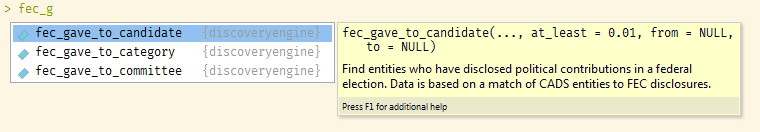
\includegraphics{images/fec-widgets-autocomplete.png}
\caption{just type ``fec\_''}
\end{figure}

The candidate and committee widgets should be pretty self-explanatory. \texttt{fec\_gave\_to\_category} is based on a categorization of PACs and other committees done by the \href{https://www.opensecrets.org/}{Center for Responsive Politics (opensecrets.org)}.

All of the widgets have the same interface as the giving widgets, meaning you can specify date ranges and minimum amounts when using them.

For example, to find donors to Kamala Harris's CA senate campaign who gave at least \$500 between January 1, 2016 and November 1, 2016:

\begin{Shaded}
\begin{Highlighting}[]
\KeywordTok{fec_gave_to_candidate}\NormalTok{(harris_kamala_d, }\DataTypeTok{at_least =} \DecValTok{500}\NormalTok{, }
                      \DataTypeTok{from =} \DecValTok{20160101}\NormalTok{, }\DataTypeTok{to =} \DecValTok{20161101}\NormalTok{)}
\end{Highlighting}
\end{Shaded}

As that example shows, the \protect\hyperlink{working-with-codes-synonyms}{system of codes and synonyms} works the same way with the FEC widgets as with any other widget. \protect\hyperlink{synonym-search}{Synonym search} is particularly useful with these widgets:

\begin{Shaded}
\begin{Highlighting}[]
\KeywordTok{fec_gave_to_category}\NormalTok{(?abortion)}
\end{Highlighting}
\end{Shaded}

\begin{verbatim}
## Regular codes and synonyms:
##                              synonym  code
##        abortion_policy_anti_abortion J7120
##  abortion_policy_pro_abortion_rights J7150
\end{verbatim}

\hypertarget{example-engineering-prospects}{%
\section{Example: Engineering Prospects}\label{example-engineering-prospects}}

A fundraiser might like to know if any of her prospects have recently made sizable political contributions:

\begin{Shaded}
\begin{Highlighting}[]
\CommentTok{# as with other widgets, leaving the committee code blank means i'm looking}
\CommentTok{# for giving to any committee}
\NormalTok{political_engineering_prospect =}\StringTok{ }
\StringTok{    }\KeywordTok{in_unit_portfolio}\NormalTok{(engineering) }\OperatorTok
\StringTok{    }\KeywordTok{fec_gave_to_committee}\NormalTok{(}\DataTypeTok{at_least =} \DecValTok{5000}\NormalTok{, }\DataTypeTok{from =} \DecValTok{20170101}\NormalTok{, }\DataTypeTok{to =} \DecValTok{20171031}\NormalTok{)}

\KeywordTok{display}\NormalTok{(political_engineering_prospect)}
\end{Highlighting}
\end{Shaded}

\begin{verbatim}
## # A tibble: 27 x 1
##    entity_id
##        <dbl>
##  1       616
##  2      5881
##  3     15333
##  4     16641
##  5     17677
##  6     21091
##  7     30551
##  8    130078
##  9    229827
## 10    283796
## # … with 17 more rows
\end{verbatim}

\hypertarget{example-environmental-interest}{%
\section{Example: Environmental Interest}\label{example-environmental-interest}}

We can use political giving to identify constituent interest in the environment. First, I'll use the lookup features to identify the right \texttt{category}:

\begin{Shaded}
\begin{Highlighting}[]
\KeywordTok{fec_gave_to_category}\NormalTok{(?environment)}
\end{Highlighting}
\end{Shaded}

\begin{verbatim}
## Regular codes and synonyms:
##                                      synonym  code
##                         environmental_policy JE300
##     energy_natural_resources_and_environment E0000
##  environmental_services_equipment_consulting E2000
\end{verbatim}

In this case, ``environmental policy'' is an ideological category, while the other two are industry PACs. Next, I might look for people who have expressed an interest in the environment by making political contributions to environmental policy organizations, but who have not already been coded with the

\begin{Shaded}
\begin{Highlighting}[]
\NormalTok{has_uncoded_environment_interest =}\StringTok{ }
\StringTok{    }\KeywordTok{fec_gave_to_category}\NormalTok{(environmental_policy) }\OperatorTok
\StringTok{    }\KeywordTok{has_interest}\NormalTok{(environment)}

\KeywordTok{display}\NormalTok{(has_uncoded_environment_interest)}
\end{Highlighting}
\end{Shaded}

\begin{verbatim}
## # A tibble: 2 x 1
##   entity_id
##       <dbl>
## 1   3178462
## 2   3178463
\end{verbatim}

\hypertarget{bots}{%
\section{Bots}\label{bots}}

Just like any other widget, FEC widgets are plugged in to the \protect\hyperlink{brainstorm-bot}{Brainstorm Bot} and \protect\hyperlink{matrix-bot}{Matrix Bot}. So, for instance:

\begin{Shaded}
\begin{Highlighting}[]
\KeywordTok{brainstorm_bot}\NormalTok{(}\StringTok{"cannabis"}\NormalTok{)}
\end{Highlighting}
\end{Shaded}

\begin{verbatim}
## fec_gave_to_category 
##     H4700: Pharmaceutical cannabis
## fec_gave_to_committee 
##     C00653444: CANNABIS SUPER PAC
##     C00675314: CITIZENS FOR THE LEGALIZATION OF CANNABIS POLITICAL ACTION COMMITTEE
##     C00718049: MAKE CANNABIS LEGAL AGAIN
##     C00681502: AMERICANS FOR CANNABIS NOW
##     C00569723: AMEICANS FOR CANNABIS LEGALIZATION
##     C00528026: NATIONAL CANNABIS INDUSTRY ASSOCIATION PAC
##     C00635896: CANNABIS COLLECTIVE
##     C00530683: AMERICANS FOR CANNABIS REFORM
##     C00662254: CANNABIS CATALYST POLITICAL ACTION COMMITTEE
##     C00647685: THE CANNABIS FUND
##     C00690149: CANNABIS TRADE FEDERATION ACTION FUND
##     C00534529: MEDICINAL CANNABIS SUPERPAC
##     C00628610: AMERICAN CANNABIS POLITICAL ACTION COMMITTEE
##     C00569723: AMERICANS FOR CANNABIS LEGALIZATION
##     C00613356: THE ACCC CANNABIS POLITICAL ACTION COMMITTEE
##     C00572545: MISSISSIPPI ALLIANCE FOR CANNABIS
##     C00534529: FEDERAL CANNABIS SUPERPAC
##     C00561159: SMART CANNABIS REFORM
## has_interest 
##     CAN: Cannabis
## participated_in 
##     UCBS: Cannabis Action Network
\end{verbatim}

Or:

\begin{Shaded}
\begin{Highlighting}[]
\KeywordTok{matrix_bot}\NormalTok{(}\KeywordTok{fec_gave_to_candidate}\NormalTok{(sanders_bernard))}
\end{Highlighting}
\end{Shaded}

\begin{verbatim}
## ca_gave_to_candidate 
##     CA3898358172: BOWEN, DEBRA
## fec_gave_to_candidate 
##     S4VT00033: SANDERS, BERNARD
##     H6OH23033: KUCINICH, DENNIS J
##     H6FL23063: CANOVA, TIMOTHY A.
##     H4IA03065: APPEL, STACI
##     H6MT01095: JUNEAU, DENISE
##     H4IA01077: VERNON, MONICA W
##     S8OK00233: RICE, ANDREW MONROE
##     H6NY19243: TEACHOUT, ZEPHYR
##     P40002545: KUCINICH, DENNIS J
##     S0AR00168: HALTER, WILLIAM A
##     H6WA07458: JAYAPAL, PRAMILA
##     H2CA06267: SOLOMON, NORMAN
##     H4IA04113: MOWRER, JIM
##     H6FL08213: GRAYSON, ALAN MARK
##     H6NH01230: SHEA-PORTER, CAROL
##     H4ME02200: CAIN, EMILY
##     S4IA00087: BRALEY, BRUCE L
##     S8WI00026: FEINGOLD, RUSSELL D
##     S0KY00123: CONWAY, JOHN WILLIAM (JACK)
##     H6CA44103: BARRAGAN, NANETTE
##     H4PA08116: NAUGHTON, SHAUGHNESSY
##     S4MI00355: PETERS, GARY
##     S6MD03458: EDWARDS, DONNA FERN
##     S4VT00017: LEAHY, PATRICK
##     S6MO00362: KANDER, JASON
##     S2NM00088: HEINRICH, MARTIN TREVOR
##     H0NH02181: KUSTER, ANN MCLANE
##     H8NV03036: TITUS, DINA
##     S6OH00254: STRICKLAND, TED
##     H6MN05183: ELLISON, KEITH MAURICE
##     H6WA08068: BURNER, DARCY
##     S8ME00080: ALLEN, THOMAS H
##     H4CA10075: EGGMAN, MICHAEL RAY
##     H2CA31125: AGUILAR, PETE
##     S8NV00156: ROSEN, JACKY
##     H6IL06141: DUCKWORTH, L. TAMMY
##     S8MN00438: FRANKEN, AL
##     S6NH00091: HASSAN, MARGARET WOOD
##     S2MA00170: WARREN, ELIZABETH
##     S6OH00163: BROWN, SHERROD
##     S8OR00207: MERKLEY, JEFFREY ALAN
##     S6MO00297: CARNAHAN, ROBIN
##     S6IL00292: DUCKWORTH, L TAMMY
##     S4KY00091: GRIMES, ALISON  LUNDERGAN
##     S8WA00194: CANTWELL, MARIA
##     S2WI00219: BALDWIN, TAMMY
##     S6NV00200: MASTO, CATHERINE CORTEZ
##     H2CA36439: RUIZ, RAUL DR.
##     S2CT00132: MURPHY, CHRISTOPHER S
##     S6IL00151: DURBIN, RICHARD J
##     S6RI00221: WHITEHOUSE, SHELDON II
##     S0MA00075: COAKLEY, MARTHA
##     S6PA00266: MCGINTY, KATHLEEN ALANA
##     H8CA09060: LEE, BARBARA
##     S2NV00209: BERKLEY, SHELLEY
##     S8FL00166: NELSON, BILL
##     S8NM00184: UDALL, TOM
##     S6MT00162: TESTER, JON
##     H2CA00120: BROWNLEY, JULIA
##     S0PA00434: SESTAK, JOSEPH A JR
##     S2ND00099: HEITKAMP, HEIDI
##     S0NH00219: SHAHEEN, JEANNE
##     S2WA00189: MURRAY, PATTY
##     S6MO00305: MCCASKILL, CLAIRE
##     S8NC00239: HAGAN, KAY R
##     S8AK00090: BEGICH, MARK
##     S8MI00281: STABENOW, DEBBIE
##     H8GA06195: OSSOFF, T. JONATHAN
##     P60007168: SANDERS, BERNARD
##     S8CO00172: UDALL, MARK E
##     P40002347: EDWARDS, JOHN
##     S0CO00211: BENNET, MICHAEL F
##     H0CA03078: BERA, AMERISH
##     S0AL00156: JONES, DOUG
##     H4CA11081: MCNERNEY, JERRY
## fec_gave_to_category 
##     Z1300: Third-Party Candidate Committees
##     J2300: Democratic officials, candidates & former members
##     JE300: Environmental policy
##     J2100: Democratic leadership PAC
##     J6100: Anti-Guns
##     J7150: Abortion policy/Pro-Abortion Rights
##     J7500: Minority/Ethnic Groups
##     J1200: Democratic/Liberal
##     J9000: Other single-issue or ideological groups
##     J7400: Women's issues
## gave_to_department 
##     PACS: Peace & Conflict Studies
##     EGP: Emma Goldman Papers Project
##     PFA: Pacific Film Archives
## has_interest 
##     POL: Politics
##     PCY: Public Policy
##     WOM: Women
##     DIV: Diverse Constituencies
\end{verbatim}

\hypertarget{ex-ca-campaign}{%
\chapter{Utilizing CA campaign finance data}\label{ex-ca-campaign}}

\begin{Shaded}
\begin{Highlighting}[]
\CommentTok{# i always begin by loading the disco engine if it isn't already loaded}
\KeywordTok{library}\NormalTok{(discoveryengine)}
\end{Highlighting}
\end{Shaded}

Prospect Analysis screens CADS data against campaign finance disclosures for California elections, as reported to the CA Secretary of State. The widgets to access this data are similar in form and function to the \protect\hyperlink{ex-fec}{FEC widgets}. They are:

\begin{itemize}
\tightlist
\item
  \texttt{ca\_gave\_to\_candidate}
\item
  \texttt{ca\_gave\_to\_proposition}
\item
  \texttt{ca\_gave}
\end{itemize}

The first two widgets only look at contributions in campaigns for statewide office. However, the Secretary of State's ``Cal Access'' database includes a number of transactions that don't fit into either of those two categories. For instance, contributions to a campaign for Superior Court Judge (who run locally, not statewide) or contributions to committees that are not directly affiliated with a single candidate/proposition (such as the Democratic State Central Committee of California). In order to be able to find any kind of contribution, use \texttt{ca\_gave}, which includes giving to statewide candidates and propositions as well as any other disclosed giving.

\hypertarget{example-state-senate-and-assembly-candidates}{%
\section{Example: State Senate and Assembly candidates}\label{example-state-senate-and-assembly-candidates}}

The UC Berkeley Foundation is holding an event which will feature appearances by State assembly member Phil Ting, former state senator and assembly member Holly Mitchell, and state senator (and former state assembly member) Jim Beall. In preparation for the event, they ask you to find out who among our constituents have contributed to these officials' campaigns when they were running for office and do some preliminary research on them. We start by identifying the candidate IDs for those candidates, using the same \protect\hyperlink{synonym-search}{synonym search} tool that works in every widget:

\begin{Shaded}
\begin{Highlighting}[]
\KeywordTok{ca_gave_to_candidate}\NormalTok{(?mitchell, ?ting, ?beall)}
\end{Highlighting}
\end{Shaded}

\begin{verbatim}
## Regular codes and synonyms:
##           synonym         code
##    mitchell_holly CA1223588942
##  mitchell_holly_j CA3479738832
##      ing_mitchell CA1065733190
##         ting_phil  CA657102211
##    keating_janice   CA15407672
##  keating_janice_e CA2583880518
##         beall_jim CA3663467903
\end{verbatim}

Once we know the correct candidate codes, we can pull contributors:

\begin{Shaded}
\begin{Highlighting}[]
\NormalTok{donors =}\StringTok{ }\KeywordTok{ca_gave_to_candidate}\NormalTok{(CA657102211, CA1223588942, CA3663467903)}
\KeywordTok{display}\NormalTok{(donors)}
\end{Highlighting}
\end{Shaded}

\begin{verbatim}
## # A tibble: 366 x 1
##    entity_id
##        <dbl>
##  1       331
##  2      1303
##  3      8666
##  4     11015
##  5     12306
##  6     12453
##  7     14259
##  8     15683
##  9     16251
## 10     16374
## # … with 356 more rows
\end{verbatim}

Just like giving and FEC widgets, the California campaign finance widgets all support the following optional arguments:

\begin{itemize}
\tightlist
\item
  \texttt{at\_least}: to find donors with total contributions over a specified amount. By default, this is assumed to be 1 cent.
\item
  \texttt{from} and \texttt{to}: to constrain the date range when looking for contributions. By default, all matched contributions will be searched regardless of date. Prospect Development's California campaign finance database goes back to 2006.
\end{itemize}

\hypertarget{propositions}{%
\section{Propositions}\label{propositions}}

The process for ballot propositions is pretty similar to the one for candidates, but with the added complication that donors to proposition campaigns can be either supporting or opposed to the proposition in question. An example will help illustrate.

If you're looking for prospects who are interested in public education, you might end up considering donors to propositions 30 (in the 2011-12 cycle) and 55 (in the 2015-15 cycle). Prop 30 raised taxes in order to pay for both public K-12 schools as well as community colleges, and Prop 55 extended those tax increases. Once again, we'll start with a \protect\hyperlink{synonym-search}{synonym search}:

\begin{Shaded}
\begin{Highlighting}[]
\KeywordTok{ca_gave_to_proposition}\NormalTok{(?education)}
\end{Highlighting}
\end{Shaded}

\begin{verbatim}
## Regular codes and synonyms:
##                                                                                   synonym
##                      kindergarten_university_public_education_facilities_bond_act_of_2004
##      ab_127_chapter_35_2006_nunez_education_facilities_kindergarten_university_public_edu
##  education_funding_real_property_parcel_tax_initiative_constitutional_amendment_and_statu
##                      sb_1174_chapter_753_statutes_of_2014_lara_english_language_education
##                      kindergarten_university_public_education_facilities_bond_act_of_2002
##                                                            education_funding_payment_plan
##                   tax_for_early_education_and_early_childhood_programs_initiative_statute
##      public_preschool_education_tax_increase_on_incomes_over_400000_for_individuals_80000
##          temporary_taxes_to_fund_education_guaranteed_local_public_safety_funding_initiat
##         tax_extension_to_fund_education_and_healthcare_initiative_constitutional_amendmen
##        code
##  BL20030055
##  BL2005001D
##  BL20050088
##  BL20150058
##  BL20010047
##  BL2009001B
##  BL20110038
##  BL20050082
##  BL20110030
##  BL20150055
\end{verbatim}

The \texttt{code} field looks at first like it is completely meaningless, but take a closer look at you might notice: the last 4 characters are the proposition number (e.g.~\texttt{0055}), while the 4 characters before that are the start of the election cycle that the proposition was a part of (so \texttt{2015} refers to the 2015-16 election cycle). So for this project, I'd use \texttt{BL20150055} and \texttt{BL20110030}. By default, \texttt{ca\_gave\_to\_proposition} will pull both supporters and oppononents of the propositions. While that may be useful if you're just looking for wealth indicators, you probably want to specify one or the other for any affinity-based work. So:

\begin{Shaded}
\begin{Highlighting}[]
\CommentTok{# to pull supporters of a tax increase to fund education:}
\NormalTok{tax_supporter =}\StringTok{ }\KeywordTok{ca_gave_to_proposition}\NormalTok{(BL20150055, BL20110030, }
                                       \DataTypeTok{support =} \OtherTok{TRUE}\NormalTok{)}

\CommentTok{# and opponents:}
\NormalTok{tax_opponent =}\StringTok{ }\KeywordTok{ca_gave_to_proposition}\NormalTok{(BL20150055, BL20110030, }
                                      \DataTypeTok{support =} \OtherTok{FALSE}\NormalTok{)}
\end{Highlighting}
\end{Shaded}

A quick glance at the \protect\hyperlink{matrix-bot}{Matrix Bot} results give us a good idea of which side of the political aisle these two groups are coming from:

\begin{Shaded}
\begin{Highlighting}[]
\KeywordTok{matrix_bot}\NormalTok{(tax_supporter)}
\end{Highlighting}
\end{Shaded}

\begin{verbatim}
## ca_gave_to_candidate 
##     CA545453741: DE LEON, KEVIN
##     CA3415765751: OSBORN, TORIE
##     CA3789174547: YEE, BETTY T.
##     CA580635557: PAVLEY, FRAN
##     CA2025703811: STERN, HENRY
##     CA165165894: TORLAKSON, TOM
##     CA1322715128: BECERRA, XAVIER
##     CA1664107145: YEE , BETTY T.
##     CA941720645: SKINNER, NANCY
## fec_gave_to_candidate 
##     H4CA21072: RENTERIA, AMANDA
##     H0CA33117: BASS, KAREN
##     H8CA10167: COX, TERRANCE JOHN (TJ)
##     S4MA00028: MARKEY, EDWARD JOHN MR
##     H2CA31125: AGUILAR, PETE
##     H2CA36439: RUIZ, RAUL DR.
##     H6AZ08038: GIFFORDS, GABRIELLE
##     H4CA10075: EGGMAN, MICHAEL RAY
##     H8NV03036: TITUS, DINA
##     S6OH00254: STRICKLAND, TED
##     H8CO04067: MARKEY, ELIZABETH HELEN
##     S2IN00091: DONNELLY, JOSEPH S
##     S6MO00362: KANDER, JASON
##     S4MI00355: PETERS, GARY
##     S8AK00090: BEGICH, MARK
##     H2CA43245: TAKANO, MARK
##     H2CA52089: PETERS, SCOTT
##     H8CA22089: CAPPS, LOIS
##     S8ME00080: ALLEN, THOMAS H
##     S6PA00100: SPECTER, ARLEN
##     H2CA26026: BERMAN, HOWARD L.
##     H2MA04073: KENNEDY, JOSEPH P III
##     H2CA00120: BROWNLEY, JULIA
##     H6CA04123: BROWN, CHARLES
##     S4GA11277: NUNN, MARY MICHELLE
##     S8CO00172: UDALL, MARK E
##     S2NM00088: HEINRICH, MARTIN TREVOR
##     S6NV00028: REID, HARRY
##     S6LA00227: LANDRIEU, MARY L
##     S6PA00266: MCGINTY, KATHLEEN ALANA
##     S2ND00099: HEITKAMP, HEIDI
##     S6VA00093: WARNER, MARK ROBERT
##     S8FL00166: NELSON, BILL
##     S8NY00082: SCHUMER, CHARLES E
##     S8NC00239: HAGAN, KAY R
##     S6NV00200: MASTO, CATHERINE CORTEZ
##     H0CA27085: SCHIFF, ADAM
##     S2VA00142: KAINE, TIMOTHY MICHAEL
##     S4NJ00185: BOOKER, CORY A
##     S2NV00209: BERKLEY, SHELLEY
##     H0CA10149: GARAMENDI, JOHN
##     S8NM00184: UDALL, TOM
##     H0CA03078: BERA, AMERISH
##     S0NH00219: SHAHEEN, JEANNE
##     H8CA05035: PELOSI, NANCY
##     S0CO00211: BENNET, MICHAEL F
##     S6NH00091: HASSAN, MARGARET WOOD
##     S6MO00305: MCCASKILL, CLAIRE
##     S8MI00281: STABENOW, DEBBIE
##     S6IL00292: DUCKWORTH, L TAMMY
##     H4CA11081: MCNERNEY, JERRY
##     S2WA00189: MURRAY, PATTY
##     S6MT00162: TESTER, JON
##     S6OH00163: BROWN, SHERROD
##     S8OR00207: MERKLEY, JEFFREY ALAN
##     S8WI00026: FEINGOLD, RUSSELL DANA
##     S0CA00199: FEINSTEIN, DIANNE
##     S8WA00194: CANTWELL, MARIA
##     S6CA00584: HARRIS, KAMALA D
##     S8MN00438: FRANKEN, AL
##     S2WI00219: BALDWIN, TAMMY
##     S0NY00410: GILLIBRAND, KIRSTEN ELIZABETH
##     S0AL00156: JONES, DOUG
##     S2CA00286: BOXER, BARBARA
##     S2MA00170: WARREN, ELIZABETH
## fec_gave_to_category 
##     J2100: Democratic leadership PAC
##     J7500: Minority/Ethnic Groups
##     Y0000: Unknown
##     J1200: Democratic/Liberal
## gave_to_department 
##     PP: Public Policy
##     CEEE: Educ Equity & Excellence Centers
## has_affiliation 
##     BLDR: Builders of Berkeley
## has_interest 
##     HUR: Human Rights
##     PCY: Public Policy
##     ENV: Environment
##     DIV: Diverse Constituencies
\end{verbatim}

\begin{Shaded}
\begin{Highlighting}[]
\KeywordTok{matrix_bot}\NormalTok{(tax_opponent)}
\end{Highlighting}
\end{Shaded}

\begin{verbatim}
## ca_gave_to_candidate 
##     CA1403064487: STRICKLAND, TONY
##     CA3516489204: POIZNER, STEVE
##     CA643204175: WHITMAN, MARGARET C.
##     CA4012945810: MC CLINTOCK, THOMAS
##     CA1728102410: BAKER, CATHARINE
##     CA4083971340: SCHWARZENEGGER, ARNOLD
## fec_gave_to_candidate 
##     S4AR00103: COTTON, THOMAS
##     H0CA10123: HARMER, DAVID
##     S0OH00133: PORTMAN, ROB
##     S0NV00138: ANGLE, SHARRON E
##     S2OH00170: MANDEL, JOSH
##     S0MA00109: BROWN, SCOTT P
##     S0SC00149: GRAHAM, LINDSEY OLIN
##     S0FL00338: RUBIO, MARCO
##     H2CA11135: GILL, RICKY
##     H6CA22125: MCCARTHY, KEVIN
##     S0CA00330: FIORINA, CARLY
##     H0OH08029: BOEHNER, JOHN A.
##     H8WI01024: RYAN, PAUL D.
##     S2CA00351: CAMPBELL, TOM
##     P80003353: ROMNEY, MITT / RYAN, PAUL D. 
##     P80002801: MCCAIN, JOHN S.
## fec_gave_to_category 
##     J1100: Republican/Conservative
##     J2200: Republican leadership PAC
##     Z4100: Republican Joint Candidate Committee
##     Z5100: Republican Party Committees
##     Z1100: Republican Candidate Committees
## has_interest 
##     VEN: Venture Capital
##     BUS: Business
##     REP: Republican Politics
\end{verbatim}

\hypertarget{ex-academic}{%
\chapter{Alumni and current students}\label{ex-academic}}

Several widgets in the Discovery Engine utilize degree information, including \texttt{has\_degree\_from}, \texttt{majored\_in}, \texttt{minored\_in}, and \texttt{has\_degree}. These widgets are set up to select undergraduate and graduate degreeholders, but have options to include or exclude attendees and current students as well. Because of the number of options available, these widgets may seem complex at first. These examples go over some of the more common cases.

Every degree/academic-related widget includes the following options for specifying degree status:

\begin{itemize}
\tightlist
\item
  \texttt{degreeholders}: whether to include (\texttt{TRUE}) or exclude (\texttt{FALSE}) degreeholders. By default, \texttt{degreeholders\ =\ TRUE}
\item
  \texttt{attendees}: include or exclude attendees -- these are people who attended UC Berkeley at some point (possibly just for one or two classes), but did not receive a degree. Defaults to \texttt{FALSE}
\item
  \texttt{current\_students}: include/exclude current students. Defaults to \texttt{FALSE}
\end{itemize}

They also include these options for specifying the level of attendance:

\begin{itemize}
\tightlist
\item
  \texttt{undergraduates}: whether to include (\texttt{TRUE}) or exclude (\texttt{FALSE}) undergraduate students/alumni. Defaults to \texttt{TRUE}
\item
  \texttt{graduates}: include or exclude graduate students/alumni. Defaults to \texttt{TRUE}
\end{itemize}

Finally, there are the options to specify dates, \texttt{from} and \texttt{to}. Dates are assumed to refer to when someone completed their stay at Berkeley (so the graduation date in the case of degreeholders, and the stop date for attendees). \texttt{from} and \texttt{to} are ignored when looking at current students.

It can be helpful to think of all the options in terms of a grid:

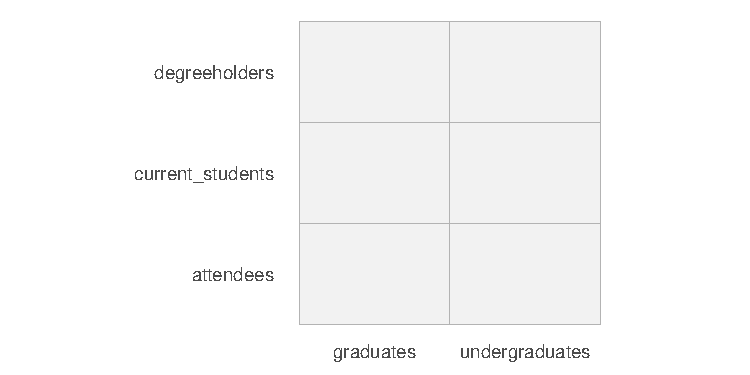
\includegraphics{images/unnamed-chunk-27-1.pdf}

By default, all academic widgets include only undergraduate and graduate degreeholders:
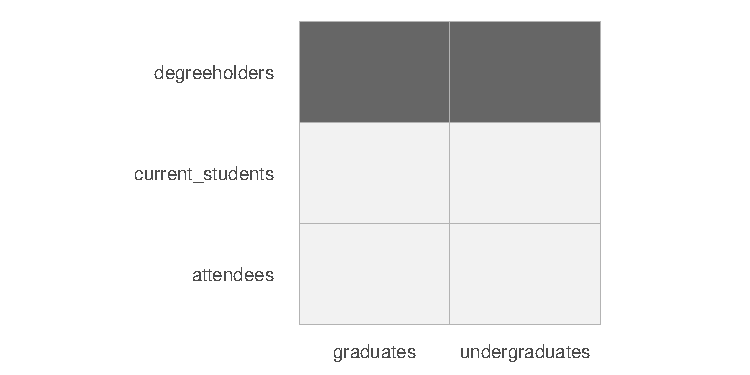
\includegraphics{images/unnamed-chunk-28-1.pdf}

Since those are the defaults, the code to get Chemistry degreeholders (undergraduate or graduate) is concise:

\begin{Shaded}
\begin{Highlighting}[]
\KeywordTok{has_degree_from}\NormalTok{(CH)}
\end{Highlighting}
\end{Shaded}

What if I only want undergraduate degreeholders?

\begin{Shaded}
\begin{Highlighting}[]
\KeywordTok{has_degree_from}\NormalTok{(CH, }\DataTypeTok{graduates =} \OtherTok{FALSE}\NormalTok{)}
\end{Highlighting}
\end{Shaded}

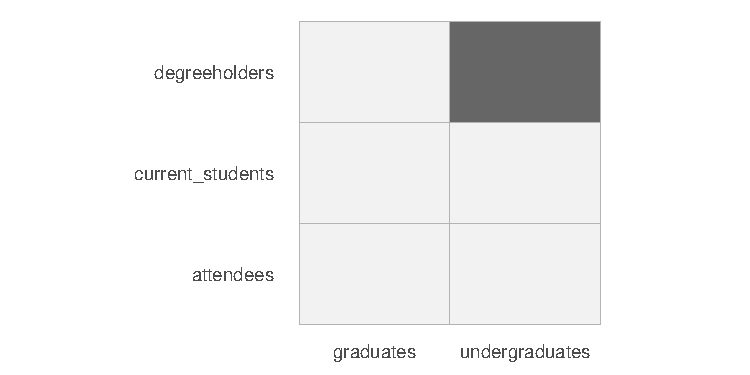
\includegraphics{images/unnamed-chunk-31-1.pdf}

\emph{Note: the reason I didn't have to type \texttt{undergraduates\ =\ TRUE} there is because that is the default. When in doubt, you always have the option of being explicit:}

\begin{Shaded}
\begin{Highlighting}[]
\KeywordTok{has_degree_from}\NormalTok{(CH, }\DataTypeTok{graduates =} \OtherTok{FALSE}\NormalTok{, }\DataTypeTok{undergraduates =} \OtherTok{TRUE}\NormalTok{)}
\end{Highlighting}
\end{Shaded}

When doing parents prospecting, it is common to need to look for current students.

\begin{Shaded}
\begin{Highlighting}[]
\KeywordTok{has_degree_from}\NormalTok{(CH, }
                \DataTypeTok{current_students =} \OtherTok{TRUE}\NormalTok{, }\DataTypeTok{degreeholders =} \OtherTok{FALSE}\NormalTok{, }
                \DataTypeTok{graduates =} \OtherTok{FALSE}\NormalTok{)}
\end{Highlighting}
\end{Shaded}

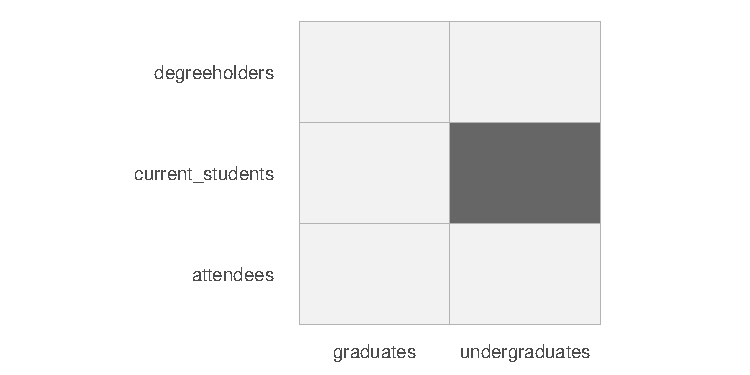
\includegraphics{images/unnamed-chunk-34-1.pdf}

\texttt{has\_degree\_from} searches based on school (Chemistry, Law, Letters \& Science, etc.), but other academic widgets have the same options and allow you to search based on major/minor or even the type of degree itself (e.g.~Ph.D., JD, Bachelor's, . . .). Here is how to get current MBA students:

\begin{Shaded}
\begin{Highlighting}[]
\KeywordTok{has_degree}\NormalTok{(MBA, }\DataTypeTok{current_students =} \OtherTok{TRUE}\NormalTok{, }\DataTypeTok{degreeholders =} \OtherTok{FALSE}\NormalTok{)}
\end{Highlighting}
\end{Shaded}

\hypertarget{ex-sec}{%
\chapter{Mining SEC filings}\label{ex-sec}}

\begin{Shaded}
\begin{Highlighting}[]
\CommentTok{# i always begin by loading the disco engine if it isn't already loaded}
\KeywordTok{library}\NormalTok{(discoveryengine)}
\end{Highlighting}
\end{Shaded}

The \href{https://www.sec.gov/}{SEC} is another one of the external data sources that Prospect Analysis regularly screens. Specifically, we utilize \href{https://www.sec.gov/fast-answers/answersform345htm.html}{SEC Form 3/4/5} filings made by our constituents. These filings are required of ``Corporate insiders -- meaning a company's officers and directors, and any beneficial owners of more than ten percent of a class of the company's equity securities,'' and are made whenever an individual first attains that status as a required filer, and then again every time the person buys or sells shares or derivatives in the company. The matched data is used in our predictive models as well as by the Prospect Discovery team, but it can also be valuable to be able to work with the data directly. (Note also that you can use the \texttt{screening} chunk in \texttt{discoappend} -- not demonstrated here -- in order to see summaries of all matched external data including SEC filings).

\hypertarget{basics-1}{%
\section{Basics}\label{basics-1}}

There is one SEC widget, called \texttt{sec\_filed}. This name keeps up the Disco Engine's convention of using a specific prefix to identify widgets that query matched external data (see also: \protect\hyperlink{ex-fec}{FEC widgets} and \protect\hyperlink{ex-ca-campaign}{California campaign widgets}). The most generic way to use the widget is without any arguments:

\begin{Shaded}
\begin{Highlighting}[]
\NormalTok{sec_filer =}\StringTok{ }\KeywordTok{sec_filed}\NormalTok{()}
\KeywordTok{display}\NormalTok{(sec_filer)}
\end{Highlighting}
\end{Shaded}

\begin{verbatim}
## # A tibble: 2,367 x 1
##    entity_id
##        <dbl>
##  1      2723
##  2      2937
##  3      3386
##  4      6194
##  5      6349
##  6      7011
##  7      7251
##  8      7270
##  9      7751
## 10      8002
## # … with 2,357 more rows
\end{verbatim}

The widget also includes the familiar \texttt{from} and \texttt{to} daterange options, so that you can search for people who made filings during a specific time period. For instance, my clients in Engineering might be interested in knowing who has made a recent filing, since these SEC filings can indicate a sudden influx of cash:

\begin{Shaded}
\begin{Highlighting}[]
\NormalTok{engineering_prospect =}\StringTok{ }\KeywordTok{in_unit_portfolio}\NormalTok{(engineering)}
\NormalTok{recent_filer =}\StringTok{ }\KeywordTok{sec_filed}\NormalTok{(}\DataTypeTok{from =} \DecValTok{20180101}\NormalTok{, }\DataTypeTok{to =} \DecValTok{20180630}\NormalTok{)}
\NormalTok{prospect_who_filed =}\StringTok{ }\NormalTok{engineering_prospect }\OperatorTok\StringTok{ }\NormalTok{recent_filer}
\KeywordTok{display}\NormalTok{(prospect_who_filed)}
\end{Highlighting}
\end{Shaded}

\begin{verbatim}
## # A tibble: 31 x 1
##    entity_id
##        <dbl>
##  1     14765
##  2     17517
##  3     17544
##  4     19406
##  5     25464
##  6     31155
##  7    122677
##  8    227268
##  9    283796
## 10    301895
## # … with 21 more rows
\end{verbatim}

\hypertarget{looking-for-companies}{%
\section{Looking for companies}\label{looking-for-companies}}

We use the \href{https://en.wikipedia.org/wiki/Central_Index_Key}{Central Index Key (CIK)} to uniquely identify SEC filers and the public companies for whom they work. Looking up a CIK in the Discovery Engine uses the familiar \protect\hyperlink{synonym-search}{lookup function} built in to widgets:

\begin{Shaded}
\begin{Highlighting}[]
\KeywordTok{sec_filed}\NormalTok{(?google, ?facebook, ?apple)}
\end{Highlighting}
\end{Shaded}

\begin{verbatim}
## Regular codes and synonyms:
##       synonym    code
##    google_inc 1288776
##  facebook_inc 1326801
##     apple_inc  320193
##     apple_inc  320193
\end{verbatim}

These IDs can then be used in the \texttt{sec\_filed} widget:

\begin{Shaded}
\begin{Highlighting}[]
\KeywordTok{display}\NormalTok{(}\KeywordTok{sec_filed}\NormalTok{(}\DecValTok{1288776}\NormalTok{, }\DecValTok{1326801}\NormalTok{, }\DecValTok{320193}\NormalTok{))}
\end{Highlighting}
\end{Shaded}

\begin{verbatim}
## # A tibble: 23 x 1
##    entity_id
##        <dbl>
##  1     22653
##  2     26031
##  3     26542
##  4    423075
##  5    423745
##  6    453623
##  7    611664
##  8    625613
##  9    666498
## 10    769804
## # … with 13 more rows
\end{verbatim}

\hypertarget{specific-roles}{%
\section{Specific roles}\label{specific-roles}}

The SEC filings include checkboxes for the filer to indicate which class of required filers (director, officer, ten percent owner, or other) she belongs to, and the \texttt{sec\_filed} widget has flags so that you can specifically search for people with these roles. For instance, if in my previous example I wanted to look only for Directors at those companies, I can set \texttt{director\ =\ TRUE}:

\begin{Shaded}
\begin{Highlighting}[]
\NormalTok{big_three_director =}\StringTok{ }\KeywordTok{sec_filed}\NormalTok{(}\DecValTok{1288776}\NormalTok{, }\DecValTok{1326801}\NormalTok{, }\DecValTok{320193}\NormalTok{, }\DataTypeTok{director =} \OtherTok{TRUE}\NormalTok{)}
\KeywordTok{display}\NormalTok{(big_three_director)}
\end{Highlighting}
\end{Shaded}

\begin{verbatim}
## # A tibble: 16 x 1
##    entity_id
##        <dbl>
##  1     22653
##  2     26031
##  3     26542
##  4    423075
##  5    423745
##  6    611664
##  7    625613
##  8    666498
##  9    769804
## 10    826016
## 11    863210
## 12    902313
## 13    921697
## 14    931282
## 15   3003117
## 16   3090604
\end{verbatim}

By default, all filings are included regardless of role.

Filers who check ``officer'' or ``other'' among their roles also have a free text entry space to more precisely describe their role with the company, and the \texttt{sec\_filed} includes an option to search the text of these fields. So, for example, to find people at one of the Big Three companies who've described themselves as ``Chairman'':

\begin{Shaded}
\begin{Highlighting}[]
\KeywordTok{sec_filed}\NormalTok{(}\DecValTok{1288776}\NormalTok{, }\DecValTok{1326801}\NormalTok{, }\DecValTok{320193}\NormalTok{, }\DataTypeTok{title_text =} \StringTok{"chairman"}\NormalTok{)}
\end{Highlighting}
\end{Shaded}

One practical use of the \texttt{title\_text} argument is to identify filers who were serving on an interim basis at the time of filing:

\begin{Shaded}
\begin{Highlighting}[]
\KeywordTok{display}\NormalTok{( }\KeywordTok{sec_filed}\NormalTok{(}\DataTypeTok{title_text =} \StringTok{"interim"}\NormalTok{) )}
\end{Highlighting}
\end{Shaded}

\begin{verbatim}
## # A tibble: 28 x 1
##    entity_id
##        <dbl>
##  1     15763
##  2     31278
##  3    232051
##  4    258787
##  5    268785
##  6    291703
##  7    330239
##  8    333051
##  9    348585
## 10    382348
## # … with 18 more rows
\end{verbatim}

\hypertarget{ex-mba-dual}{%
\chapter{Finding dual-degree holders}\label{ex-mba-dual}}

\begin{Shaded}
\begin{Highlighting}[]
\CommentTok{# i always begin by loading the disco engine if it isn't already loaded}
\KeywordTok{library}\NormalTok{(discoveryengine)}
\end{Highlighting}
\end{Shaded}

We recently received a request to take a look at Haas MBAs who have an additional degree from Berkeley, beyond their MBA. This was a tricky one. If we wanted to find people who have a joint MBA/MPH, we could just do:

\begin{Shaded}
\begin{Highlighting}[]
\KeywordTok{has_degree}\NormalTok{(MBA) }\OperatorTok\StringTok{ }\KeywordTok{has_degree}\NormalTok{(MPH)}
\end{Highlighting}
\end{Shaded}

But for this request, we want to find people with an MBA plus \textbf{any} other degree. We want to write something like:

\begin{Shaded}
\begin{Highlighting}[]
\KeywordTok{has_degree}\NormalTok{(MBA) }\OperatorTok\StringTok{ }
\StringTok{    }\KeywordTok{has_degree}\NormalTok{(any_other_degree_besides_mba)}
\end{Highlighting}
\end{Shaded}

How can we do that? Enter the \protect\hyperlink{widget-not-operator}{not operator}. Inside a widget, the \texttt{not()} operator excludes, rather than includes, the codes entered. So:

\begin{Shaded}
\begin{Highlighting}[]
\NormalTok{mba_dual_alum =}\StringTok{ }\KeywordTok{has_degree}\NormalTok{(MBA) }\OperatorTok\StringTok{ }
\StringTok{    }\KeywordTok{has_degree}\NormalTok{(}\KeywordTok{not}\NormalTok{(MBA))}

\KeywordTok{display}\NormalTok{(mba_dual_alum)}
\end{Highlighting}
\end{Shaded}

\begin{verbatim}
## # A tibble: 3,640 x 1
##    entity_id
##        <dbl>
##  1       137
##  2       159
##  3       217
##  4       235
##  5       252
##  6       257
##  7       311
##  8       340
##  9       358
## 10       513
## # … with 3,630 more rows
\end{verbatim}

\hypertarget{why-not-but_not}{%
\section{\texorpdfstring{Why not \texttt{\%but\_not\%}?}{Why not \%but\_not\%?}}\label{why-not-but_not}}

You might wonder, why do we need \texttt{not()} when we can combine widgets with \texttt{\%but\_not\%}? Our example will help illustrate the difference. This --

\begin{Shaded}
\begin{Highlighting}[]
\KeywordTok{has_degree}\NormalTok{(MBA) }\OperatorTok\StringTok{ }\KeywordTok{has_degree}\NormalTok{(MBA)}
\end{Highlighting}
\end{Shaded}

-- looks for anyone who both has an MBA degree and also does not have an MBA degree. Which is \href{https://en.wikipedia.org/wiki/Law_of_excluded_middle}{impossible}. What we did, on the other hand --

\begin{Shaded}
\begin{Highlighting}[]
\KeywordTok{has_degree}\NormalTok{(MBA) }\OperatorTok\StringTok{ }\KeywordTok{has_degree}\NormalTok{(}\KeywordTok{not}\NormalTok{(MBA))}
\end{Highlighting}
\end{Shaded}

-- looks for anyone who has an MBA degree as well as a non-MBA degree. And as we saw, there are thousands of such individuals.

\hypertarget{ex-moves-management}{%
\chapter{Moves Management}\label{ex-moves-management}}

\begin{Shaded}
\begin{Highlighting}[]
\CommentTok{# i always begin by loading the disco engine if it isn't already loaded}
\KeywordTok{library}\NormalTok{(discoveryengine)}
\end{Highlighting}
\end{Shaded}

The Discovery Engine provides a suite of widgets to identify proposals based on specific characteristics or events related to them.

\hypertarget{basics-2}{%
\section{Basics}\label{basics-2}}

With \protect\hyperlink{working-with-autocomplete}{autocomplete in mind}, proposal widgets are all prefixed with \texttt{proposal\_}.

\begin{figure}
\centering
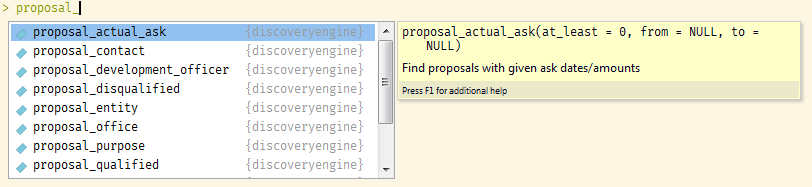
\includegraphics{images/proposal-autocomplete.png}
\caption{Common prefix keeps proposal widgets easy to find}
\end{figure}

As with all other widgets, the proposal widgets are designed to be combined like lego blocks using \texttt{\%and\%}, \texttt{\%or\%} and \texttt{\%but\_not\%} in order to precisely define solicitations (and planned solicitations) of interest. Once you've zeroed in on the proposals you're interested in, you can get the relevant enitity IDs using \texttt{proposal\_entity}, or look at related contact reports using \texttt{proposal\_contact}.

While these widgets can be used to pull the portfolio for a unit or development officer, it is simpler to use \texttt{in\_unit\_portfolio} and \texttt{in\_development\_officer\_portfolio} for those needs. The proposal widgets shine in situations where you need to focus on specific types of moves and asks, as the examples below illustrate.

\hypertarget{example-engineering-qualifications}{%
\section{Example: Engineering qualifications}\label{example-engineering-qualifications}}

Let's look for prospects who were qualified by Engineering during fiscal year 2017-18:

\begin{Shaded}
\begin{Highlighting}[]
\NormalTok{eng_qualification =}\StringTok{ }\KeywordTok{proposal_office}\NormalTok{(engineering) }\OperatorTok
\StringTok{    }\KeywordTok{proposal_qualified}\NormalTok{(}\DataTypeTok{from =} \DecValTok{20170701}\NormalTok{, }\DataTypeTok{to =} \DecValTok{20180630}\NormalTok{)}

\NormalTok{qualified_prospect =}\StringTok{ }\KeywordTok{proposal_entity}\NormalTok{(eng_qualification)}
\KeywordTok{display}\NormalTok{(qualified_prospect)}
\end{Highlighting}
\end{Shaded}

\begin{verbatim}
## # A tibble: 233 x 1
##    entity_id
##        <dbl>
##  1       235
##  2      1893
##  3      3422
##  4      6007
##  5      6945
##  6      7128
##  7     14661
##  8     16233
##  9     17719
## 10     21152
## # … with 223 more rows
\end{verbatim}

\texttt{proposal\_qualified} looks for proposals that moved from stage \texttt{QU} to one of \texttt{(CU,\ SP,\ PD,\ GS,\ DS)} during the specified time period (for a more flexible way to isolate specific types of moves, see \texttt{?proposal\_stage\_transition}). So our definition describes any proposal that successfully progressed from the qualification stage, during the fiscal year, that was assigned to Engineering at the time of the stage change.

\emph{Note: yes, the proposal widgets are smart enough to compare the assignment dates to the stage dates to make sure that the qualification really happened while the proposal was assigned to Engineering}

\hypertarget{example-collaborative-asks}{%
\section{Example: collaborative asks}\label{example-collaborative-asks}}

Which prospects were jointly solicited by the Library along with some other unit during fiscal year 2017-18? Let's focus only on asks of at least \$100,000. For this request, we'll take advantage of the \protect\hyperlink{widget-not-operator}{\texttt{not()} operator}:

\begin{Shaded}
\begin{Highlighting}[]
\NormalTok{joint_ask =}\StringTok{ }\KeywordTok{proposal_office}\NormalTok{(library) }\OperatorTok
\StringTok{    }\KeywordTok{proposal_office}\NormalTok{(}\KeywordTok{not}\NormalTok{(library)) }\OperatorTok
\StringTok{    }\KeywordTok{proposal_actual_ask}\NormalTok{(}\DataTypeTok{at_least =} \DecValTok{100000}\NormalTok{, }
                        \DataTypeTok{from =} \DecValTok{20170701}\NormalTok{, }\DataTypeTok{to =} \DecValTok{20180630}\NormalTok{)}

\NormalTok{jointly_asked =}\StringTok{ }\KeywordTok{proposal_entity}\NormalTok{(joint_ask)}
\KeywordTok{display}\NormalTok{(jointly_asked)}
\end{Highlighting}
\end{Shaded}

\begin{verbatim}
## # A tibble: 24 x 1
##    entity_id
##        <dbl>
##  1      1306
##  2     10864
##  3     15928
##  4     17429
##  5     23387
##  6     26209
##  7     38932
##  8     39287
##  9     39288
## 10     39794
## # … with 14 more rows
\end{verbatim}

\hypertarget{appendix-appendix}{%
\appendix}


\hypertarget{test-cdw}{%
\chapter{Test your database set up}\label{test-cdw}}

\hypertarget{test-your-connection}{%
\section{Test your connection}\label{test-your-connection}}

First, let's make sure your connection works. You'll need the user name and password you received when you got access to the data warehouse. Here are the steps to see if that connection works:

\begin{enumerate}
\def\labelenumi{\arabic{enumi})}
\tightlist
\item
  Navigate to C:\textbackslash Windows\textbackslash SysWOW64. Double click odbcad32. It's the application highlighted in the following image:
\end{enumerate}

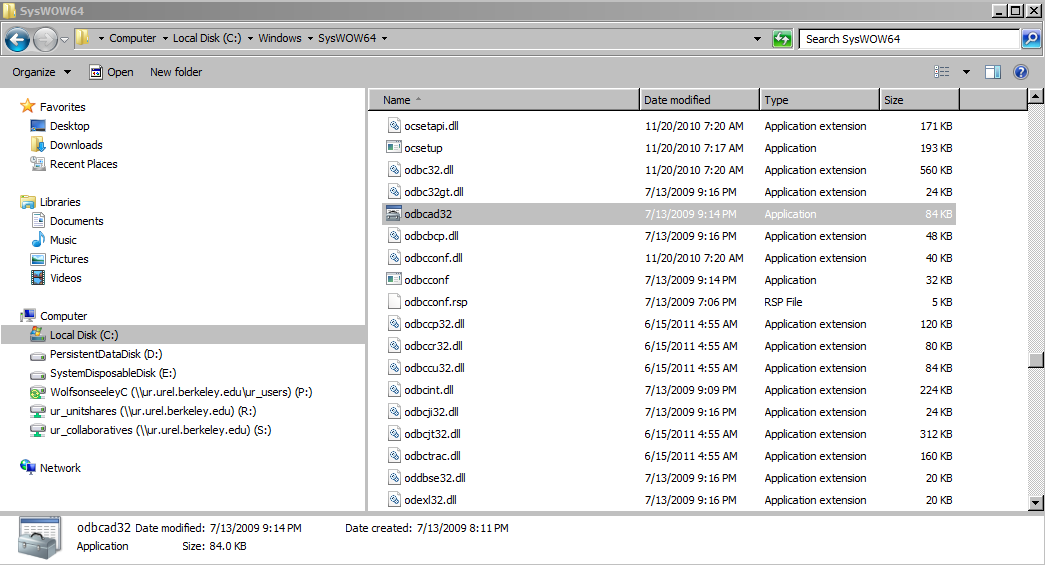
\includegraphics[width=15.67in]{images/syswow64}

\begin{enumerate}
\def\labelenumi{\arabic{enumi})}
\setcounter{enumi}{1}
\tightlist
\item
  You'll now have the ODBC Data Source Administrator open. Click the ``User DSN'' tab and then click the ``Add..'' button.
\end{enumerate}

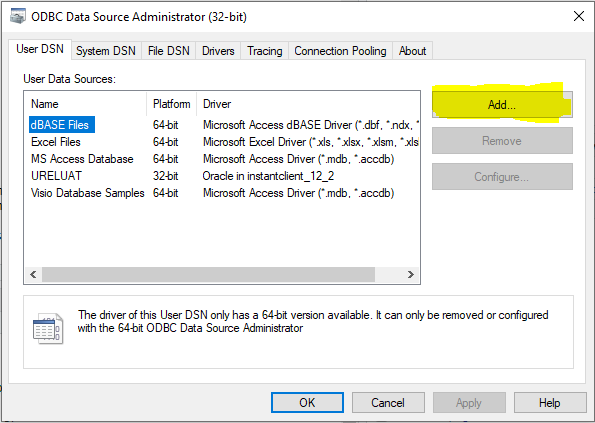
\includegraphics[width=8.26in]{images/odbc}

\begin{enumerate}
\def\labelenumi{\arabic{enumi})}
\setcounter{enumi}{2}
\tightlist
\item
  Scroll down to close to the bottom of the list of drivers. There you'll find ``Oracle in instantclient\_12\_2''. Double click this.
\end{enumerate}

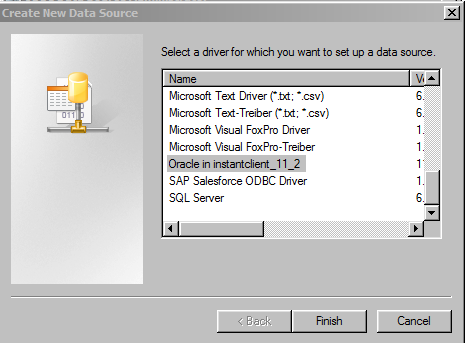
\includegraphics[width=6.5in]{images/oracle}

\begin{enumerate}
\def\labelenumi{\arabic{enumi})}
\setcounter{enumi}{3}
\tightlist
\item
  You'll now be in a window that asks you for some information to configure this driver. Fill out the Data Source Name as ``URELUAT'' and find ``URELUAT'' in the dropdown menu for TNS Service Name. Enter your user name (the one given to you by IST, which is probably the same as your CalNet ID) as the User ID. Click ``Test Connection''.
\end{enumerate}

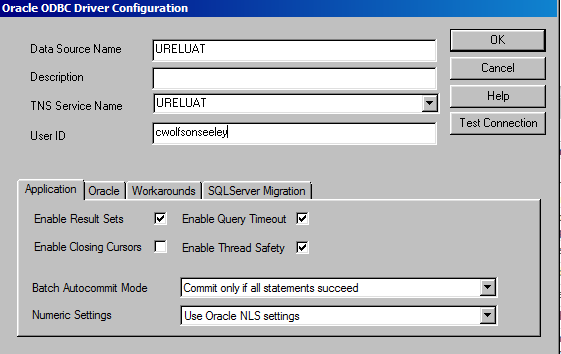
\includegraphics[width=7.82in]{images/configuration}

\begin{enumerate}
\def\labelenumi{\arabic{enumi})}
\setcounter{enumi}{4}
\tightlist
\item
  Enter your password (given to you by IST) in the Password field. Click ``OK''.
\end{enumerate}

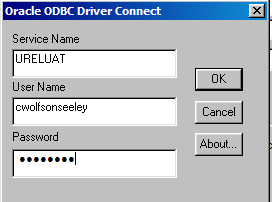
\includegraphics[width=3.71in]{images/test}

\begin{enumerate}
\def\labelenumi{\arabic{enumi})}
\setcounter{enumi}{5}
\tightlist
\item
  You should now get a pop up message letting you know that the connection was successful. Click ``OK'' three times to close out the ODBC Source Administrator. If you did not get this message and instead got an error message, do not continue with the rest of these instructions until your connection is successful. You may have the wrong password, or there may be other connection issues.
\end{enumerate}


\includegraphics[width=2.24in]{images/successful}

\hypertarget{opening-rstudio}{%
\section{Opening RStudio}\label{opening-rstudio}}

If your connection was successful, let's move on to making sure you can connect from within RStudio -- this will ensure that the Discovery Engine is able to query the data warehouse.

First, open RStudio. If you don't have an icon on your desktop, you can find the program by searching for ``rstudio'' in your Start menu. You'll also find a copy at C:\textbackslash Program Files\textbackslash RStudio\textbackslash bin. If you want a shortcut on your desktop, simply drag and drop the rstudio application.

When RStudio is open, you'll see a few different panes on the screen. The console is where you can type commands and see output. We only need to worry about the console right now. It's this part of the screen:

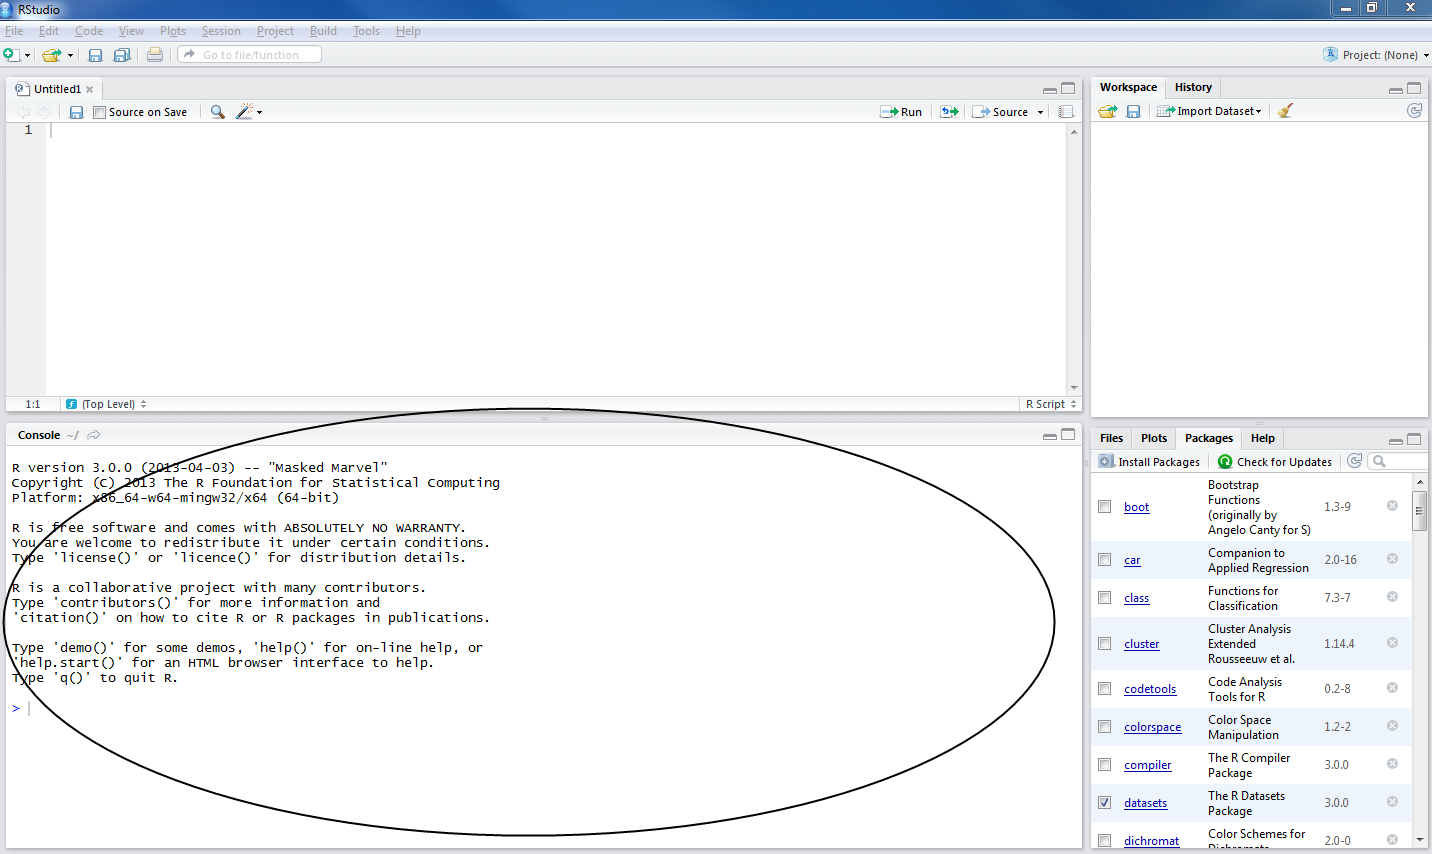
\includegraphics[width=21.33in]{images/console}

You also want to make sure you're using the correct version of R. Here are the steps to do so:

\begin{enumerate}
\def\labelenumi{\arabic{enumi})}
\tightlist
\item
  Go to the Tools dropdown menu at the top of the screen, and select Global Options. You'll see a box that looks like this:
\end{enumerate}

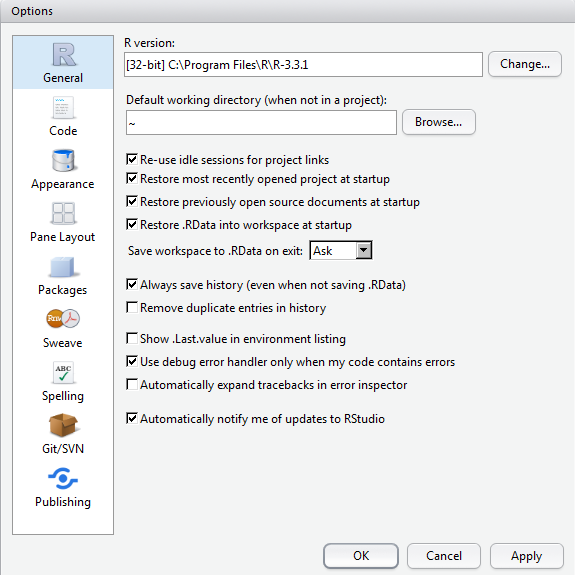
\includegraphics[width=8.18in]{images/options}

\begin{enumerate}
\def\labelenumi{\arabic{enumi})}
\setcounter{enumi}{1}
\tightlist
\item
  The top box tells you the R version you're using. Click on the ``Change..'' button. Then select the option that says ``Use your machine's default version of R (32-bit).'' Make sure it is 32-bit!
\end{enumerate}

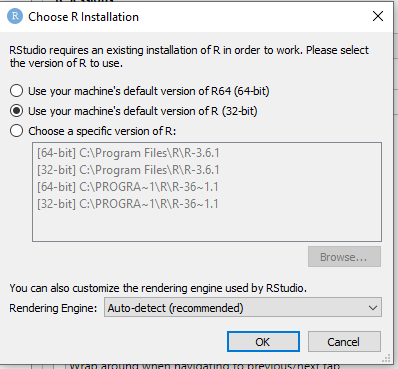
\includegraphics[width=5.53in]{images/version}

\begin{enumerate}
\def\labelenumi{\arabic{enumi})}
\setcounter{enumi}{2}
\tightlist
\item
  Click ``Ok'' twice. You may be prompted to restart the program. If so, go ahead and do so.
\end{enumerate}

\hypertarget{testing-getcdw}{%
\section{Testing getcdw}\label{testing-getcdw}}

Now we can run a test query from the data warehouse. Start by loading the library called \texttt{getcdw}:

\begin{Shaded}
\begin{Highlighting}[]
\KeywordTok{library}\NormalTok{(getcdw)}
\end{Highlighting}
\end{Shaded}

Copy the above into your console and press enter. It will appear that nothing happened, but that actually means everything is fine.

Now all we need to do is run a simple query to test the connection. We'll do this by entering a SQL query into the console and seeing if it returns valid data (which would mean that you are able to connect to the database). When you do so, you'll be prompted for some information, please read the instructions below and make sure you understand what you're supposed to enter:

\begin{Shaded}
\begin{Highlighting}[]
\KeywordTok{get_cdw}\NormalTok{(}\StringTok{"select * from dual"}\NormalTok{)}
\end{Highlighting}
\end{Shaded}

When you do this for the first time, you will be prompted for \emph{three} pieces of information:

\begin{enumerate}
\def\labelenumi{\arabic{enumi})}
\tightlist
\item
  Your ``UID'': This is your username to log-in to the database. Unless you were told otherwise, this should be the same as your CalNet ID.
\end{enumerate}

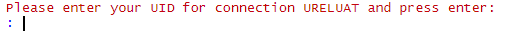
\includegraphics[width=7.24in]{images/UID}

\begin{enumerate}
\def\labelenumi{\arabic{enumi})}
\setcounter{enumi}{1}
\tightlist
\item
  Your ``PWD'': This is the password to log-in to the database. You will have received the password from IST and may be a random string of letters and numbers.
\end{enumerate}

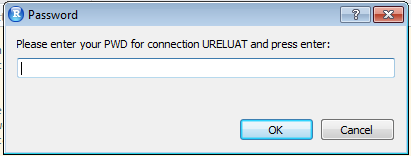
\includegraphics[width=5.61in]{images/PWD}

\begin{enumerate}
\def\labelenumi{\arabic{enumi})}
\setcounter{enumi}{2}
\tightlist
\item
  Finally, you'll be prompted for a ``secret passphrase.'' Instead of having you remember the password given to you by IST, getcdw allows you to pick your own secret passphrase (this can be anything, from a single word to a memorable sentence, or whatever you think is easy for you to remember but not easy for someone else to guess).
\end{enumerate}

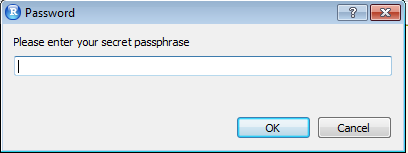
\includegraphics[width=5.67in]{images/passphrase}

After this step, you will only ever be required to enter your secret passphrase -- you will no longer be prompted for your database UID or PWD. (But you can always reset them if necessary, using reset\_credentials(dsn = ``URELUAT'').)

If everything is working properly, you should see something like this:

\begin{verbatim}
## # A tibble: 1 x 1
##   dummy
##   <chr>
## 1 X
\end{verbatim}

If that's what you see, you are all set!

\hypertarget{cheat-sheet}{%
\chapter{Cheat Sheet}\label{cheat-sheet}}

If you're looking for help installing the discovery engine, head over to the \href{https://cwolfsonseeley.github.io/discodocs/installation.html}{installation guide}. If you've previously installed the discovery engine, but need to update to the latest version, check the \href{https://cwolfsonseeley.github.io/discodocs/updating.html}{instructions for updating}.

\hypertarget{general}{%
\section{General}\label{general}}

\begin{itemize}
\tightlist
\item
  Always start a session with \texttt{library(discoveryengine)}
\end{itemize}

\begin{Shaded}
\begin{Highlighting}[]
\KeywordTok{library}\NormalTok{(discoveryengine)}
\end{Highlighting}
\end{Shaded}

\begin{itemize}
\tightlist
\item
  Use \texttt{show\_widgets()} for help \protect\hyperlink{working-with-finding-widgets}{finding the right widget}.
\item
  When in doubt, use the \protect\hyperlink{brainstorm-bot}{brainstorm bot}. For instance if you are looking for people who played on the basketball team, type \texttt{brainstorm\_bot("basketball")}
\item
  Multiple widgets \protect\hyperlink{combining-widgets}{can be combined} using the operators \texttt{\%and\%}, \texttt{\%or\%}, or \texttt{\%but\_not\%}.
\item
  Be aware of the \protect\hyperlink{add-on-packages}{add-on packages} for outputting additional data and improving your disco engine experience.
\item
  Use the documentation. For instance, type \texttt{?has\_affiliation} to understand how to use the \texttt{has\_affiliation} widget.
\end{itemize}

\hypertarget{output}{%
\section{Output}\label{output}}

Use \texttt{display} for output. Recall that you can use the equals sign \texttt{=} to assign names to your disco engine definitions, to make it easier to refer to them when \texttt{display}ing or doing other operations:

\begin{Shaded}
\begin{Highlighting}[]
\NormalTok{basketball_player =}\StringTok{ }\KeywordTok{played_sport}\NormalTok{(basketball_men, basketball_women)}
\KeywordTok{display}\NormalTok{(basketball_player)}
\end{Highlighting}
\end{Shaded}

\begin{verbatim}
## # A tibble: 489 x 1
##    entity_id
##        <dbl>
##  1       370
##  2      1495
##  3      3615
##  4      4425
##  5      5946
##  6      6412
##  7      6882
##  8      7539
##  9      8283
## 10      8328
## # … with 479 more rows
\end{verbatim}

If instead of just viewing IDs on the screen, you'd like to export them (perhaps to use in a CADS savedlist), just add a filename: \texttt{display(basketball\_player,\ file\ =\ "basketball-players")} and a file called ``basketball-players.csv'' will appear in your working directory. \emph{Note that the exported file has a header, so when you upload it to an Advance savedlist, make sure to check the ``First row is a header'' box.}

\hypertarget{code-lookup}{%
\section{Code lookup}\label{code-lookup}}

Most widgets rely on the coding found in CADS for their input, but you probably haven't memorized all of the codes! By using a question-mark inside of a widget, you can do look-ups on the fly:

\begin{Shaded}
\begin{Highlighting}[]
\KeywordTok{gave_to_department}\NormalTok{(?band)}
\end{Highlighting}
\end{Shaded}

\begin{verbatim}
## Regular codes and synonyms:
##   synonym    code
##  cal_band CALBAND
## 
## Defunct codes and synonyms:
##    synonym code
##  .cal_band  BAY
\end{verbatim}

Codes (such as \texttt{CALBAND}) and synonyms (such as \texttt{cal\_band}) can be used interchangeably, so use whichever feels more comfortable.

\hypertarget{text-search}{%
\section{Text search}\label{text-search}}

Though most widgets rely on codes from CADS as inputs, some utilize text search. Just like the \texttt{brainstorm\_bot}, which is also based on text search, these widgets require you to use quotation marks around the search term(s). Here are some examples:

\begin{itemize}
\tightlist
\item
  \texttt{contact\_text\_contains("neuro*",\ "brain")}
\item
  \texttt{fund\_text\_contains("diversity")}
\item
  \texttt{research\_miner("underrepresented")}
\end{itemize}

\textbf{Note:} The \texttt{brainstorm\_bot} will help you find things through the code tables, but it will not do big text searches of things like contact reports, fund biographies/terms, and research profiles. For that kind of specialized search, you should use these text search based widgets.

\hypertarget{other}{%
\section{Other}\label{other}}

Type \texttt{show\_suspect\_pools()} to view a list of all Suspect Pools, which is useful in conjunction with the \texttt{in\_suspect\_pool} widget.

\hypertarget{how-it-works}{%
\chapter{How does it work?}\label{how-it-works}}

In this section, I'll go over the basic building blocks that make the Disco Engine work. To help organize the lesson, I'll assume we're building a brand new Disco Engine from scratch. Of course, what we build will necessarily be just a simplified version of the Disco Engine, but we'll cover the most important concepts. All of the code behind the real Disco Engine is available for anyone to view \href{https://github.com/cwolfsonseeley/discoveryengine}{on GitHub}. Where possible, I'll add a link to the appropriate bit of production code and explain what's different from our simplified example.

\hypertarget{a-widget-as-a-sql-template}{%
\section{A Widget as a SQL template}\label{a-widget-as-a-sql-template}}

To get data from the database, the Disco Engine converts definitions into valid SQL. The key insight here is that any first-order predicate (\protect\hyperlink{higher-order-widgets}{what's first-order mean?}) can be represented in terms of a very basic SQL query, which we can turn into this all-purpose template:

\begin{Shaded}
\begin{Highlighting}[]
\KeywordTok{select} \KeywordTok{distinct}\NormalTok{ ID_FIELD }\KeywordTok{as}\NormalTok{ ID_TYPE}
\KeywordTok{from}\NormalTok{ TABLE_NAME}
\KeywordTok{where}\NormalTok{ FIELD_NAME }\KeywordTok{in}\NormalTok{ (LIST_OF_VALUES)}
\end{Highlighting}
\end{Shaded}

\emph{Note: The actual implementation allows for a broader range of queries, but this captures the basic idea. To see the actual templates used, check out \href{https://github.com/cwolfsonseeley/listbuilder/blob/master/R/templates.R}{the source code in the listbuilder package}}

There are a number of R packages that allow you to be able to construct templates this way and populate them with R objects. \texttt{discoveryengine} uses the \href{https://cran.r-project.org/web/packages/whisker/index.html}{whisker package}, but for this simplified example, I'll use \texttt{getcdw::parameterize\_template}:

\begin{Shaded}
\begin{Highlighting}[]
\KeywordTok{library}\NormalTok{(getcdw)}
\NormalTok{generate_query <-}\StringTok{ }\KeywordTok{parameterize_template}\NormalTok{(}\StringTok{"}
\StringTok{select distinct ##ID_FIELD## as ##ID_TYPE##}
\StringTok{from ##TABLE_NAME##}
\StringTok{where ##FIELD_NAME## in (##LIST_OF_VALUES##)}
\StringTok{"}\NormalTok{)}

\CommentTok{# generate_query is now a function with the same arguments as the }
\CommentTok{# names highlighted in the template}
\NormalTok{generate_query}
\end{Highlighting}
\end{Shaded}

\begin{verbatim}
## A parameterized template with parameters:  ID_FIELD, ID_TYPE, TABLE_NAME, FIELD_NAME, LIST_OF_VALUES
\end{verbatim}

Now, we can get a clunky, but functional, \texttt{has\_affiliation} widget working:

\begin{Shaded}
\begin{Highlighting}[]
\NormalTok{has_affiliation <-}\StringTok{ }\ControlFlowTok{function}\NormalTok{(affiliations) \{}
    \KeywordTok{list}\NormalTok{(}\DataTypeTok{ID_FIELD =} \StringTok{"entity_id"}\NormalTok{,}
         \DataTypeTok{ID_TYPE =} \StringTok{"entity_id"}\NormalTok{,}
         \DataTypeTok{TABLE_NAME =} \StringTok{"cdw.d_bio_affiliation_mv"}\NormalTok{,}
         \DataTypeTok{FIELD_NAME =} \StringTok{"affil_code"}\NormalTok{,}
         \DataTypeTok{LIST_OF_VALUES =} \KeywordTok{paste0}\NormalTok{(}\StringTok{"'"}\NormalTok{, affiliations, }\StringTok{"'"}\NormalTok{,}
                                \DataTypeTok{collapse =} \StringTok{", "}\NormalTok{))}
\NormalTok{\}}
\end{Highlighting}
\end{Shaded}

Wait, what? I wanted to create a constituency definition, but all I got was this lousy list!

\hypertarget{a-template-as-a-data-structure}{%
\section{A template as a data structure}\label{a-template-as-a-data-structure}}

Recall that definitions don't turn into IDs until we use the \texttt{display} function. The basic job of our \texttt{display} function will be to take care of two steps:

\begin{enumerate}
\def\labelenumi{\arabic{enumi}.}
\tightlist
\item
  Convert the definition (currently just a list) to SQL, and
\item
  Send the SQL to the database, returning the appropriate data
\end{enumerate}

So it makes sense that \texttt{has\_affiliation} just makes a list. It has all of the components of our definition, so we can inspect and figure out what it's supposed to return, but it won't actually return data from the data warehouse until we build a \texttt{display} function.

Luckily, step 2 of the \texttt{display} function is easy, because that's exactly what the function \texttt{getcdw::get\_cdw} does (if you're building for your own database, you just need a function here that can send SQL to your database and return a \texttt{data.frame}).

\begin{Shaded}
\begin{Highlighting}[]
\NormalTok{display <-}\StringTok{ }\ControlFlowTok{function}\NormalTok{(definition) \{}
    \KeywordTok{get_cdw}\NormalTok{(}\KeywordTok{to_sql}\NormalTok{(definition))}
\NormalTok{\}}
\end{Highlighting}
\end{Shaded}

How can we implement \texttt{to\_sql}? Well, that's just a matter of combining our template from \texttt{generate\_query} with the data to fill it in from \texttt{has\_affiliation}. The R function \texttt{do.call} lets us call any R function using a list of arguments. For example:

\begin{Shaded}
\begin{Highlighting}[]
\CommentTok{# here is the usual way we call a function:}
\CommentTok{# this takes 2 samples from the integers between 1 and 100}
\KeywordTok{sample}\NormalTok{(}\DataTypeTok{x =} \DecValTok{1}\OperatorTok{:}\DecValTok{100}\NormalTok{, }\DataTypeTok{size =} \DecValTok{2}\NormalTok{)}
\end{Highlighting}
\end{Shaded}

\begin{verbatim}
## [1] 12 89
\end{verbatim}

\begin{Shaded}
\begin{Highlighting}[]
\CommentTok{# but what if we've collected the arguments from some process?}
\NormalTok{args <-}\StringTok{ }\KeywordTok{list}\NormalTok{(}\DataTypeTok{x =} \DecValTok{1}\OperatorTok{:}\DecValTok{100}\NormalTok{, }\DataTypeTok{size =} \DecValTok{2}\NormalTok{)}

\CommentTok{# sample(args) won't work. what we want is do.call, which allows us to }
\CommentTok{# "feed" args as arguments to sample()}
\KeywordTok{do.call}\NormalTok{(}\StringTok{"sample"}\NormalTok{, args)}
\end{Highlighting}
\end{Shaded}

\begin{verbatim}
## [1] 37 81
\end{verbatim}

Ok, so it looks like we know how to implement \texttt{to\_sql}:

\begin{Shaded}
\begin{Highlighting}[]
\NormalTok{to_sql <-}\StringTok{ }\ControlFlowTok{function}\NormalTok{(definition) \{}
    \KeywordTok{do.call}\NormalTok{(}\StringTok{"generate_query"}\NormalTok{, definition)}
\NormalTok{\}}
\end{Highlighting}
\end{Shaded}

That's basically it! Let's test what we have:

\begin{Shaded}
\begin{Highlighting}[]
\NormalTok{is_prytanean =}\StringTok{ }\KeywordTok{has_affiliation}\NormalTok{(}\StringTok{"OC6"}\NormalTok{)}
\KeywordTok{display}\NormalTok{(is_prytanean)}
\end{Highlighting}
\end{Shaded}

\begin{verbatim}
## # A tibble: 3,505 x 1
##    entity_id
##        <dbl>
##  1    191395
##  2     90351
##  3     76997
##  4     77877
##  5     95676
##  6     79147
##  7     65981
##  8     74960
##  9     39317
## 10     66507
## # … with 3,495 more rows
\end{verbatim}

\begin{Shaded}
\begin{Highlighting}[]
\CommentTok{## and we can use multiple affiliations:}
\NormalTok{is_constituent =}\StringTok{ }\KeywordTok{has_affiliation}\NormalTok{(}\KeywordTok{c}\NormalTok{(}\StringTok{"M2"}\NormalTok{, }\StringTok{"MA4"}\NormalTok{))}
\KeywordTok{display}\NormalTok{(is_constituent)}
\end{Highlighting}
\end{Shaded}

\begin{verbatim}
## # A tibble: 2,684 x 1
##    entity_id
##        <dbl>
##  1    810146
##  2     80977
##  3     66904
##  4    129337
##  5    259998
##  6    261033
##  7    265894
##  8    234274
##  9    215118
## 10    236516
## # … with 2,674 more rows
\end{verbatim}

Ok! So we've now implemented basic widget functionality. We still have a couple of outstanding issues:

\begin{enumerate}
\def\labelenumi{\arabic{enumi}.}
\tightlist
\item
  The real disco engine allows you to type \texttt{has\_affiliation(M2,\ MA4)} which is so much more readable and easy-to-understand than \texttt{has\_affiliation(c("M2",\ "MA4"))}.
\item
  How can we combine multiple predicates to make complex definitions?
\end{enumerate}

\hypertarget{non-standard-evaluation}{%
\section{Non-standard evaluation}\label{non-standard-evaluation}}

The answer to our first outstanding issue is provided by the magic of \href{http://adv-r.had.co.nz/Computing-on-the-language.html}{non-standard evaluation} (that link is to the Non-standard evaluation chapter of the excellent book \emph{Advanced R} by Hadley Wickham, which I highly recommend). For the purposes of this simplified example, I'll use the following:

\begin{Shaded}
\begin{Highlighting}[]
\NormalTok{has_affiliation <-}\StringTok{ }\ControlFlowTok{function}\NormalTok{(...) \{}
\NormalTok{    affiliations <-}\StringTok{ }\KeywordTok{eval}\NormalTok{(}\KeywordTok{substitute}\NormalTok{(}\KeywordTok{alist}\NormalTok{(...)))}
\NormalTok{    affiliations <-}\StringTok{ }\KeywordTok{as.character}\NormalTok{(affiliations)}
    
    \KeywordTok{list}\NormalTok{(}\DataTypeTok{ID_FIELD =} \StringTok{"entity_id"}\NormalTok{,}
         \DataTypeTok{ID_TYPE =} \StringTok{"entity_id"}\NormalTok{,}
         \DataTypeTok{TABLE_NAME =} \StringTok{"cdw.d_bio_affiliation_mv"}\NormalTok{,}
         \DataTypeTok{FIELD_NAME =} \StringTok{"affil_code"}\NormalTok{,}
         \DataTypeTok{LIST_OF_VALUES =} \KeywordTok{paste0}\NormalTok{(}\StringTok{"'"}\NormalTok{, affiliations, }\StringTok{"'"}\NormalTok{,}
                                \DataTypeTok{collapse =} \StringTok{", "}\NormalTok{))    }
\NormalTok{\}}
\end{Highlighting}
\end{Shaded}

Here \texttt{eval(substitute(alist(...)))} and \texttt{as.character(affiliations)} take the symbols entered by the user (I'm noting they are symbols and not characters) and convert them to a character vector. So far, so good:

\begin{Shaded}
\begin{Highlighting}[]
\KeywordTok{display}\NormalTok{(}
    \KeywordTok{has_affiliation}\NormalTok{(M2, MA4)}
\NormalTok{)}
\end{Highlighting}
\end{Shaded}

\begin{verbatim}
## # A tibble: 2,684 x 1
##    entity_id
##        <dbl>
##  1    810146
##  2     80977
##  3     66904
##  4    129337
##  5    259998
##  6    261033
##  7    265894
##  8    234274
##  9    215118
## 10    236516
## # … with 2,674 more rows
\end{verbatim}

\emph{Note that the actual package is a little bit more careful about how it does things here, by using the \href{https://cran.r-project.org/web/packages/lazyeval/index.html}{lazyeval package}. To see the actual code used in the Disco Engine, check out \texttt{prep\_dots} and \texttt{partial\_sub} in \href{https://github.com/cwolfsonseeley/discoveryengine/blob/master/R/helper-utils.R}{this discoveryengine source code file}}

\hypertarget{combining-simple-definitions}{%
\section{Combining simple definitions}\label{combining-simple-definitions}}

Now we want to know, given two existing definitions, how do we combine them into one more complex definition? The answer is surprisingly simple, but may take a minute to wrap your head around if you haven't programmed in this way before. I'll take things step-by-step.

\hypertarget{atomic-vs.-complex-definitions}{%
\subsection{``Atomic'' vs.~``Complex'' definitions}\label{atomic-vs.-complex-definitions}}

Our first step is to distinguish between what I'll call ``atomic'' and ``complex'' definitions. So far we've been working with atomic definitions -- that is, simple definitions that do not use \texttt{\%and\%}, \texttt{\%or\%}, or \texttt{\%but\_not\%}.

Since we'll want to build more widgets (in order to benefit from being able to combine them!), I'm going to write some scaffolding code that will make it easier to produce widgets:

\begin{Shaded}
\begin{Highlighting}[]
\CommentTok{# widget will be a function to make ATOMIC definitions}
\NormalTok{widget <-}\StringTok{ }\ControlFlowTok{function}\NormalTok{(..., ID_FIELD, }\DataTypeTok{ID_TYPE =}\NormalTok{ ID_FIELD, TABLE_NAME,}
\NormalTok{                   FIELD_NAME) \{}
\NormalTok{    args <-}\StringTok{ }\KeywordTok{eval}\NormalTok{(}\KeywordTok{substitute}\NormalTok{(}\KeywordTok{alist}\NormalTok{(...)))}
\NormalTok{    args <-}\StringTok{ }\KeywordTok{as.character}\NormalTok{(args)}
    
\NormalTok{    res <-}\StringTok{ }\KeywordTok{list}\NormalTok{(}\DataTypeTok{ID_FIELD =}\NormalTok{ ID_FIELD,}
                \DataTypeTok{ID_TYPE =}\NormalTok{ ID_TYPE,}
                \DataTypeTok{TABLE_NAME =}\NormalTok{ TABLE_NAME,}
                \DataTypeTok{FIELD_NAME =}\NormalTok{ FIELD_NAME,}
                \DataTypeTok{LIST_OF_VALUES =} \KeywordTok{paste0}\NormalTok{(}\StringTok{"'"}\NormalTok{, args, }\StringTok{"'"}\NormalTok{,}
                                        \DataTypeTok{collapse =} \StringTok{", "}\NormalTok{))}
    
    \CommentTok{# tagging atomic definitions makes it easier to keep track}
    \CommentTok{# here we add an "attribute" specifying that the definition is atomic}
    \CommentTok{# if you're unfamiliar with attributes, see ?attributes}
    \KeywordTok{structure}\NormalTok{(res, }\DataTypeTok{atomic =} \OtherTok{TRUE}\NormalTok{)}
\NormalTok{\}}
\end{Highlighting}
\end{Shaded}

Now let's re-create \texttt{has\_affiliation} using our new scaffolding code, and also let's create a widget called \texttt{participated\_in} for student activities and one called \texttt{on\_committee} for committee participation:

\begin{Shaded}
\begin{Highlighting}[]
\NormalTok{has_affiliation <-}\StringTok{ }\ControlFlowTok{function}\NormalTok{(...) \{}
    \CommentTok{# notice I can just pass the ... along to the next function}
    \KeywordTok{widget}\NormalTok{(...,}
           \DataTypeTok{ID_FIELD =} \StringTok{"entity_id"}\NormalTok{,}
           \DataTypeTok{TABLE_NAME =} \StringTok{"cdw.d_bio_affiliation_mv"}\NormalTok{,}
           \DataTypeTok{FIELD_NAME =} \StringTok{"affil_code"}\NormalTok{)}
\NormalTok{\}}

\NormalTok{participated_in <-}\StringTok{ }\ControlFlowTok{function}\NormalTok{(...) \{}
    \KeywordTok{widget}\NormalTok{(...,}
           \DataTypeTok{ID_FIELD =} \StringTok{"entity_id"}\NormalTok{,}
           \DataTypeTok{TABLE_NAME =} \StringTok{"cdw.d_bio_student_activity_mv"}\NormalTok{,}
           \DataTypeTok{FIELD_NAME =} \StringTok{"student_activity_code"}\NormalTok{)}
\NormalTok{\}}

\NormalTok{on_committee <-}\StringTok{ }\ControlFlowTok{function}\NormalTok{(...) \{}
    \KeywordTok{widget}\NormalTok{(...,}
           \DataTypeTok{ID_FIELD =} \StringTok{"entity_id"}\NormalTok{,}
           \DataTypeTok{TABLE_NAME =} \StringTok{"cdw.d_bio_committee_mv"}\NormalTok{,}
           \DataTypeTok{FIELD_NAME =} \StringTok{"committee_code"}\NormalTok{)}
\NormalTok{\}}
\end{Highlighting}
\end{Shaded}

Just to make sure I haven't broken anything, I quickly inspect the SQL that is being built by these widgets:

\begin{Shaded}
\begin{Highlighting}[]
\CommentTok{# to make it easier to inspect the queries}
\NormalTok{show_query <-}\StringTok{ }\ControlFlowTok{function}\NormalTok{(definition) }\KeywordTok{cat}\NormalTok{(}\KeywordTok{to_sql}\NormalTok{(definition))}

\KeywordTok{show_query}\NormalTok{( }\KeywordTok{has_affiliation}\NormalTok{(MA6, OC3) ) }
\end{Highlighting}
\end{Shaded}

\begin{verbatim}
## 
## select distinct entity_id as entity_id
## from cdw.d_bio_affiliation_mv
## where affil_code in ('MA6', 'OC3')
\end{verbatim}

\begin{Shaded}
\begin{Highlighting}[]
\KeywordTok{show_query}\NormalTok{( }\KeywordTok{participated_in}\NormalTok{(SA1, SA2) )}
\end{Highlighting}
\end{Shaded}

\begin{verbatim}
## 
## select distinct entity_id as entity_id
## from cdw.d_bio_student_activity_mv
## where student_activity_code in ('SA1', 'SA2')
\end{verbatim}

\begin{Shaded}
\begin{Highlighting}[]
\KeywordTok{show_query}\NormalTok{( }\KeywordTok{on_committee}\NormalTok{(AE7, ME3, ME5, AE5) )}
\end{Highlighting}
\end{Shaded}

\begin{verbatim}
## 
## select distinct entity_id as entity_id
## from cdw.d_bio_committee_mv
## where committee_code in ('AE7', 'ME3', 'ME5', 'AE5')
\end{verbatim}

\hypertarget{operations-on-definitions}{%
\subsection{Operations on definitions}\label{operations-on-definitions}}

We now want to implement \texttt{\%and\%}, \texttt{\%or\%}, and \texttt{\%but\_not\%}. Luckily, these are closely related to, in order, the SQL operators \texttt{intersect}, \texttt{union}, and \texttt{minus}.

So here is the surprisingly simple template we need to construct complex queries:

\begin{Shaded}
\begin{Highlighting}[]
\NormalTok{generate_complex_query <-}\StringTok{ }\KeywordTok{parameterize_template}\NormalTok{(}\StringTok{"}
\StringTok{(##LHS##)}
\StringTok{##operator##}
\StringTok{(##RHS##)}
\StringTok{"}\NormalTok{)}
\end{Highlighting}
\end{Shaded}

Here \texttt{LHS} and \texttt{RHS} (which stand for ``left-hand-side'' and ``right-hand-side'') are the SQL translations of definitions (they can be atomic or complex -- as long as we know they have been converted to SQL properly, the result of this template will also be a valid SQL query). So when we translate a complex definition to SQL, all we have to do is translate the individual components to SQL. Those components (that is, \texttt{LHS} and \texttt{RHS}) may be either atomic (in which case we already know what to do) or complex (in which case we'll just break it down again using the same logic, until we get down to atomic definitions).

Now to implement our operations, we once again collect the necessary information into a list, this time tagging it as not atomic:

\begin{Shaded}
\begin{Highlighting}[]
\NormalTok{operate <-}\StringTok{ }\ControlFlowTok{function}\NormalTok{(LHS, RHS, operator) \{}
\NormalTok{    res <-}\StringTok{ }\KeywordTok{list}\NormalTok{(}
        \DataTypeTok{operator =}\NormalTok{ operator,}
        \DataTypeTok{LHS =}\NormalTok{ LHS,}
        \DataTypeTok{RHS =}\NormalTok{ RHS}
\NormalTok{    )}
    
    \CommentTok{# we need to make sure to tag the result as NOT atomic}
    \KeywordTok{structure}\NormalTok{(res, }\DataTypeTok{atomic =} \OtherTok{FALSE}\NormalTok{)}
\NormalTok{\}}

\StringTok{`}\DataTypeTok\StringTok{`}\NormalTok{ <-}\StringTok{ }\ControlFlowTok{function}\NormalTok{(LHS, RHS) }\KeywordTok{operate}\NormalTok{(LHS, RHS, }\StringTok{"intersect"}\NormalTok{)}
\StringTok{`}\DataTypeTok\StringTok{`}\NormalTok{ <-}\StringTok{ }\ControlFlowTok{function}\NormalTok{(LHS, RHS) }\KeywordTok{operate}\NormalTok{(LHS, RHS, }\StringTok{"union"}\NormalTok{)}
\StringTok{`}\DataTypeTok\StringTok{`}\NormalTok{ <-}\StringTok{ }\ControlFlowTok{function}\NormalTok{(LHS, RHS) }\KeywordTok{operate}\NormalTok{(LHS, RHS, }\StringTok{"minus"}\NormalTok{)}
\end{Highlighting}
\end{Shaded}

\hypertarget{re-visiting-to_sql}{%
\section{\texorpdfstring{Re-visiting \texttt{to\_sql}}{Re-visiting to\_sql}}\label{re-visiting-to_sql}}

We now have two different SQL templates -- one for atomic definitions, and one for non-atomic definitions. Accordingly, we'll update \texttt{to\_sql} so that it uses the correct template. The fact that every definition we create, whether atomic or not, has an attribute called \texttt{atomic} that can be either \texttt{TRUE} or \texttt{FALSE} helps us. We'll start by making a helper function that tells us if a definition is complex or not:

\begin{Shaded}
\begin{Highlighting}[]
\NormalTok{is_atomic <-}\StringTok{ }\ControlFlowTok{function}\NormalTok{(definition) \{}
    \CommentTok{# recall this attribute is always TRUE or FALSE}
    \KeywordTok{attr}\NormalTok{(definition, }\StringTok{"atomic"}\NormalTok{)}
\NormalTok{\}}
\end{Highlighting}
\end{Shaded}

Now we can update our \texttt{to\_sql} function to check whether a definition is atomic or not and then populate the appropriate template:

\begin{Shaded}
\begin{Highlighting}[]
\NormalTok{to_sql <-}\StringTok{ }\ControlFlowTok{function}\NormalTok{(definition) \{}
    \CommentTok{# we already know what to do with atomic definitions}
    \ControlFlowTok{if}\NormalTok{ (}\KeywordTok{is_atomic}\NormalTok{(definition)) }\KeywordTok{do.call}\NormalTok{(}\StringTok{"generate_query"}\NormalTok{, definition)}
    
    \CommentTok{# with complex definitions, we translate the LHS and RHS to SQL,}
    \CommentTok{# then pass everything back to the complex query template}
    \ControlFlowTok{else}\NormalTok{ \{}
\NormalTok{        translated_pieces <-}\StringTok{ }\KeywordTok{list}\NormalTok{(}
            \DataTypeTok{LHS =} \KeywordTok{to_sql}\NormalTok{(definition}\OperatorTok{$}\NormalTok{LHS),}
            \DataTypeTok{RHS =} \KeywordTok{to_sql}\NormalTok{(definition}\OperatorTok{$}\NormalTok{RHS),}
            \DataTypeTok{operator =}\NormalTok{ definition}\OperatorTok{$}\NormalTok{operator}
\NormalTok{        )}
        \KeywordTok{do.call}\NormalTok{(}\StringTok{"generate_complex_query"}\NormalTok{, translated_pieces)}
\NormalTok{    \}}
\NormalTok{\}}
\end{Highlighting}
\end{Shaded}

If you look closely at the non-atomic part of \texttt{to\_sql}, you may be surprised to find that it seems to be circularly defined! It helps to describe the process in plain language first:

\begin{quote}
To convert a complex (i.e.~non-atomic) definition to SQL, we first convert its constituent pieces to SQL, then combine the resulting SQL using the appropriate operator (intersect, union, or minus)
\end{quote}

That process is pretty easy to understand if both pieces of a non-atomic definition are atomic, but what if, say, the left-hand-side (LHS) is also non-atomic? Well, we just do the same thing, trying to convert the constituent pieces to SQL, and so forth. This works because \emph{we know that eventually we'll hit an atomic definition}.

\hypertarget{seeing-it-all-in-action}{%
\section{Seeing it all in action}\label{seeing-it-all-in-action}}

Let's create some definitions and then see how they are being converted to SQL.

\begin{Shaded}
\begin{Highlighting}[]
\CommentTok{# a simple definition}
\NormalTok{has_engineering_affil =}\StringTok{ }\KeywordTok{has_affiliation}\NormalTok{(MA4, SWE, URAE, DEN1)}

\CommentTok{# a slightly more complex definition}
\NormalTok{engineering_constituency_}\DecValTok{1}\NormalTok{ =}\StringTok{ }
\StringTok{    }\NormalTok{has_engineering_affil }\OperatorTok
\StringTok{    }\KeywordTok{participated_in}\NormalTok{(UWSE, CHES, ENWE, ENSE)}

\NormalTok{engineering_constituency_}\DecValTok{2}\NormalTok{ =}\StringTok{ }
\StringTok{    }\NormalTok{engineering_constituency_}\DecValTok{1} \OperatorTok
\StringTok{    }\KeywordTok{on_committee}\NormalTok{(ME3)}
\end{Highlighting}
\end{Shaded}

To reassure myself that the system is working as expected, I \texttt{display} the most complicated constituency, and look in CADS to verify that the resulting IDs do in fact match the definition I created:

\begin{Shaded}
\begin{Highlighting}[]
\KeywordTok{display}\NormalTok{(engineering_constituency_}\DecValTok{2}\NormalTok{)}
\end{Highlighting}
\end{Shaded}

\begin{verbatim}
## # A tibble: 9 x 1
##   entity_id
##       <dbl>
## 1    593821
## 2    664489
## 3    819567
## 4    838088
## 5   3363382
## 6   3365316
## 7   3365456
## 8   3368294
## 9   3368344
\end{verbatim}

Now, let's take a look at the actual SQL that is being generated behind the scenes:

\begin{Shaded}
\begin{Highlighting}[]
\CommentTok{# we've already seen the atomic definitions turned to SQL:}
\KeywordTok{show_query}\NormalTok{(has_engineering_affil)}
\end{Highlighting}
\end{Shaded}

\begin{verbatim}
## 
## select distinct entity_id as entity_id
## from cdw.d_bio_affiliation_mv
## where affil_code in ('MA4', 'SWE', 'URAE', 'DEN1')
\end{verbatim}

\begin{Shaded}
\begin{Highlighting}[]
\CommentTok{# this is a complex definition, but both pieces are atomic:}
\KeywordTok{show_query}\NormalTok{(engineering_constituency_}\DecValTok{1}\NormalTok{)}
\end{Highlighting}
\end{Shaded}

\begin{verbatim}
## 
## (
## select distinct entity_id as entity_id
## from cdw.d_bio_affiliation_mv
## where affil_code in ('MA4', 'SWE', 'URAE', 'DEN1')
## )
## intersect
## (
## select distinct entity_id as entity_id
## from cdw.d_bio_student_activity_mv
## where student_activity_code in ('UWSE', 'CHES', 'ENWE', 'ENSE')
## )
\end{verbatim}

\begin{Shaded}
\begin{Highlighting}[]
\CommentTok{# as the definitions get more complex, even the LHS and RHS can }
\CommentTok{# be complex, but everything still can be analyzed down to atomic pieces:}
\KeywordTok{show_query}\NormalTok{(engineering_constituency_}\DecValTok{2}\NormalTok{)}
\end{Highlighting}
\end{Shaded}

\begin{verbatim}
## 
## (
## (
## select distinct entity_id as entity_id
## from cdw.d_bio_affiliation_mv
## where affil_code in ('MA4', 'SWE', 'URAE', 'DEN1')
## )
## intersect
## (
## select distinct entity_id as entity_id
## from cdw.d_bio_student_activity_mv
## where student_activity_code in ('UWSE', 'CHES', 'ENWE', 'ENSE')
## )
## )
## minus
## (
## select distinct entity_id as entity_id
## from cdw.d_bio_committee_mv
## where committee_code in ('ME3')
## )
\end{verbatim}

You'll notice that, especially as the definitions grow more complex, the resulting SQL may not look exactly how you'd type it yourself. But it does work, is correct, and thanks to the \href{https://en.wikipedia.org/wiki/Relational_algebra}{Relational Algebra}, I know the SQL will be optimized before running against our data.

\hypertarget{for-further-study}{%
\section{For further study}\label{for-further-study}}

If you've made it this far, you should have a pretty solid understanding of the basic functioning of the Discovery Engine. We did not cover some core features, in particular \protect\hyperlink{synonym-search}{code lookup (aka synonym search)}, \protect\hyperlink{higher-order-widgets}{higher order widgets}, and the bots --
the \protect\hyperlink{brainstorm-bot}{brainstorm bot} and the \protect\hyperlink{matrix-bot}{matrix bot}. But armed with the knowledge you do have, you can explore \href{https://github.com/cwolfsonseeley/discoveryengine}{the source code} and see how everything else works. Feel free to \href{mailto:cwolfsonseeley@berkeley.edu}{reach out to Caleb via email} if you have any questions.


\end{document}
